\let\textcircled=\pgftextcircled
\chapter{Markov State Model Optimization}
\label{chap:msm}


\section{Antonia Mey comments}
\emph{Structure:}
I think the main thing I would change,  is altering the structure a little bit to make it easier to follow (below a rough suggestion). 

\begin{enumerate}
    \item MSMs are great, but has too many modelling choices, here we introduce a method to alleviate this
    \item We need MD data to create MSMs, here are the details on the MD systems
    \item Here is how you build an MSM and based on this I have chosen a fixed MSM lag time (this may be done in a different chapter)
    \item Now we are left with all of these other parameters how can we make sure this is the best choice of MSM?
    \item Lets turn to ML and see if we can use GP and BO to figure out the best parameter combination
    \item Look I came up with this amazing algorithm to do this
    \item Let’s apply this to a) di-ala b) AADH.
\end{enumerate}

Maybe  a pictorial image of what your optimisation actually does, and how you assess it, much in the same way as you describe the steps of markov modelling would be useful (I am far too big a fan of diagrams and it would be a great TOC graphic for the paper). For example to be put into the introduction to the chapter.

\emph{Core concepts}
If you can make sure core concepts are well explained and highlighted in the text. With this I mean things such as:
\begin{itemize}
    \item Response surface (I didn’t quite understand)
    \item How you make kernel choices
    \item how you select l
    \item Trial data 50:50 shuffle split etc. (essentially at the moment I don’t feel like I could reproduce exactly what you did to the data and how to run the optimisation. for the MSM part it seems a bit clearer, but that may just be because I have done these steps many times)
\end{itemize}

\emph{Nomenclature/Maths typesetting}
I think the main confusions for me were the nomenclature of variables. Even when you redefine the nomenclature, there are many differe phi, psi and ks and xs and other. I am a fan of specific examples from time to time in the text after something is definite of what the variables are in terms of your MD data for example, or what exact optimisation variable you are referring to, even if repetitive makes it easier for the reader (and this is still a Chemistry PhD I suppose). This may be a ‘spelling thing’, but there is a lot of vectors/matrices that should be bold missing. 
Lastly, I would strongly encourage the use of a table of commonly used symbols (That way I can always do a quick peak at it, if I forgot a variable again), this can be either done at the start of each chapter where necessary or for the whole thesis (though I feel chapter might be easier). 

Sorry one spelling comment: Please pick one: hyper-parameter/hyperparameter. 

\emph{Figures}
I think all figures are excellent and clear in what they show! I really like the sensitive analysis at the end. Even if it is just qualitative it illustrates that similarly scoring hyper parameters are actually resolving similar processes. 




\section{Introduction}

\begin{table}
    \centering
    \mycaption{Table of symbols used throughout this chapter. }
    \begin{tabularx}{0.9\textwidth}{ |l| >{\raggedright\arraybackslash}X | } 
    \hline
        \textbf{Symbol}  &  \textbf{Definition} \\
        \hline\hline
        $\mathbf{x}$ & vector of MSM hyper-parameters \\
        $\chi$ & MSM hyper-parameter: a protein/peptide feature e.g. backbone torsion \\
        $\tau$ & MSM hyper-parameter: the TICA lag time \\
        $m$ & MSM hyper-parameter: the number of TICA components retained \\
        $n$ & MSM hyper-parameter: the number cluster centers. \\
        $y$ & the response of an MSM, $y =\operatorname{VAMP-2}$ \\
        $\Psi_i(\mathbf{z})$ & the right eigenvectors of an MSM \\
        $\delta_i$ & the discretisation error of the MSM eigenfunction $\Psi_{i}$ \\
        $g(\mathbf{x})$ & the objective function. In the case of MSMs this is the unknown function 
                            which maps hyper-parameters to the response. \\
        $f(\mathbf{x})$ & response surface function, a statistical estimation the objective function 
                          which is easy to optimise. In the context of Bayesia optimisation called the 
                          surrogate function. \\
        $\mathcal{D}$ & a hyper-parameter trial data set. A set of hyper-parameter/response pairs: $(\mathbf{x}_{i}, y_{i})$. Used to estimate the response surface. \\
        $\tau(\mathrm{MSM})$ & the MSM lag time.  \\
        $\mu(\mathbf{x}$ & the mean function of a Gaussian Process. \\
        $k(\mathbf{x}, \mathbf{x}^{\prime})$ & the covariance kernel of a Gaussian Process. Defines the covariance between the response at $\mathbf{x}$ and $\mathbf{x}^{\prime}$. \\
        $\mathbf{K}$ & the covariance matrix of the Gaussian Process. $[\mathbf{K}]_{ij} =k(\mathbf{x}_{i}, \mathbf{x}_{j})$. \\
        $\theta$ & the collection of kernel hyper-parameters. \\
        $\eta$ & Kernel hyper-parameter: determines the scale of fluctuations of the response. \\
        $\sigma_{n}$ & Kernel hyper-parameter: determines the noise associated with a single trial. \\
        $l_{i}$ & Kernel hyper-parameter: the characteristic length-scale of the Gaussian Process 
                along the $i$th predictor (MSM hyper-hyperparameter).\\
        $R_{i}$ & Kernel hyper-parameter: the relevance of the $i$th predictor, $R=\sfrac{1}{l}$. \\ 
        $\sigma(\mathbf{x})$ & the width of the Gaussian process at the point $\mathbf{x}$. These values  are the diagonal elements of $\mathbf{K}$. Depending on context this may or may not include the contribution from $\sigma_{n}$. \\
        $\alpha_{EI}(\mathbf{x})$ & the acquisition function used to determine the next hyper-parameter trial. \\
        $N$ & the number of hyper-parameter trials, or observations,  in a trial data set.\\
        $(\phi, \psi)$ & peptide feature: the backbone torsional angles of an amino acid.  \\
        $(\phi, \psi, \chi)$ & peptide feature: the backbone and residue torsional angles of an amino acid. \\
        $|\mathbf{r}_{1}-\mathbf{r}_{2}|$ & peptide feature: all heavy atom interatomic distances.  \\
        $(x, y, z)$ & peptide feature: Cartesian coordinates \\
        $C_{\alpha}-C_{\alpha}$ & peptide feature: the alpha carbon contact distances \\
        $X-X$ & peptide feature: the heavy atom contact distances \\
    \hline
     \end{tabularx}
    \label{tab:my_label}
\end{table}

In chapter \ref{chap:theory} the theory of modelling biomolecular dynamics as a Markov process using a Markov state model (MSM) was laid out. Central to the method is defining  a series of mappings, $s_i, i=1, ..., n$, of atomic coordinates to $n$ discrete microstates. These mappings transform the molecular dynamics trajectories into one-dimensional Markov chains from which the MSM transition matrix can be estimated. These mapping can be thought of as data processing pipeline split into three parts: 

\begin{enumerate}
    \item \textbf{Feature selection:} choosing a set of features of the biomolecule, $\chi$, such as the residue contact distances, into which to transform the Cartesian coordinates.  
    \item \textbf{Dimensionality reduction:} using  TICA with a lag time of $\tau$ \footnote{note: this is not the MSM lag time (also denoted $\tau$) which is not a hyperparameter but specifies the MSM itself. It cannot be optimised [] and I consider it fixed for a given system throughout this chapter.} to rotate, scale and project the featurised trajectories onto a smaller $m$ dimensional subspace ready for discretization.  
    \item \textbf{Discretization:} further projecting the trajectories into a set of $n$ discrete microstates to estimate the MSM transition matrix. 
\end{enumerate}
This processing pipeline is characterised by just four \emph{hyper-parameters}, $\mathbf{x} = (\chi, \tau, m, n)$, which will affect the final MSM model, although there are many other choices that can be incorporated. For example, one may also choose to scale the components by functions of the TICA eigenvalues so that distances in the new space correspond to kinetic [ref] or commute distances [ref] (kinetic distance scaling is the assumed throughout this work). 

Even with this modest number of hyperparameters the space of all possible combinations of hyper-parameters is huge. A wide range of features($\chi$) are used in biomolecular MSMs which include, but are not limited to, protein backbone torsions [ref], residue torsions [ref], residue contact distances[ref] and root mean square deviation of various subsets of atom positions [ref].

Finding the `best' set of hyperparameters, $\mathbf{x}$, for a given model is a common task in machine learning [ref]. Typically the optimum value of $\mathbf{x}$ is chosen to optimise a model performance metric, e.g. root mean square error [ref] on unseen data. In the case of MSMs, the optimum is given by the maximum of the cross-validated $\operatorname{VAMP-r}$ score (equation \ref{eqn:def_vampr}). This score, or any similar function that maps inputs, (e.g. model hyper-parameters $\mathbf{x}$) to a metric of model quality to be optimized, $y=\operatorname{VAMP-2}$, is known as the \emph{objective function}, $g$, so that $y=g(\mathbf{x})$. In order to find the value of $\mathbf{x}$ which maximizes this function there are a number of different hyperparameter optimisation techniques available, but which fall into two categories. 

\emph{Exhaustive search} [ref] involves scoring a set of  hyperparameters trials chosen from either an regular grid or at random from the hyperparameter space. The objective function is evaluated on these trials and the best performing trial is then taken from this set. For all but the most simple of hyperparameter spaces, random search has been shown [ref] to be more efficient than  than grid search. The reason is that some hyperparameters are more relevant than others in determining the objective function. Grid search places equal importance on each hyperparameter and effectively wastes the trial `budget' (the number of trials scored) on combinations of hyperparameter which will score similarly. 

\emph{Model based} [ref] searches involve estimating a statistical approximation to the objective function, known  as the \emph{response surface} of the model and using this information to choose the next trial\cite{jonesEfficientGlobalOptimization1998}. The response surface, $f$, is some regression model which is estimated using a trial data set,  $\mathcal{D}=\{(\mathbf{x}_{i}, y_{i})\}$, so that $y=g(\mathbf{x}) \simeq f(\mathbf{x})$.  In the case of MSMs, the response surface is the value of $f$ as a function of $\chi$, $\tau$, $m$, $n$ etc. given a set of molecular dynamics trajectories. A popular model based technique is Bayesian optimisation and has been used in various hyperparameter optimisation tools [bayesopt, osprey, ].  The key components of Bayesian optimisation are the response function (also known as the surrogate function) and the acquisition function, which determines how current knowledge and uncertainty of the response surface is mapped to candidate hyperparameter trials. In addition to its use in Bayesian optimisation, the response surface is also useful for visualising exactly how the hyper-parameters affect the response individually and through their interaction. This will be useful when designing sensitivity analyses for testing the robustness of the conclusions from an optimised model. 

Gaussian processes (GPs) have been used as a response function for Bayesian optimisation[ref] and have many useful properties. First, many common acquisition functions are simple functions of the parameters of the fitted GP model [ref]. Second, they do not assume specific mappings between predictor and response (e.g. linear, quadratic etc.). Rather, they specify the structure of the covariance between values of the response as a function of predictors through a kernel function $k(\mathbf{x}, \mathbf{x}^{\prime})$ [ref]. This allows easy fitting of arbitrarily shaped response functions.  With recent work [ref] in approximate estimation methods they are also able to handle large data sets. In addition to their usefulness in Bayesian optimisation, the estimated parameters of the GP models of the response surface are interpretable and provide insight into the relevance of hyperparameters and how they interact.  For example, in [Bergstra] they were able to show that the learning rate was consistently the most important hyperparameter for determining accuracy of neural networks for classifying digits. 

This chapter combines the methods of response surfaces, Gaussian processes and Bayesian optimisation in order to address the fundamental question of how to estimate the most robust Markov state model given a limited amount of simulation data. In particular it builds on the work of chapter \ref{chap:aadh} to produce a MSM of the active site of AADH and is structured as follows. Section \ref{sec:methods} describes Gaussian processes  and Bayesian optimisation  and how they are used to estimate and optimise and understand the response surfaces of MSM (or indeed any statistical model). Section \ref{subsec:ala1} describes fitting a GP to model the MSM-hyper-parameter response surface of alanine dipeptide, a common test system for  molecular kinetics methods. In addition Bayesian optimisation will be used to optimise the hyper-parameter of the MSM.  The lessons learned in understanding and optimising  alanine dipeptide is applied to AADH in section \ref{subsec:aadh} while section \ref{sec:msm_opt_conc} concludes. 



% The researcher interested applying such techniques to their system of interest must make a number of analytical choices, or hyperparameters, about the training process which materially impact the fitted model and thus the scientific inferences that can be drawn. Understanding how hyperparameters affect the model outcome is important for ensuring the robustness and reproducibility of the scientific conclusions derived from them. Armed with this knowledge it is also possible to choose hyperparameters which are optimal in some way. However, even with a small number of hyperparameters the space of all combinations of hyperparameters suffers from the curse of dimensionality and thus requires substantive experimentation to understand and optimise. 

% Within the machine learning practice and literature there has been much development on methods for tuning hyperparameters. This tuning consists of selecting a vector of hyperparameters relevant to the model being used, $\lambda$, training a model on data $X$, evaluating some objective function $\mathcal{L}(\lambda,X)$ and repeating until a suitable minimum (or maximum) $\mathcal{L}$ has been achieved. A successful tuning algorithm therefore selects a sequence of $\lambda$ which quickly converges on the global minimum $\mathcal{L}$. Bergstra and Bengio ([]) showed that selecting values of $\lambda$ at random is superior to selecting values from an evenly spaced grid of points for deep learning models for image recognition. The explanation was that grid search places equal importance on each combination of hyperparameters, while in practice only a small subset are important. In order to demonstrate this, they randomly selected a sequence of $\lambda_i$ evaluated the loss, $\mathcal{L}_i$, and used Gaussian Processes regression (GPR) to understand the importance of each element of $\lambda$ in determining the loss. This mapping, $\mathcal{L}=\Psi(\lambda, X)$, is known as the response surface of the model. GPR models are particularly suited to modelling the response surface as they are flexible in modelling different data types, they model both mean response and its uncertainty, can fit within a fully Bayesian inference framework, and there exist efficient approximate methods to cope with large datasets. 

% Tuning algorithms have since improved through the use of Bayesian Optimization which uses the response surface to suggest values of $\lambda_i$ which take into account both knowledge of where the loss is likely to be small and how certain we are that this is the case, the so-called exploit/explore trade-off. In the early stages of tuning where uncertainty is high, Bayesian optimization can be made to explore the space of hyperparameters to build up an accurate response surface model and then in the later stages, to exploit this knowledge to try regions of hyperparameter space which are likely to yield small values of L. 


	


% \section{Theory}
% \subsection{Markov State Models}
% Markov State Models (MSMs) have been used extensively to model protein dynamics. A MSM discretizes the configurational space of the protein into n discrete basis functions and models the dynamics, $x(t)$ of the protein as stochastic jumps, after some time, $\tau^MSM$, between these states with a given conditional probability $T_ij=P(x(t+\tau^MSM )=j|x(t)=i)$. These matrix elements are estimated from molecular dynamics data, $X$, after suitable pre-processing. This pre-processing can take different forms but typically this will entail: 
% \begin{enumerate}
%     \item Projecting the cartesian coordinates on a relevant feature, $\chi$, of smaller dimension, e.g. protein backbone torsions.
%     \item Reducing the dimensionality further by a linear approximation to the transition matrix known as time-lagged independent component analysis (TICA). This operation is parameterized by a time lag ($\tau$) and the number of TICA components ($m$) to retain. 
%     \item Discretizing the new m-dimensional space into $n$ discrete clusters, which form the basis for the MSM. 
% \end{enumerate}

% The analytical choices can be summarised in the hyperparameter vector $\lambda=(\chi,\tau,m,n)$. The metastable dynamics of the protein reveal themselves through the separation of the eigenvalues of  $T$ into $k$ values close to $1$, which give rise to the slow dynamics, and $n-k$ small values which determine the fast dynamics. The usual objective functions for MSMs are based on maximizing the sum of the $k$ largest eigenvalues of $T$ (known as the GMRQ or VAMP-1 score). 

% \subsection{Gaussian Processes Regression}
% \subsubsection{Gaussian process}
% A Gaussian process is a collection of Gaussian random variables, indexed by a variable x, with means m(x) and covariance specified by a kernel, $k(x,x')$ [RW]. Any finite subset of these is equivalent to a draw from a multivariate normal distribution (MVN). We may consider the response function as a Gaussian process, i.e. we can identify the GMRQ ($y$) as a draw from the multivariate normal indexed by the hyperparameter vector $\lambda$: $y=f(\lambda)= MVN(m(\lambda),k(\lambda,\lambda'))$ where the prime indicates all other possible values of $\lambda$. 

% \subsubsection{Gaussian Processes regression}


% % \subsection{Bayesian Optimization}
% \section{Nomenclature}
% Due to the conflicting nomenclature conventions within the various disciplines represented within this thesis, this section will briefly set out the conventions of this chapter where they conflict with previous chapters. 

% The term \emph{hyper-parameter} will be used in two contexts:  the hyper-parameters of an Markov State Model (MSM) which will be denoted $\mathbf{x}$, and the hyper-parameters of the Gaussian process models which shall be denoted $\theta$. Unless stated the term hyper-parameter will refer to $\mathbf{x}$, the hyper-parameters of an MSM. This nomenclature breaks with the convention introduced in chapter \ref{chap:theory} which represents molecular dynamics trajectories as $\mathbf{x}$. This break was made because the MSM hyper-parameters are the predictors to Gaussian process models and this nomenclature is in line with many of the supporting references on both Gaussian process and Bayesian optimisation. 

% The Greek letter $\tau$ will denote the lag time of the Time Independent Component Analysis (TICA) operator. The MSM lag time will be denoted $\tau(\mathrm{MSM})$. Similarly, $m$, which is used to denote the number of slow processes of the MSM in chapter \ref{chap:theory}, will denote the rank of TICA subspace - an MSM hyper-parameter in $\mathbf{x}$.

\section{Methods}\label{sec:methods}
\subsection{Molecular dynamics}
This work is based on two systems: alanine dipeptide (Ac-A-NHMe, shortened, where needed, to Ala\textsubscript{1}) and Aromatic Amine Dehydrogenase (AADH). 

 A data set of molecular dynamics trajectories of alanine dipeptide were taken from \cite{wehmeyerTimelaggedAutoencodersDeep2018a} and described in detail in \cite{nuskeMarkovStateModels2017b} and \cite{harveyACEMDAcceleratingBiomolecular2009}.  It consists of $3\times \SI{250}{\nano\second}$ trajectories sampled from a constant volume, constant temperature ensemble at $T=\SI{300}{\kelvin}$. The three trajectories were split into $750\times\SI{1}{\nano\second}$ trajectories for the purposes of this work. 
 
The production of the AADH molecular dynamics data set was described in detail in chapter \ref{chap:aadh}.  It consists of $100\times \SI{100}{\nano\second}$ trajectories in a constant volume, constant temperature ensemble at $T=\SI{310}{\kelvin}$. A summary of the two MD data sets is given in table \ref{tab:md_specs}. 

\begin{table}
    \centering
    \mycaption{Summary description of the molecular dynamics data of alanine dipeptide and AADH.}
    \begin{tabular}{|l|c|c|}
        \hline
         & Ala\textsubscript{1} & AADH \\
         \hline\hline
         No. MD trajectories & $750$ & $100$ \\
         Total sampling time & \SI{750}{\nano\second} & \SI{10}{\micro\second} \\
         Trajectory resolution & \SI{1}{\pico\second} & \SI{100}{\pico\second} \\
         Temperature & \SI{300}{\kelvin} & \SI{310}{\kelvin} \\
         Integrator & Langevin & Langevin \\
         Ensemble & NVT & NVT \\
         Forcefield & AMBER ff-99SB-ILDN & CHARMM-36 \\
         Solvation & Explicit, TIP3P & Explicit, TIP3P \\
         \hline
    \end{tabular}
    \label{tab:md_specs}
\end{table}

\subsection{MSM fitting and scoring}\label{subsec:msm_fitting}
In order to  model the response surface of MSMs for each system a  hyper-parameter trial data set was created by randomly sampling sets of hyper-parameters (trials) from a search space, building a MSM with those hyper-parameters, and then scoring the MSM. 

The hyper-parameter search spaces of alanine dipeptide and AADH are shown in tables \ref{tab:ala2searchspace} and \ref{tab:aadh_searchspace}. For each protein feature, $\chi$, $100$ values of the remaining hyper-parameters were randomly sampled and scored [TM: justify]. The initial size of both hyper-parameter trial data sets was $N=500$. However, not all trials were successful (for example, if the number of TICA dimensions required, $m$, exceeded the number of dimensions of the feature, $\chi$) and these trials were ignored in the following analysis. This resulted in a final trial data set of size $N=500$ for alanine dipeptide and $N=461$ for AADH. The hyper-parameter trial data sets will be denoted $\mathcal{D}_{N}(s)$ where $N$ labels the number of trials and $s$ is the name of the system. E.g. the full alanine dipeptide the hyper-parameter trial data set is labelled as $\mathcal{D}_{500}(\mathrm{Ala}_{1})$. 

The response of each trial was measured by building an MSM with a lag time of $\tau(\mathrm{MSM})$ and evaluated using $\operatorname{VAMP-2}$ scored with the first $k$ eigenvalues meaning the response lies in the range \footnote{Recall that first eigenvalue, $\lambda_{1}=1$ and the remaining eigenvalues  $\lambda_{2,3,...} < 1$ thus $\operatorname{VAMP-2}(k=4)$ will be at least $1^2 + 0^2 + 0^2 + 0^2=1$ and at most $1^2 + 1^2 + 1^2 + 1^2=4$} $[1, k]$. For alanine dipeptide values $\tau(\mathrm{MSM})=\SI{9}{\pico\second}$ and $k=5$ were used in line with \cite{bowmanQuantitativeComparisonAlternative2013}.  For AADH values of $\tau=\SI{2}{\nano\second}$ and $k=4$ were used based on the eigenvalue spectrum of a reference MSM described in chapter \ref{chap:aadh}. 


\begin{table}
    \mycaption{The hyper-parameter search space of alanine dipeptide. Prior to feature selection the Cartesian coordinates of the MD trajectories were first aligned to a single, randomly chosen, trajectory frame so that features (2) and (5) did not include spurious rotational or translational motion.  The number of dimensions, `Dim.', refers to the number of individual feature variables created by $\chi$.}
    \centering
    \begin{tabularx}{0.9\textwidth}{ |>{\raggedright\arraybackslash}X|l|l|c| >{\raggedright\arraybackslash}X | } 
    \hline
    \textbf{Hyper-parameter} & \textbf{Type} & \textbf{Range} &\textbf{Dim.} & \textbf{Details} \\
     \hline\hline
    Feature, $\chi$ & Categorical & (1) $(\phi, \psi)$ & $2$ & Torsions \\
    & & (2) (x, y, z) & $30$ & Heavy atoms only  \\
    & & (3) $\phi$ & $1$ & Torsion \\ 
    & & (4) $\psi$ & $1$ & Torsion \\ 
    & & (5) RMSD & $1$ & Heavy atoms only\\ 
    \hline 
    Cluster centres, $n$ & Integer & \numlist[list-final-separator = { ... }]{10;11;1000} & & Clustered using k-means clustering \\
     \hline
    \end{tabularx}
    \label{tab:ala2searchspace}
\end{table}

\begin{table}
    \mycaption{The hyperparameter search space for AADH. TICA was applied to every feature except RMSD. Torsional angles, $\theta$, were given $(\sin(\theta),\cos(\theta)$ representations. The Cartesian coordinates were first aligned to a single, randomly chosen, trajectory frame so that feature (5) did not include spurious rotational or translational motion. The number of dimensions, `Dim.', refers to the number of individual feature variables created by $\chi$.}
    \centering
    \begin{tabularx}{0.9\textwidth}{ |>{\raggedright\arraybackslash}l|l|>{\raggedright\arraybackslash}X|c| >{\raggedright\arraybackslash}X | } 
    \hline
    \textbf{Hyper-parameter} & \textbf{Type} & \textbf{Range} & \textbf{Dim.} &\textbf{Details} \\
     \hline\hline
    Feature, $\chi$ & Categorical & (1) $(\phi, \psi, \chi)$ & $\num{116}$  & \\
    & & (2) $|\mathbf{r}_{1}-\mathbf{r}_{2}|$  & $\num{ 2346}$& Heavy atoms inter-atomic distances \\
    & & (3) $C_{\alpha}-C_{\alpha}$ & $\num{15}$ & alpha-Carbon contacts\\ 
    & & (4) $X-X$  & $\num{15}$ & Heavy atoms contacts\\ 
    & & (5) RMSD & $\num{1}$ &  Heavy atoms only\\ 
    \hline
    TICA lag time, $\tau$ & Integer &\SIlist[list-final-separator = { ... }]{1;1.1;100}{ns} &  & \\
    \hline
    TICA components, $m$& Integer &\numlist[list-final-separator = { ... }]{1;2;20} & & \\
    \hline
    Cluster centres, $n$ & Integer & \numlist[list-final-separator = { ... }]{10;11;1000}& &  Clustered using k-means clustering  \\
    
     \hline
    \end{tabularx}
    \label{tab:aadh_searchspace}
\end{table}

\begin{table}
    \centering
    \mycaption{MSM model, scoring and cross validation (CV) details used in creating the hyper-parameter trial data sets for alanine dipeptide and AADH. The number of trials reported is the number after removing models that failed to fit for any reason.}
    \begin{tabular}{|c|c|c|}
    \hline
    & Ala\textsubscript{1} & AADH \\
    \hline\hline
    $\tau(\mathrm{MSM})$ & \SI{9}{\pico\second} & \SI{2}{\nano\second} \\         
    $\operatorname{VAMP-2}(k)$ & $k=5$ & $k=4$ \\
    No. trials & 500 & 461 \\
    CV method & 50:50 Shuffle Split & 50:50 Shuffle Split \\
    CV folds & 20 & 20 \\
     \hline       
    \end{tabular}
    \label{tab:trial_specs}
\end{table}

To ensure the  measured response was generalisable \cite{friedman2001elements}, $20$ iterations of 50:50 shuffle split cross validation were used \cite{husicOptimizedParameterSelection2016}. For each trial this entailed fitting a model using \SI{50}{\percent} of the available data (the training data) with the following pipeline:

\begin{enumerate}
    \item \label{lst:modfititem1} The Cartesian coordinates were projected onto the required feature, $\chi$. 
    \item \label{lst:modfititem2} For features (1) - (4) in AADH, TICA was applied with a lag time $\tau$ and the first $m$ independent  components were retained. 
    \item \label{lst:modfititem3} k-means clustering \cite{friedman2001elements} was used to cluster the the frames in the TICA space into $n$ microstates.
    \item \label{lst:modfititem4} A reversible, maximum likelihood Markov state model was estimated using these discrete trajectories. 
\end{enumerate}

The model was then scored on the remaining \SI{50}{\percent} (the test data) using the same pipeline without re-estimating the various model parameters (the expression for calculating the cross validated $\operatorname{VAMP}$ scores is described in \cite{mcgibbonVariationalCrossvalidationSlow2015} and \cite{wuVariationalApproachLearning2019}). This was repeated $20$ times, shuffling the trajectories in between each iteration [TM: Explain this].  The final trial response was calculated as the mean of the scores on the test data. All MSM fitting and MD trajectory analysis was performed in Python 3.7 using the packages PyEMMA \cite{schererPyEMMASoftwarePackage2015a}, MDTraj \cite{mcgibbonMDTrajModernOpen2015}, NumPy \cite{waltNumPyArrayStructure2011}, Pandas \cite{mckinneyPandasFoundationalPython2011}, Matplotlib \cite{hunterMatplotlib2DGraphics2007},  Seaborn \cite{michaelwaskomMwaskomSeabornV02020} and the Jupyter Project \cite{kluyverJupyterNotebooksPublishing2016} [TM: add version numbers].

\subsection{Gaussian process regression}\label{subsec:gp}

A Gaussian process (GP) is specified by a mean function, $\mu(\mathbf{x})$ and a covariance function, $k(\mathbf{x}, \mathbf{x}^{\prime})$ (this section will follow the exposition and conventions in \cite{rasmussenGaussianProcessesMachine2006}) where $\mathbf{x}$ are some arbitrary values of the predictors [TM: `k' is used a lot. Need to differentiate uses]. In this work, the predictors are the MSM hyper-parameters $\mathbf{x} = (\chi, \tau, m, n)$. The GP, $f$, is related to these functions as follows: 

\begin{equation}
    \begin{aligned}
    \mu\left(\mathbf{x}\right) &=\mathbb{E}\left[f\left(\mathbf{x}\right)\right] \\
    k\left(\mathbf{x}, \mathbf{x}^{\prime}\right) &=\mathbb{E}\left[(f(\mathbf{x})-\mu(\mathbf{x}))\left(f\left(\mathbf{x}^{\prime}\right)-\mu\left(\mathbf{x}^{\prime}\right)\right)\right]
    \end{aligned}
\end{equation}

A realisation of a GP, with $N$ distinct points, is then a draw from a multivariate normal distribution: 

\begin{equation}
\begin{bmatrix}  f\left(\mathbf{x}_{1}\right) \\ \vdots \\ f\left(\mathbf{x}_{N}\right) \end{bmatrix} 
\sim 
\mathcal{N}\left( 
\begin{bmatrix} \mu\left(\mathbf{x}_{1}\right) \\  \vdots \\ \mu\left(\mathbf{x}_{N}\right) \end{bmatrix}, 
\begin{bmatrix}
k(\mathbf{x}_{1}, \mathbf{x}_{1}) & \cdots & k(\mathbf{x}_{1}, \mathbf{x}_{N}) \\
\vdots & \ddots & \vdots \\
k(\mathbf{x}_{N}, \mathbf{x}_{1}) & \cdots & k(\mathbf{x}_{N}, \mathbf{x}_{N}) \\
\end{bmatrix}
\right)
\end{equation}

This can be written succinctly as $\mathbf{f} \sim \mathcal{N}(\mathbf{m}, \mathbf{K})$. If the function cannot be observed directly but it subject to some random error, then we write $y = f(\mathbf{x}) + \epsilon$ or  $\mathbf{y} \sim \mathcal{N}(\mathbf{f}, \sigma^{2}\mathbf{I})$, where $\mathbf{I}$ is the identity matrix.  The noise term, $\epsilon$, is assumed to be and i.i.d. normally distributed with variance $\sigma^{2}$. The response of an MSM will be just such a function, the noise term in this case will be due to the finite amount of simulation data used to estimate the $\operatorname{VAMP-2}$ (or whichever metric is used) score. 

So far a GP is just an collection of random variables or a \emph{distribution of functions}.  To make the connection with a set of observations $\mathcal{D}=\left\{(\mathbf{x}_{i}, y_{i})\right\} = (\mathbf{y}, \mathbf{X})$, Bayes' rule is used, which states: 
\begin{equation}\label{eqn:ya_boy_bayes}
    p(\mathbf{f}|\mathbf{y}, \mathbf{X})  = \frac{p(\mathbf{y}|\mathbf{f}, \mathbf{X})p(\mathbf{f})}{p(\mathbf{y}|\mathbf{x})}
\end{equation}

Here $p(\mathbf{f}|\mathbf{y}, \mathbf{X})$ is the posterior distribution of the function of interest, which, from the properties of Gaussians the posterior is also a Gaussian distribution. The posterior takes into account the observations through the likelihood function $p(\mathbf{y}|\mathbf{f}, \mathbf{X}) = \mathcal{N}(\mathbf{f}, \sigma^{2}\mathbf{I})$ and some prior distribution, which typically is taken as $p(\mathbf{f}) = \mathcal{N}(\mathbf{0}, \mathbf{K})$.  Using this formula the mean, $\bar{f}$ and covariance $\mathbb{V}\left[f\right]$ of predictive distribution at a single  \emph{unobserved} value $\mathbf{x}_{*}$ is given by: 
\begin{equation}\label{eqn:gp_pred_dist}
\begin{aligned}
\bar{f}_{*} &=\mathbf{k}_{*}^{\top}\left(\mathbf{K}+\sigma^{2} \mathbf{I}\right)^{-1} \mathbf{y} \\
\mathbb{V}\left[f_{*}\right] &=k\left(\mathbf{x}_{*}, \mathbf{x}_{*}\right)-\mathbf{k}_{*}^{\top}\left(\mathbf{K}+\sigma^{2} \mathbf{I}\right)^{-1} \mathbf{k}_{*}
\end{aligned}
\end{equation}
Where $\mathbf{k}_{*}$ is a vector of covariances between $\mathbf{x}_{*}$ and the training observations. 

For the GP model defined by \ref{eqn:gp_pred_dist} to be useful, the covariance function, or kernel, must be specified. A commonly used kernel is the Gaussian or Radial Basis Function kernel: 

\begin{equation}
    k(\mathbf{x}, \mathbf{x}^{\prime}) = \exp{\left(-\frac{\left|\mathbf{x}-\mathbf{x}^{\prime}\right|^{2}}{l^{2}}\right)}
\end{equation}

The kernel hyper-parameter $l$ is the characteristic length-scale of the GP and determines how quickly the function changes with respect to changes in the inputs. 

The value of $l$ and any other kernel hyper-parameters is usually inferred from the training data by maximizing the \emph{log marginal likelihood}:

\begin{equation}\label{eqn:marg_llike}
\log p(\mathbf{y} | \mathbf{X})=-\frac{1}{2} \mathbf{y}^{\top}\left(\mathbf{K}+\sigma^{2} \mathbf{I}\right)^{-1} \mathbf{y}-\frac{1}{2} \log \left|\mathbf{K}+\sigma^{2} \mathbf{I}\right|-\frac{N}{2} \log 2 \pi
\end{equation}

The kernel hyper-parameters estimated this way are known as Maximum a posteriori (MAP) estimates. When estimates of the variability of $l$ are required an alternative, but more computationally intensive , estimation method is to use Markov Chain Monte Carlo (MCMC) to sample the posterior of each kernel hyper-parameter. 

With the kernel specified and its hyper-parameters inferred from the data by maximizing equation \ref{eqn:marg_llike} the predictive value of the GP can be measured through the standardized mean square error (SMSE) [TM: please explain more]: 

\begin{equation}\label{eqn:smse}
SMSE =\left(\frac{1}{N}\right) \sum_{i=1}^{N} \frac{\left(f(x)-y_{i}\right)^{2}}{\sigma_{obs}^{2}}
\end{equation}

and the mean standardized log loss (MSLL): 

\begin{equation}\label{eqn:msll}
MSLL=\left(\frac{1}{N}\right) \sum_{i=1}^{N}\left[\left(\frac{1}{2} \log \left(2 \pi \sigma_{i}\right)+\frac{\left(f(x)-y_{i}\right)^{2}}{\sigma_{i}^{2}}\right)-\left(\frac{1}{2} \log \left(2 \pi \sigma_{obs}\right)+\frac{\left(\bar{y}-y_{i}\right)^{2}}{\sigma_{obs}^{2}}\right)\right]
\end{equation}  

Here $\sigma_{obs}^{2}$ is the observed variance of the training data response, $\mathbb{E}\left[(y_{i}-\bar{y})^{2}\right]$, and $\sigma_{i}^{2}$ refers to the GP predicted variance at the observation $i$ (including the noise term). The standardization puts the log loss and mean square error on the same scale as the observations. So a $SMSE < 1$ indicates the predictions have smaller mean square error than replacing all the predictions with the mean of the observations. Similarly, $MSLL<0$ indicates the predictions have a larger log predictive density than replacing all of the predictions with a single Gaussian with mean and variance equal to the mean and variance of the observations.   

\subsection{Response surface modelling}\label{subsec:rsm}
The response surface of both systems was modelled using Gaussian process (GP) regression model with the $\operatorname{VAMP-2}$ score measured on the test data as a response ($y$) and the MSM hyper-parameters as predictors ($\mathbf{x})$. A variety of combinations of predictor pre-processing and covariance structures were tried and the best combinations for each response surface determined using the SMSE and MSLL. 

To reduce the computational effort required to fit the GPR models, a sparse approximation to the full covariance of the GP, called the Fully Independent Training Conditional (FITC)\cite{quinonero-candelaUnifyingViewSparse2005}, was used. In this approximation a number of observations must be designated as inducing points. This number was set to $\SI{10}{\percent}$ of the total number of observations and their location determined by k-means clustering. This fraction was chosen by fitting a GPR with the number of inducing points ranging from $\SI{10}{\percent}$ to $\SI{100}{\percent}$ of the total observations. The quartiles of the posterior for each variable of the model were found to be independent of the number of inducing points in this range.  

In order to fit a GP model a number of modelling choices need to specified, these are: 
\begin{enumerate}
    \item the prior of the mean function, $\mu(\mathbf{x})$;
    \item the kernel function, $k(\mathbf{x}, \mathbf{x}^{\prime})$;
    \item the prior distributions of kernel hyper-parameters;
    \item the transformations of the predictors.
\end{enumerate}

The prior of mean function  was set to zero everywhere: $\mu(\mathbf{x})=\mathbf{0}$. The kernel function was restricted to stationary kernels, i.e. where $k(\mathbf{x}, \mathbf{x}^{\prime}) = k(|\mathbf{x} - \mathbf{x}^{\prime}|)$, with the form: 

\begin{equation}\label{eqn:kernel_form}
    k(|\mathbf{x}-\mathbf{x}^{\prime}|; \theta) = 
    \eta^{2}\prod_i k_{M}(|x_{i}-x_{i}^{\prime}|; \nu, l_i)
    +\sigma_{n}^{2}\delta_{\mathbf{x}, \mathbf{x}^{\prime}}
\end{equation}

The index of the product runs over the predictors of the GP with separate kernel functions ($k_{M}$) over each predictor, however, for a given model, the value of $\nu$ for each predictor was the same. The values of $x$ of each product term refers to a single component of $\mathbf{x}$ and so the bold font has been dropped. The multiplicative form of this kernel means that the response is correlated when the values of the predictors are simultaneously similar, with the degree of similarity required set by the length-scale parameters $l_{i}$.  The $\eta$ terms controls the total variation in the response function, the larger the value of $\eta$ the more the response is able vary over the whole predictor space. The $\sigma_{n}^{2}$ term is the noise term (the variance of the response with identical predictor values) which allows the GP to account for variation in the response due to the cross validation procedure and the finite amount of MD data used to fit the MSM. 

The kernels over the individual predictors, $k_{M}(\cdot; \nu, l)$, were kernels in the Mat\'{e}rn class with values of $\nu=\sfrac{1}{2},\sfrac{3}{2},\sfrac{5}{2},\infty$. These are alternatively known as an exponential,Mat\'{e}rn 3-2, Mat\'{e}rn 5-2 and  Gaussian (Radial Basis Function, RBF) kernels respectively and are defined as follows: 

\begin{align}
k_{\text{Exp}}\left(x, x^{\prime}; \sfrac{1}{2}\right) &=\exp (-r) \label{eqn:kern_exp}\\
k_{\text{M-\sfrac{3}{2}}}\left(x, x^{\prime}; \sfrac{3}{2}\right) &= \exp (-\sqrt{3} r)(1+\sqrt{3} r) \label{eqn:kern_m32} \\
k_{\text{M-\sfrac{5}{2}}}\left(x, x^{\prime}; \sfrac{5}{2}\right) &= \exp (-\sqrt{5} r)\left(1+\sqrt{5} r+\frac{5}{3} r^{2}\right) \label{eqn:kern_m52}\\
k_{\text{RBF}}\left(x, x^{\prime}; \infty\right) &= \exp \left(-\frac{1}{2} r^{2}\right) \label{eqn:kern_gauss}
\end{align}

where $r = |x-x^{\prime}|/l$. These kernels were chosen based on their common usage \cite{shahriariTakingHumanOut2016} and  range from `rough' exponential kernel, where correlation in the response drops off rapidly with changes in the predictors, to smooth processes with the Gaussian kernel. See chapter 5 of \cite{rasmussenGaussianProcessesMachine2006} for a full description of the Mat\'{e}rn kernels and their properties.  

\begin{figure}
    \centering
    \mycaption{[TM: explain (c) more] Prior functions used specification of the GP models of the response surface for both alanine dipeptide and AADH. The variance parameters, $\eta$, $\sigma_n$ use the half-Cauchy with $\beta=2$, panel (a). The length-scale parameters $l_{i}$ use the Gamma distribution with $\alpha=1, \beta=0.05$, panel (b). 10 draws from a Gaussian process using an RBF kernel with kernel hyper-parameters $l$ and $\eta$ drawn from these prior distributions is shown in panel (c).}
    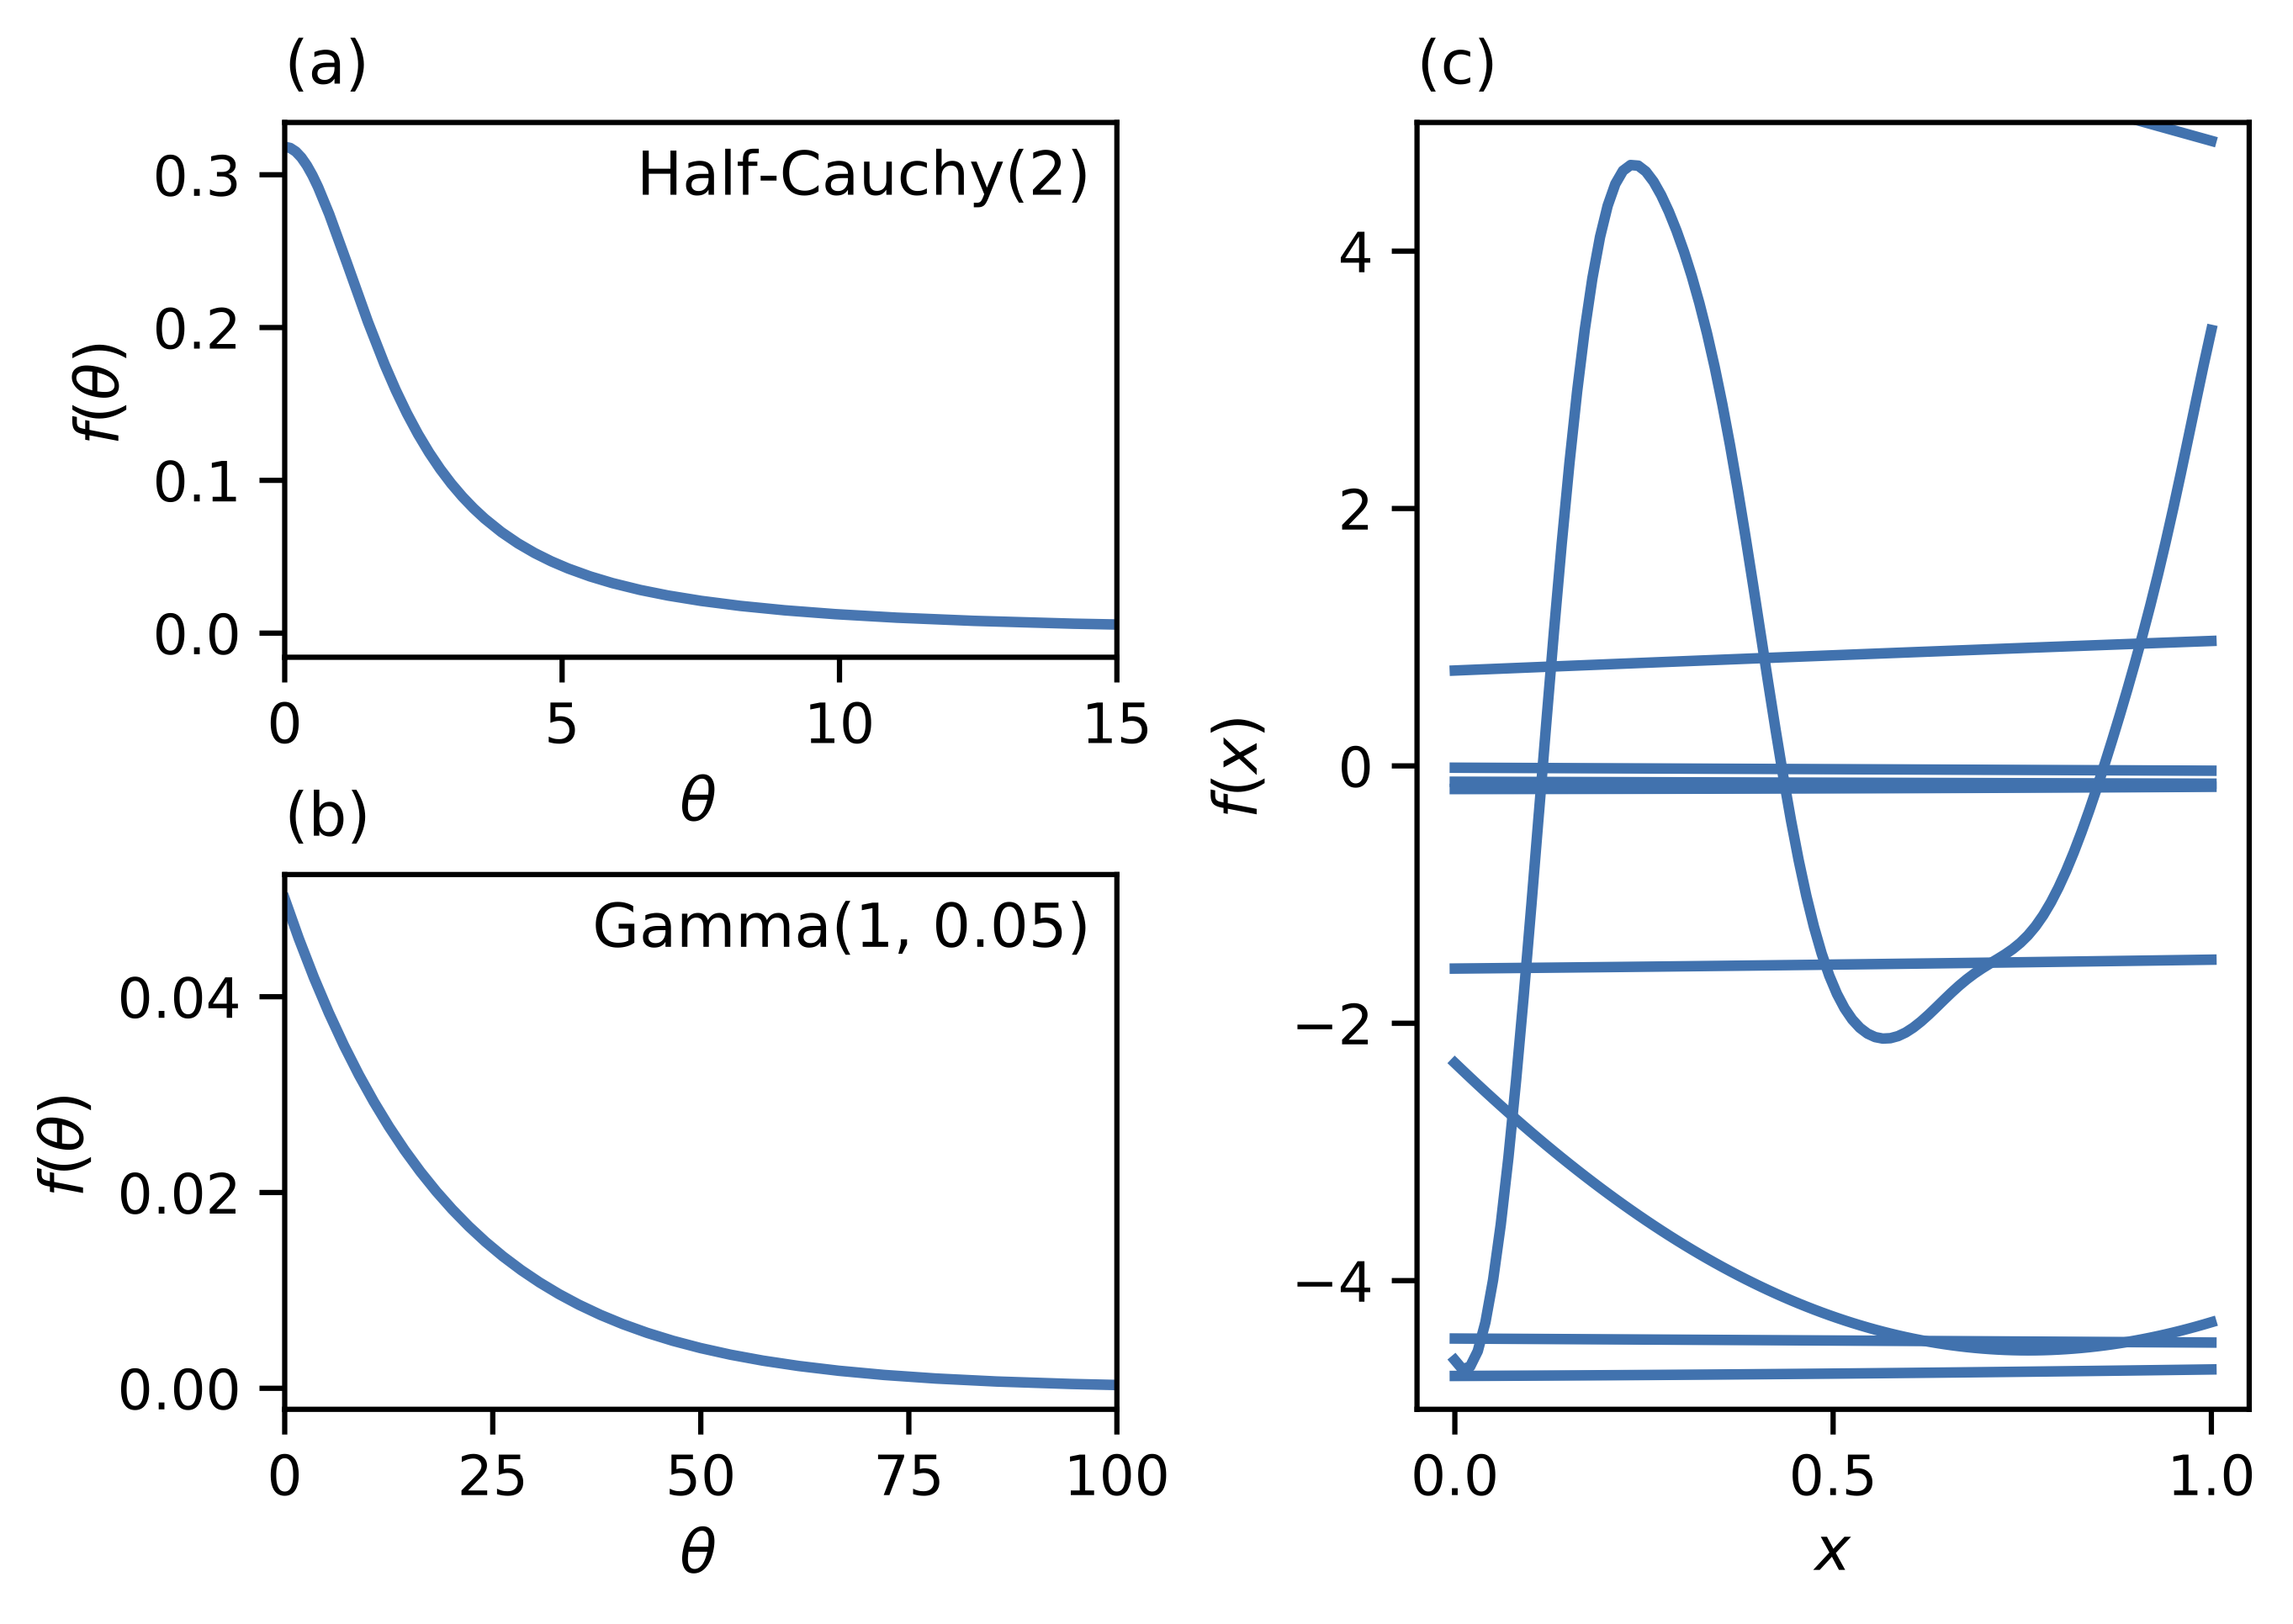
\includegraphics[width=0.8\textwidth]{chapters/msm_optimization/figures/prior_functions.png}
    \label{fig:priors}
\end{figure}

When modelling the response surface for visualisation and Bayesian optimisation, Maximum a posteriori (MAP) estimates  of the kernel hyper-parameters, $\theta = (\eta, \sigma_{n}, l_{1}, l_{2}, ...)$, with weakly informative priors were used. The prior distributions for the variance terms, $\eta$ and $\sigma_{n}$, were $\mathrm{half-Cauchy}(\beta=2)$ and the priors for the length-scale parameters, $l_{i}$, were $\mathrm{Gamma}(\alpha=1, \beta=0.05)$, these distributions are shown in Figure \ref{fig:priors} panels (a) and (b) respectively.  Examples of a 1D Gaussian process with a Gaussian covariance kernel with $\eta$ and $l$ drawn from these priors are shown Figure \ref{fig:priors} panel (c).  

The r\^ole of weakly informative priors is to exclude unrealistic or disallowed values of the parameters without imposing strong prior beliefs on the outcome. The half-Cauchy distribution  was used for $\eta$ and $\sigma_n$  based on its recommended use in other settings (\cite{polsonHalfCauchyPriorGlobal2012}). It was  only necessary for the scale of this distribution to give significant density in the range $0-5$ as the $\operatorname{VAMP-2}(k)$ score will lie in the range $[1,5]$ for alanine dipeptide and $[1, 4]$ for AADH which limits the possible values of $\eta$ and $\sigma_{n}$. The prior for $l$ was justified on the basis that, after scaling the predictors to lie in $[0, 1]$, values of $l \gg 1$ imply a flat response, meaning significant density for $l \gg 1$ isn't necessary. 

All predictors were scaled to lie in the range $[0, 1]$ to aid interpretation of the kernel length-scale parameters, $l$. Before scaling the integer predictors ($\tau$, $m$ and $n$) two input warpings, $T(\cdot)$, were considered: the identity $I(\cdot)$, and a logarithmic transformation, $\log(\cdot)$.  Input warpings are used \cite{snoekInputWarpingBayesian2014a} to mitigate the problems of modelling non-stationary functions using stationary GP models [TM: explain]. The categorical predictor, $\chi$, was dummy coded \cite{dalyDummyCodingVs2016} to give a $d$ dimensional vector of $1$s and $0$s. For example, the input vector, $\mathbf{x}$, for the first feature would be $\mathbf{x} = (1, 0, 0, 0, 0)$, for the second feature would be $\mathbf{x} = (0, 1, 0, 0, 0)$ and so on [TM: not clear]. 

In order to find the best GPR model for a given response surface, every combination of kernel function and  predictor warping was estimated using the MAP estimates for the kernel hyper-parameters and evaluated using the MSLL and SMSE metrics. This meant that for the response surface of alanine dipeptide eight different models were estimated (four different kernels and two warpings for $n$). For the response surface of AADH, with three integer predictors, $32$ different models were estimated (four different kernels and $2\times2\times2=8$ different predictor warpings). For each model both metrics were calculated used 10-fold cross validation and any model with $MSLL > 0$ or $SMSE > 1$ was discarded. The remaining models were ranked separately according to MSLL and SMSE ($R_{MSLL}$, $R_{SMSE}$) and the ranks combined according to $\sqrt{R_{MSLL}^2 + R_{SMSE}^2}$. This ranking method was used to ensure a balance between the two selection metrics compared to, say, the mean of the two ranks.  

All GPR modelling was performed with the Python package PyMC3 \cite{salvatierProbabilisticProgrammingPython2016} with some visualisation performed using package GPy \cite{gpy2014}. 

\subsection{Hyper-parameter relevance}\label{subsec:meth_rel}
The characteristic length-scales in equation \ref{eqn:kernel_form}, $l$, each correspond to a different predictor, or level of categorical predictor. They determine the covariance of the response between points with different values of that predictor. For example, with $l=1$ in an exponential kernel then inputs separated by $|x-x^{\prime}|= 1$ will on average have a covariance of $\exp^{-0.1}\simeq 0.9$. This means for large values of $l$ the response with respect to changes in $x$ will be flat, or in other words, $x$ is irrelevant to determining the response. This prompts the definition of \emph{relevance}, $R = \sfrac{1}{l}$: when $R$ is large, the small changes in $x$ result in larger changes in the response, meaning it is relevant to determining the response. Hereafter the kernel functions (equations \ref{eqn:kern_exp} - \ref{eqn:kern_m52}) will be parameterized interchangeably with $R$ and $l$ as convenient.  

The relevance of the MSM hyper-parameters is important for understanding and visualising the response surface and so to calculate the uncertainty in $R$ a fully Bayesian approach was used. After model selection using the maximum marginal likelihood models described in section \ref{subsec:rsm}, the GP model hyper-parameters were re-estimated by sampling the posterior distribution using Markov Chain Monte Carlo. A No U-Turn sampling algorithm, using two independent chains with $500$ tuning steps and $1000$ sampling steps. Convergence was checked using the R-hat statistic \cite{gelmanBayesianDataAnalysis2014}. 


\subsection{Bayesian Optimization}\label{subsec:bayes_opt}
Bayesian optimization is a method for optimizing ``black-box'' objective functions - those which can be sampled but are otherwise unknown \cite{shahriariTakingHumanOut2016}. The response of an MSM to its hyper-parameters is a black-box objective function because it is not possible to determine the response without first fitting the MSM. Bayesian optimisation is a type of sequential model based \cite{hutterSequentialModelbasedOptimization2011} optimisation technique. These techniques entail first sampling the response of the objective function over a search space to create a trial data set. A statistical model called the \emph{surrogate function}, which serves as a proxy for the objective function, is built using the sampled responses. An utility function, known as the \emph{acquisition function}, determines the anticipated utility of a set of inputs in optimizing the objective function, based on the predictions and uncertainty in the surrogate function.  The objective function is then sampled using the set of inputs which maximize the acquisition function. This new trial is added to trial data set and process repeated. This algorithm (with modifications discussed below) is summarised in algorithm \ref{alg:bayes_opt}. 

\begin{algorithm}\label{alg:bayes_opt}
\KwData{Trial data: $\mathcal{D}_{N} = \{(y_{1}, \mathbf{x}_{1}), ...,(y_{N}, \mathbf{x}_{N}) \}$}
\KwData{Search space grid: $\mathbf{X} = \{(\chi_1, \tau_1, m_1, n_1), ...,(\chi_{M}, \tau_{M}, m_{M}, n_{M})\}$}
\KwResult{$\mathbf{x}^{*} = \argmax_{\mathbf{x}}{f(\mathbf{x}; \mathcal{D}_{N+p})}$}
\BlankLine
\For{$i\leftarrow N$ \KwTo $N+p$}{
    estimate GP surrogate $f(\mathbf{x}; \mathcal{D}_{i})$\;
    calculate incumbent: $\mu^{*} = \argmax{f(\mathbf{x};\mathcal{D}_{i})}\ \mathrm{s.t.}\ (y, \mathbf{x}) \in \mathcal{D}_{i}$\;
    estimate acquisition function: $\alpha_{\mathrm{EI}}(\mathbf{x}; \mathcal{D}_{i})\ \mathbf{x} \in \mathbf{X}$\;
    select candidate: $\mathbf{x}_{i+1} = \argmax_{\mathbf{x}}\alpha_{\mathrm{EI}}(\mathbf{x}; \mathcal{D}_{i})\ \mathrm{s.t.}\ (\mathbf{x} \in \mathbf{X})\ \&\ (\mathbf{x} \notin \mathcal{D}_{i})$\;
    query objective function to obtain: $y_{i+1}$\;
    augment data: $\mathcal{D}_{i+1} \leftarrow \{\mathcal{D}_{i}, (y_{i+1}, \mathbf{x}_{i+1})\}$
}
\caption{Bayesian Optimisation.}
\end{algorithm}

In principle, any function capable of predicting a response along with its uncertainty can be used in Bayesian optimisation, examples include random forests [] and Tree Parzen estimator models []. However Gaussian process models are commonly used [][][], especially for hyper-parameter optimisation problems\cite{bergstraAlgorithmsHyperParameterOptimizationa}\cite{martinez-cantinBayesOptBayesianOptimization2014}, due to their flexibility in modelling non-linearities; their natural incorporation of uncertainty due to data sparsity; the resulting analytical expressions for acquisition functions, and the fact that they are closed under sampling \cite{NIPS2012_4522}\cite{brochuTutorialBayesianOptimization2010} (this last fact essentially asserts that updating a GP with additional observations the model remains a GP). 

There are a wide variety of candidate selection policies, corresponding to different acquisition functions, each of which trades off exploration or the search space with exploitation of more certain optima of the response function. Improvement based policies, such as probability of improvement \cite{Kushner1963} and expected improvement \cite{mockus1978application}, suggest candidates that lead to increases over an incumbent target, $\mu^{*}$.  Optimistic policies, such as the upper confidence bound \cite{icml2010_129}, minimize the cumulative regret (the sum of the difference between the true maximum and the function evaluations at the candidate inputs). Other policies are based on information theoretic approaches (such as the.....) 

This work uses the the expected improvement, $\mathbb{E}[I]$ where the improvement, $I$, is defined :  
\begin{equation}
    I(\mathbf{x}, f, \mu^{*}):=(f(\mathbf{x}) - \mu^{*}) \mathbb{I}(f(\mathbf{x}) > \mu^{*})
\end{equation}

Here the $\mathbb{I}$ is an indicator function which prevents the improvement from being negative and the incumbent is defined as the maximum of the response surface \emph{at the trial values}. The expected improvement is the expectation of $I$, averaged over the distribution of $f(\mathbf{x})$ which can be calculated analytically for maximum marginal likelihood GPs as: 

\begin{align}
        \alpha_{EI}(\mathbf{x}) := &  \mathbb{E}\left[I(\mathbf{x}, f(\mathbf{x}), \mu^{*})\right] \\
         =  &(\mu(\mathbf{x}) - \mu^{*})\Phi\left( \frac{ \mu(\mathbf{x}) - \mu^{*} }{\sigma(\mathbf{x})} \right ) + \sigma(\mathbf{x})\phi\left( \frac{ \mu(\mathbf{x}) - \mu^{*} }{\sigma(\mathbf{x} } \right )
\end{align}

Here $\Phi, \phi$ are the normal cumulative and probability distribution functions respectively, and $\sigma(\mathbf{x})$ is the variance of the GP at the point $\mathbf{x}$. It is possible to take the expectation over both the distribution of $f$ and of the GP hyper-parameters $\theta$ and this has been suggested and shown to be effective \cite{NIPS2012_4522}). However this was not done in this work because the extra computational cost involved. The candidate MSM hyper-parameters were determined as those which had the highest expected improvement as calculated on a $4 \times 100 \times 20 \times 100$ ($\chi \times \tau \times m \times n$) evenly spaced grid over the search space.

It was observed during these experiments that the same candidate hyper-parameters were being proposed by the algorithm. This was deemed due to the granularity of the grid used in the maximisation of the acquisition function. To ensure that each candidate hyper-parameter is unique, the Bayesian optimisation algorithm was modified so that only  hyper-parameters sets not already in the trial data set were considered as candidates. This is reflected in the conditions on the `select candidate' step of algorithm \ref{alg:bayes_opt}.

Although not explicitly discussed in the theoretical literature, software packages seed the process with randomly selected hyper-parameter trials so that the initial response surface contains some information, rather than just a random draw from the prior function distribution. The default number of trials in Bayesian optimisation software packages lie in the range x - y. Conventional advice \cite{harrelRegressionModelingStrategies2015} for parametric models (e.g. multi-variable linear regression) puts the required number of observations for estimating parameters as at least $15$ observations per parameter. An appropriate number was partially explored in this work. 

\subsection{MSM Optimisation}
Bayesian optimisation was used to determine whether the maximum of the response surface estimated from the trial data set could be improved and whether this maximum could be reached with smaller trial data set.

An exploratory optimisation procedure was first performed on the alanine dipeptide system to demonstrate its effectiveness and to determine how many randomly sampled seed trials are needed to initalise the BO procedure, $N_{seed}$. $p=10$ steps of the BO algorithm was performed on five random subsets of the alanine dipeptide trial data set with $N_{seed}=30, 50$ trials (stratified over the features $\chi$), corresponding to $15, 25$ trials per predictor. As discussed further in section \ref{subsec:ala1}, $25$ trials per predictor was found to result in satisfactory improvement in the incumbent.  

For AADH two optimisation experiments were performed:
\begin{enumerate}
    \item $p=50$ steps of Bayesian optimisation was performed using a response surface seeded with all of the randomly sampled hyper-parameter trial data ($N_{seed}=361$);
    \item $p=50$ steps of Bayesian optimisation was performed on five subsets  of the hyper-parameter trial data with  $N_{seed}=100$, which corresponded to $25$ trials per predictor.
\end{enumerate} 

In both cases the combination of input warping and kernel-type  were determined by selecting the highest ranked model using the MSLL and SMSE metrics (equations \ref{eqn:msll} and \ref{eqn:smse}). The of the kernel hyper-parameters were determined by maximizing the marginal log-likelihood, equation \ref{eqn:marg_llike}. 

\section{Results and discussion}
\subsection{Alanine Dipeptide}\label{subsec:ala1}
\subsubsection{Response surface}\label{subsubsec:ala_rsm}

\begin{figure}[p]
    \centering
    \mycaption{The $\operatorname{VAMP-2}$ scores of the hyperparameter trials for MSMs of alanine dipeptide. The test response, $f^{test} = f(\chi, n; \mathbf{X}^{test})$ is shown in blue, panels: a, c, e, g, i,  while the degree of over-fitting, $f^{train} - f^{test}$, is shown in orange, panels: b, d, f, h, j. Each row represents a different value of the feature ($\chi$) and the horizontal axis represent the number of clusters, ($n$). Each trial was scored with $20$ iterations of 50:50 shuffle split cross validation. The error bars represent the $25$th and $75$th quantiles of the cross-validation folds. 
    The features are ordered according to the mean of the their test scores.}
    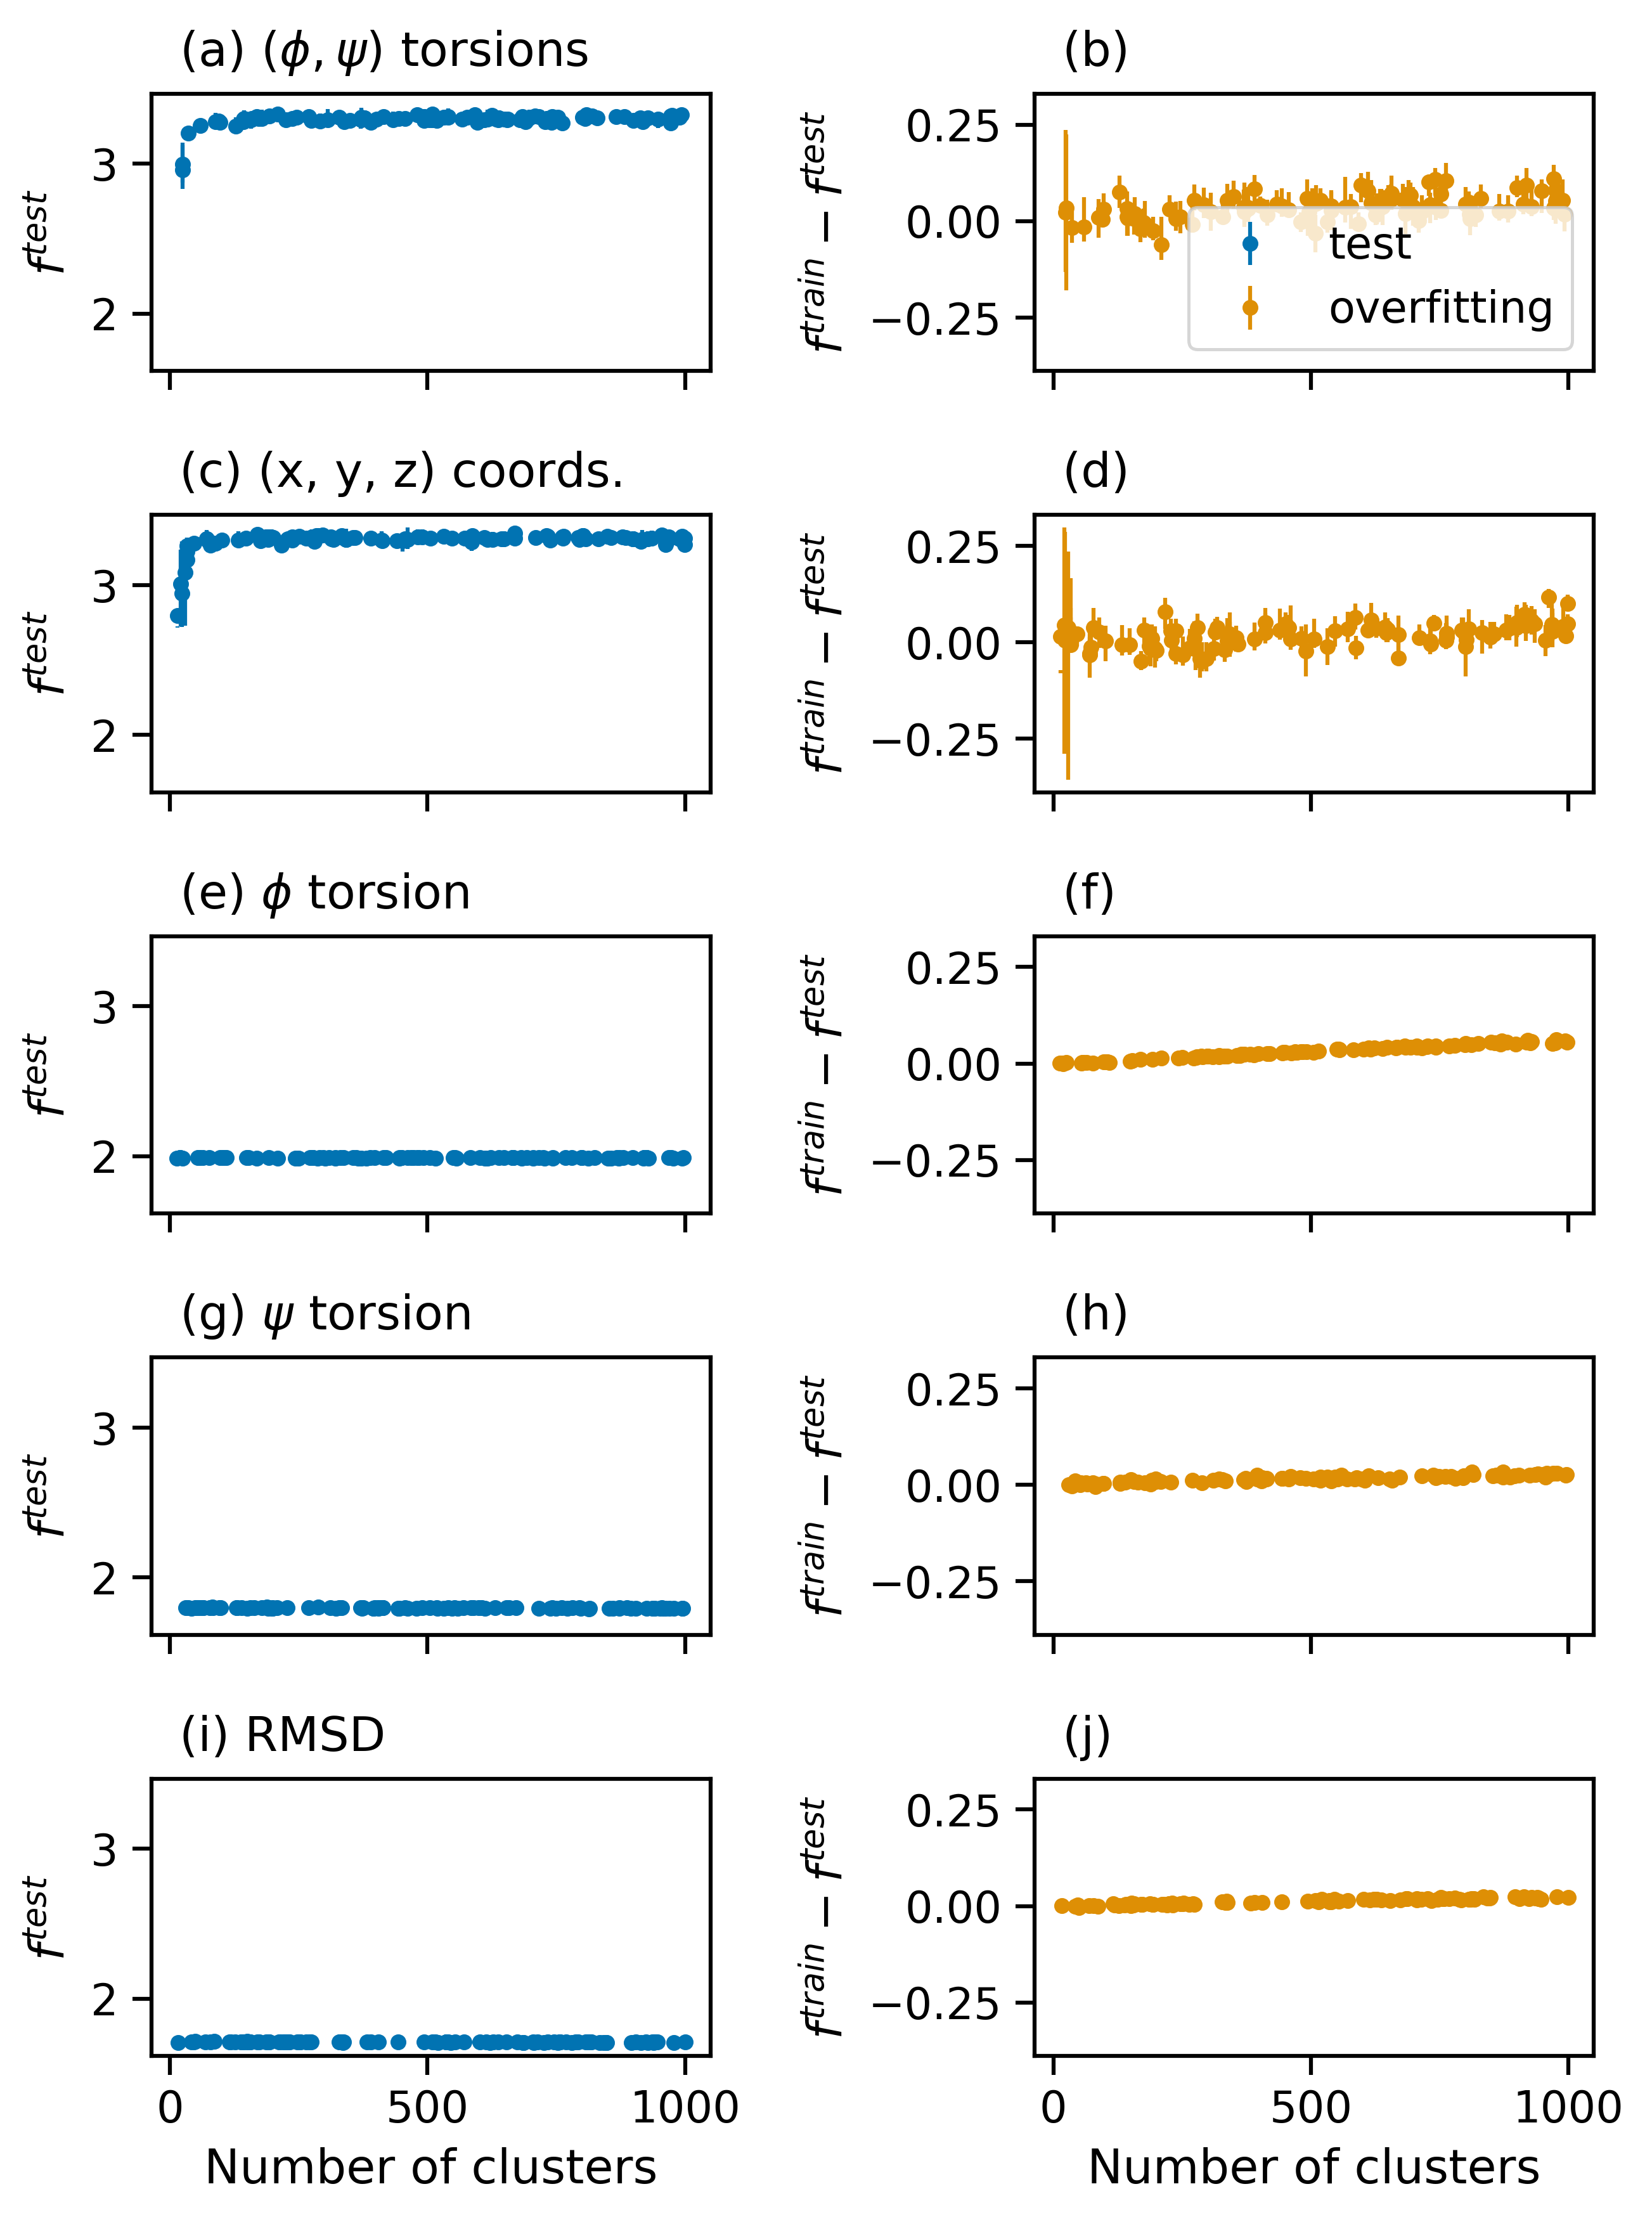
\includegraphics[height=0.8\textheight]{chapters/msm_optimization/figures/ala1_train_test_results.png}
    \label{fig:ala1_train_test}
\end{figure}

The average MSM response for each trial are shown in figure \ref{fig:ala1_train_test}. The test response ($f^{test} = f(\chi, n; X^{test})$, blue points) and the difference between train and test response, ($\Delta f = f^{train} - f^{test}$, orange) are shown as a functions of $n$. The features are ordered according to the  mean of the test response. As expected [][] the  $(\phi, \psi)$ feature has the highest average response, but unexpectedly, the heavy atom $(x,y,z)$ coordinates feature performs just as well. 

The difference between the train and test response, the \emph{over-fitting} reflects the consistency between the eigenvectors estimated on the training data and those implied from the time-lagged covariance and overlap matrices ($C$ and $\Pi$  in \ref{eqn:tran_def}) estimated  on the test data. So a small $\Delta f$ implies that the picture of the relaxation processes are represented equally well, with the given hyper-parameters, in the training and test data (even if they're both inaccurate pictures). This will arise, as is likely in this case, with large volumes of data.    

The response surface (figure \ref{fig:ala1_response}) was modelled as a Gaussian process with $\chi$ and $n$ as predictors. A Mat\'{e}rn 5-2 kernel and logarithmic input warping of $n$ were chosen using a combination of the MSLL and SMSE model selection criteria (see table \ref{tab:ala2_fit_results} for the full model selection results). The choice of logarithmic warping of $n$ is unsurprising given that the response for the $(\phi, \psi)$ and $(x,y,z)$ features (panels (a) and (c) in figure \ref{fig:ala1_train_test}) is a clearly non-stationary process: the covariance of the response with respect to changes in $n$ is much lower for $n\leq 100$ than for $n\geq 100$ where the response reaches a plateau. The log transformation smooths the response with respect to $n$ and makes the assumption of a stationarity more plausible.  This response surface fits the observed data well, both in terms of the mean response and its uncertainty. There are a number of features of the response surface which are worth discussing. 

\begin{figure}
    \centering
    \mycaption{The response surface of alanine dipeptide as a function of the feature, $\chi$ (panels a - e) and number of clusters, $n$ (horizontal axis). The features are ordered according to their average response. A Mat\'{e}rn 5-2 kernel and logarithmic warping of the predictor $n$  was used. The blue line is the mean of the surface, the blue shaded bands represent the uncertainty ($\pm2\sigma$ excluding the noise term $\sigma_{n}$, and the black crosses are the observed values (the cross validated mean of VAMP-2). Note the differing vertical axis scales. This was to allow the curvature of the response surface to be visible.}
    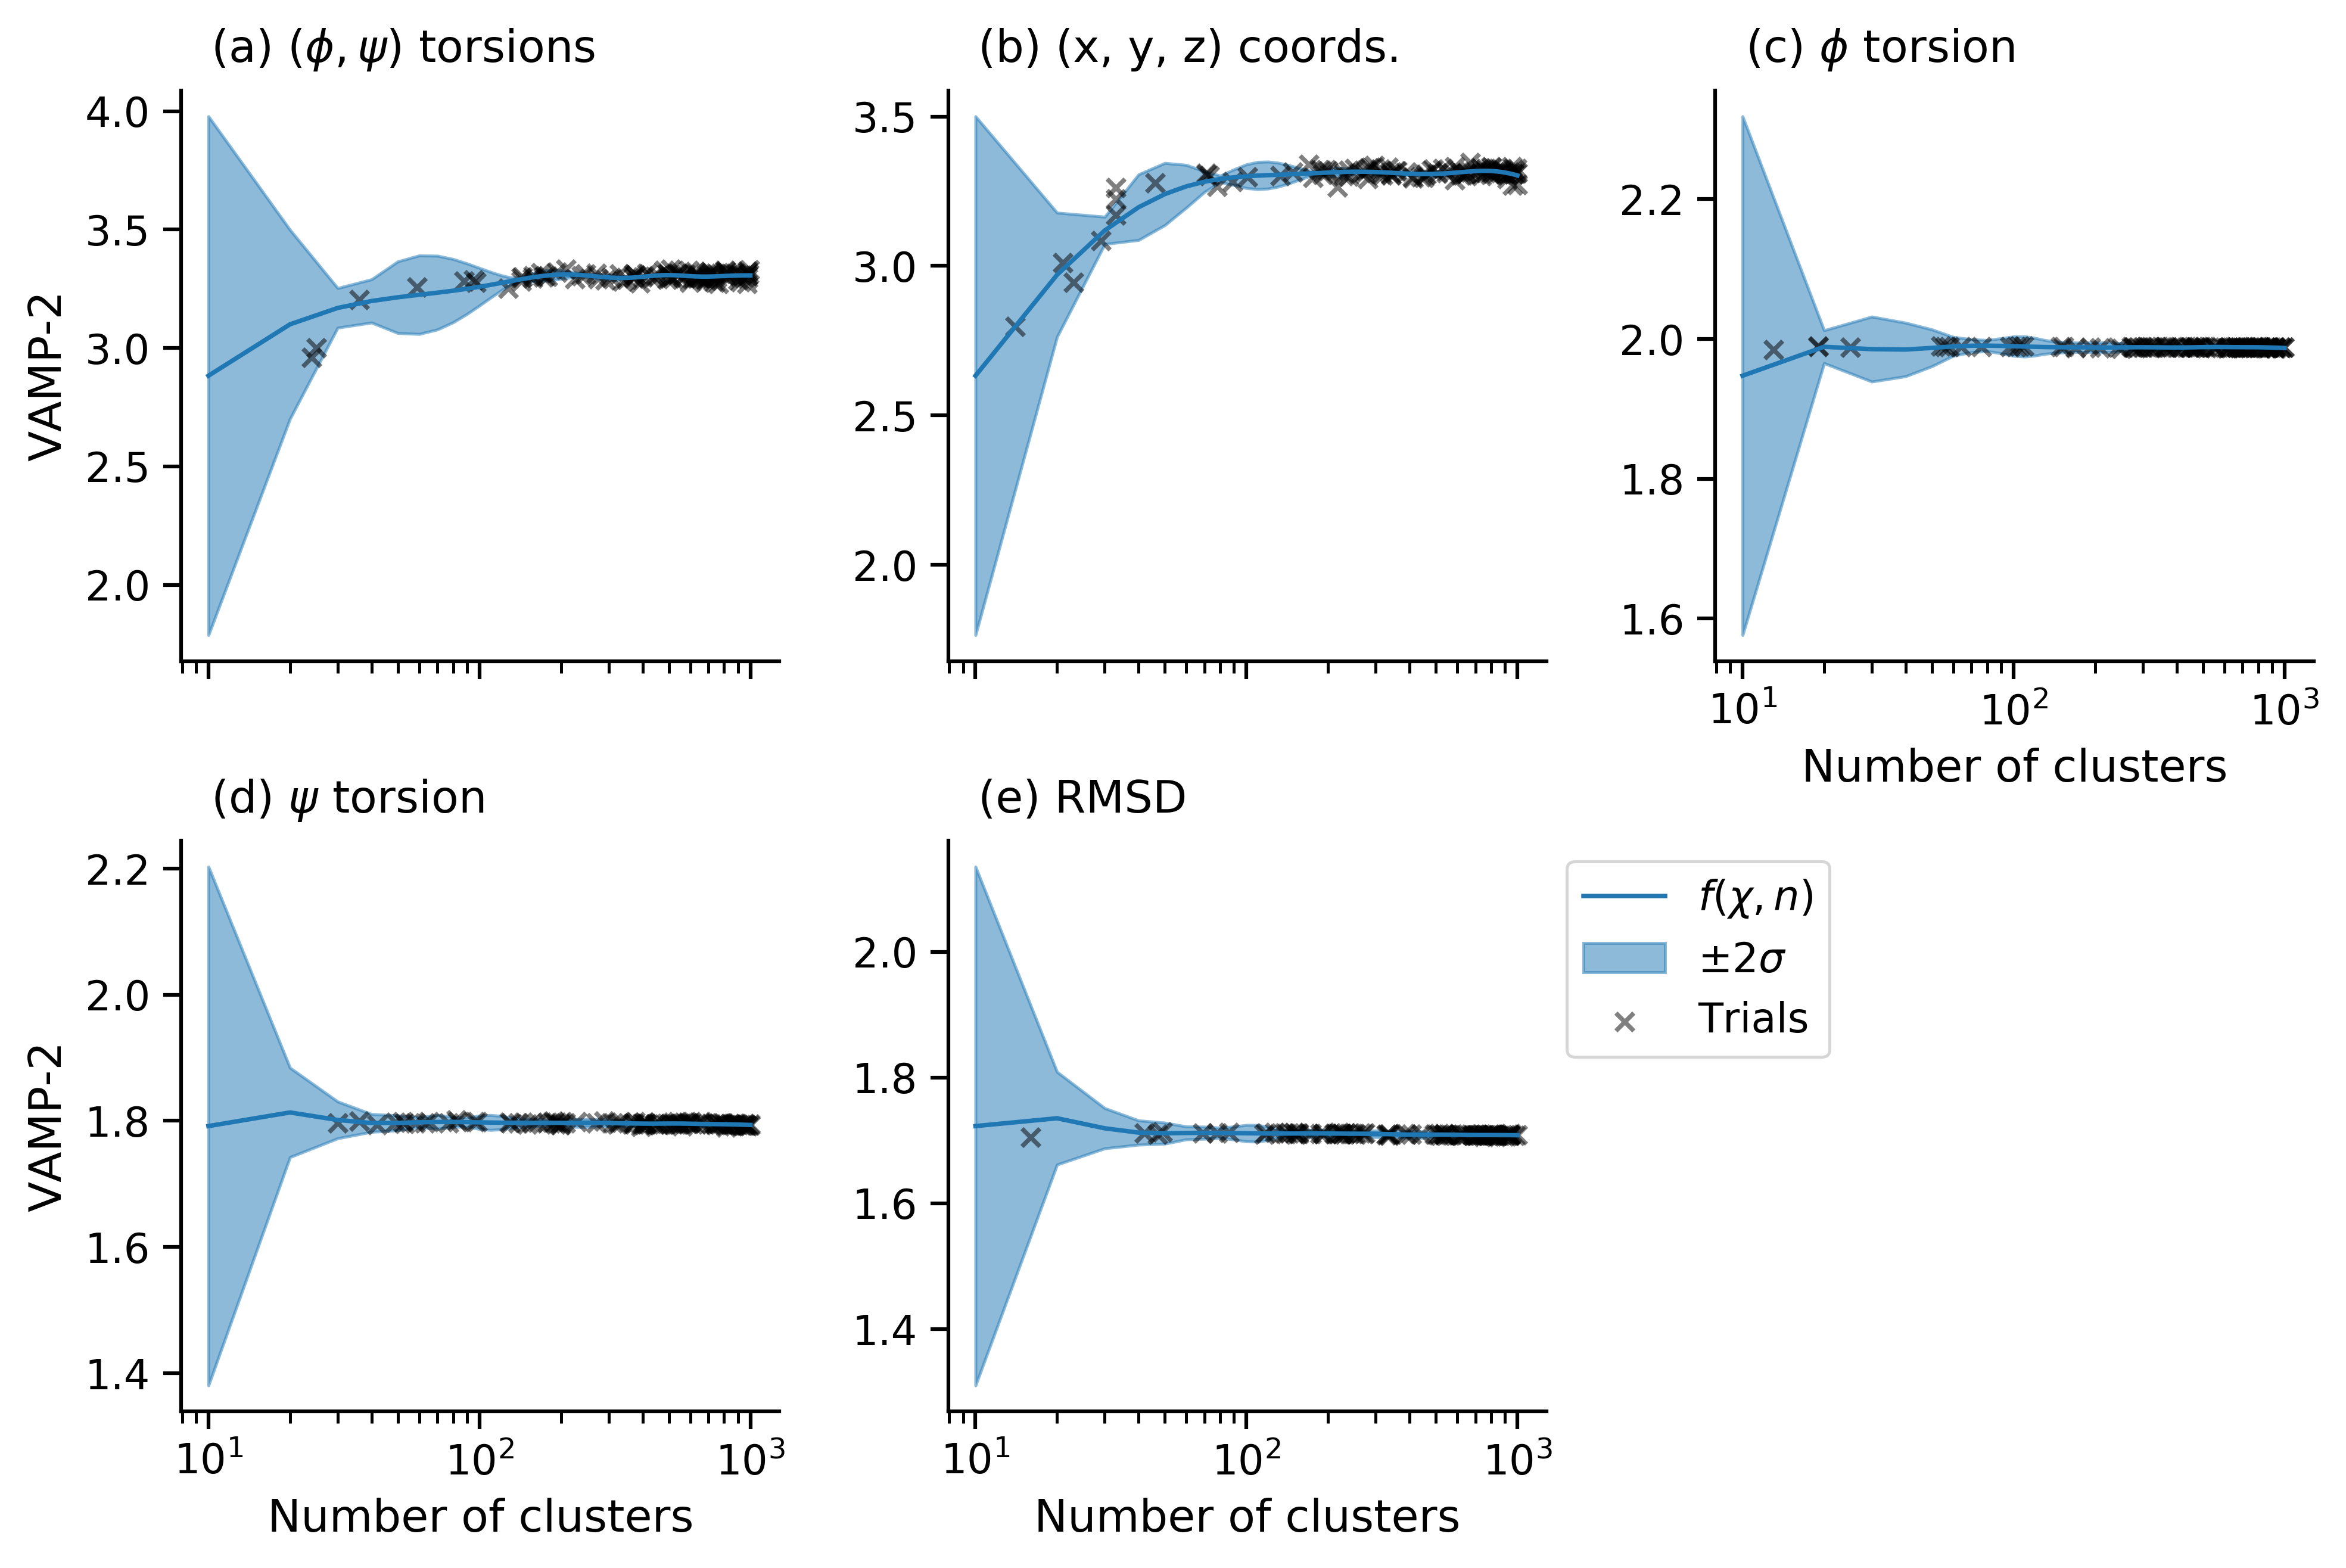
\includegraphics[width=0.8\textwidth]{chapters/msm_optimization/figures/ala1_response_surface.png}
    \label{fig:ala1_response}
\end{figure}

First, there is a decrease in response as $n \rightarrow 10$ for the $(\phi, \psi)$ and $(x,y,z)$ coordinate features but not the remaining features (although this is due to the sparse sampling for $n<20$ and no sampling for $n<10$). This is expected from previous studies \cite{wuVariationalApproachLearning2019}\cite{mcgibbonVariationalCrossvalidationSlow2015} and is due to decreasing eigenfunction discretization error, $\delta$  \cite{prinzMarkovModelsMolecular2011} as a $n$ increases. In the language of statistical learning theory \cite{friedman2001elements}, this is the high ``Bias'' regime of the ``Bias-variance'' trade-off. The discretizaton error for the $i$'th normalized eigenfunction of an MSM $\Psi_{i}$ is given by [TM: needs more explanation]: 

\begin{equation}
    \delta_{i} \equiv\left\|\Psi_{i}\left(\mathbf{z})-\hat{\Psi}_{i}(\mathbf{z}\right)\right\|_{\pi, 2}=\left(\int_{\Omega} d \mathbf{z} \pi(\mathbf{z})(\Psi_{i}(\mathbf{z})-\hat{\Psi}_{i}(\mathbf{z}))^{2}\right)^{1 / 2}
\end{equation}
\begin{figure}
    \centering
    \mycaption{The discretization error of the dominant right eigenfunction of alanine dipeptide as a function of the number of cluster centers. The feature used is the $\phi$ backbone torsion. Panel (a) shows the free energy along this feature. Panels (b), (c) and (d) show the normalized MSM right eigenfunction (blue line) estimated $n=2, 10$ and $50$ cluster centers respectively. This is compared with the same eigenfunction estimated with $n=500$ cluster centers (black line). The red shaded area represents the difference between the two eigenfunctions. The discretization error, labelled $\delta$ is the integral of the red area. The $VAMP-2$ score is also labelled for comparison.}
    \label{fig:ala1_evcompare}
    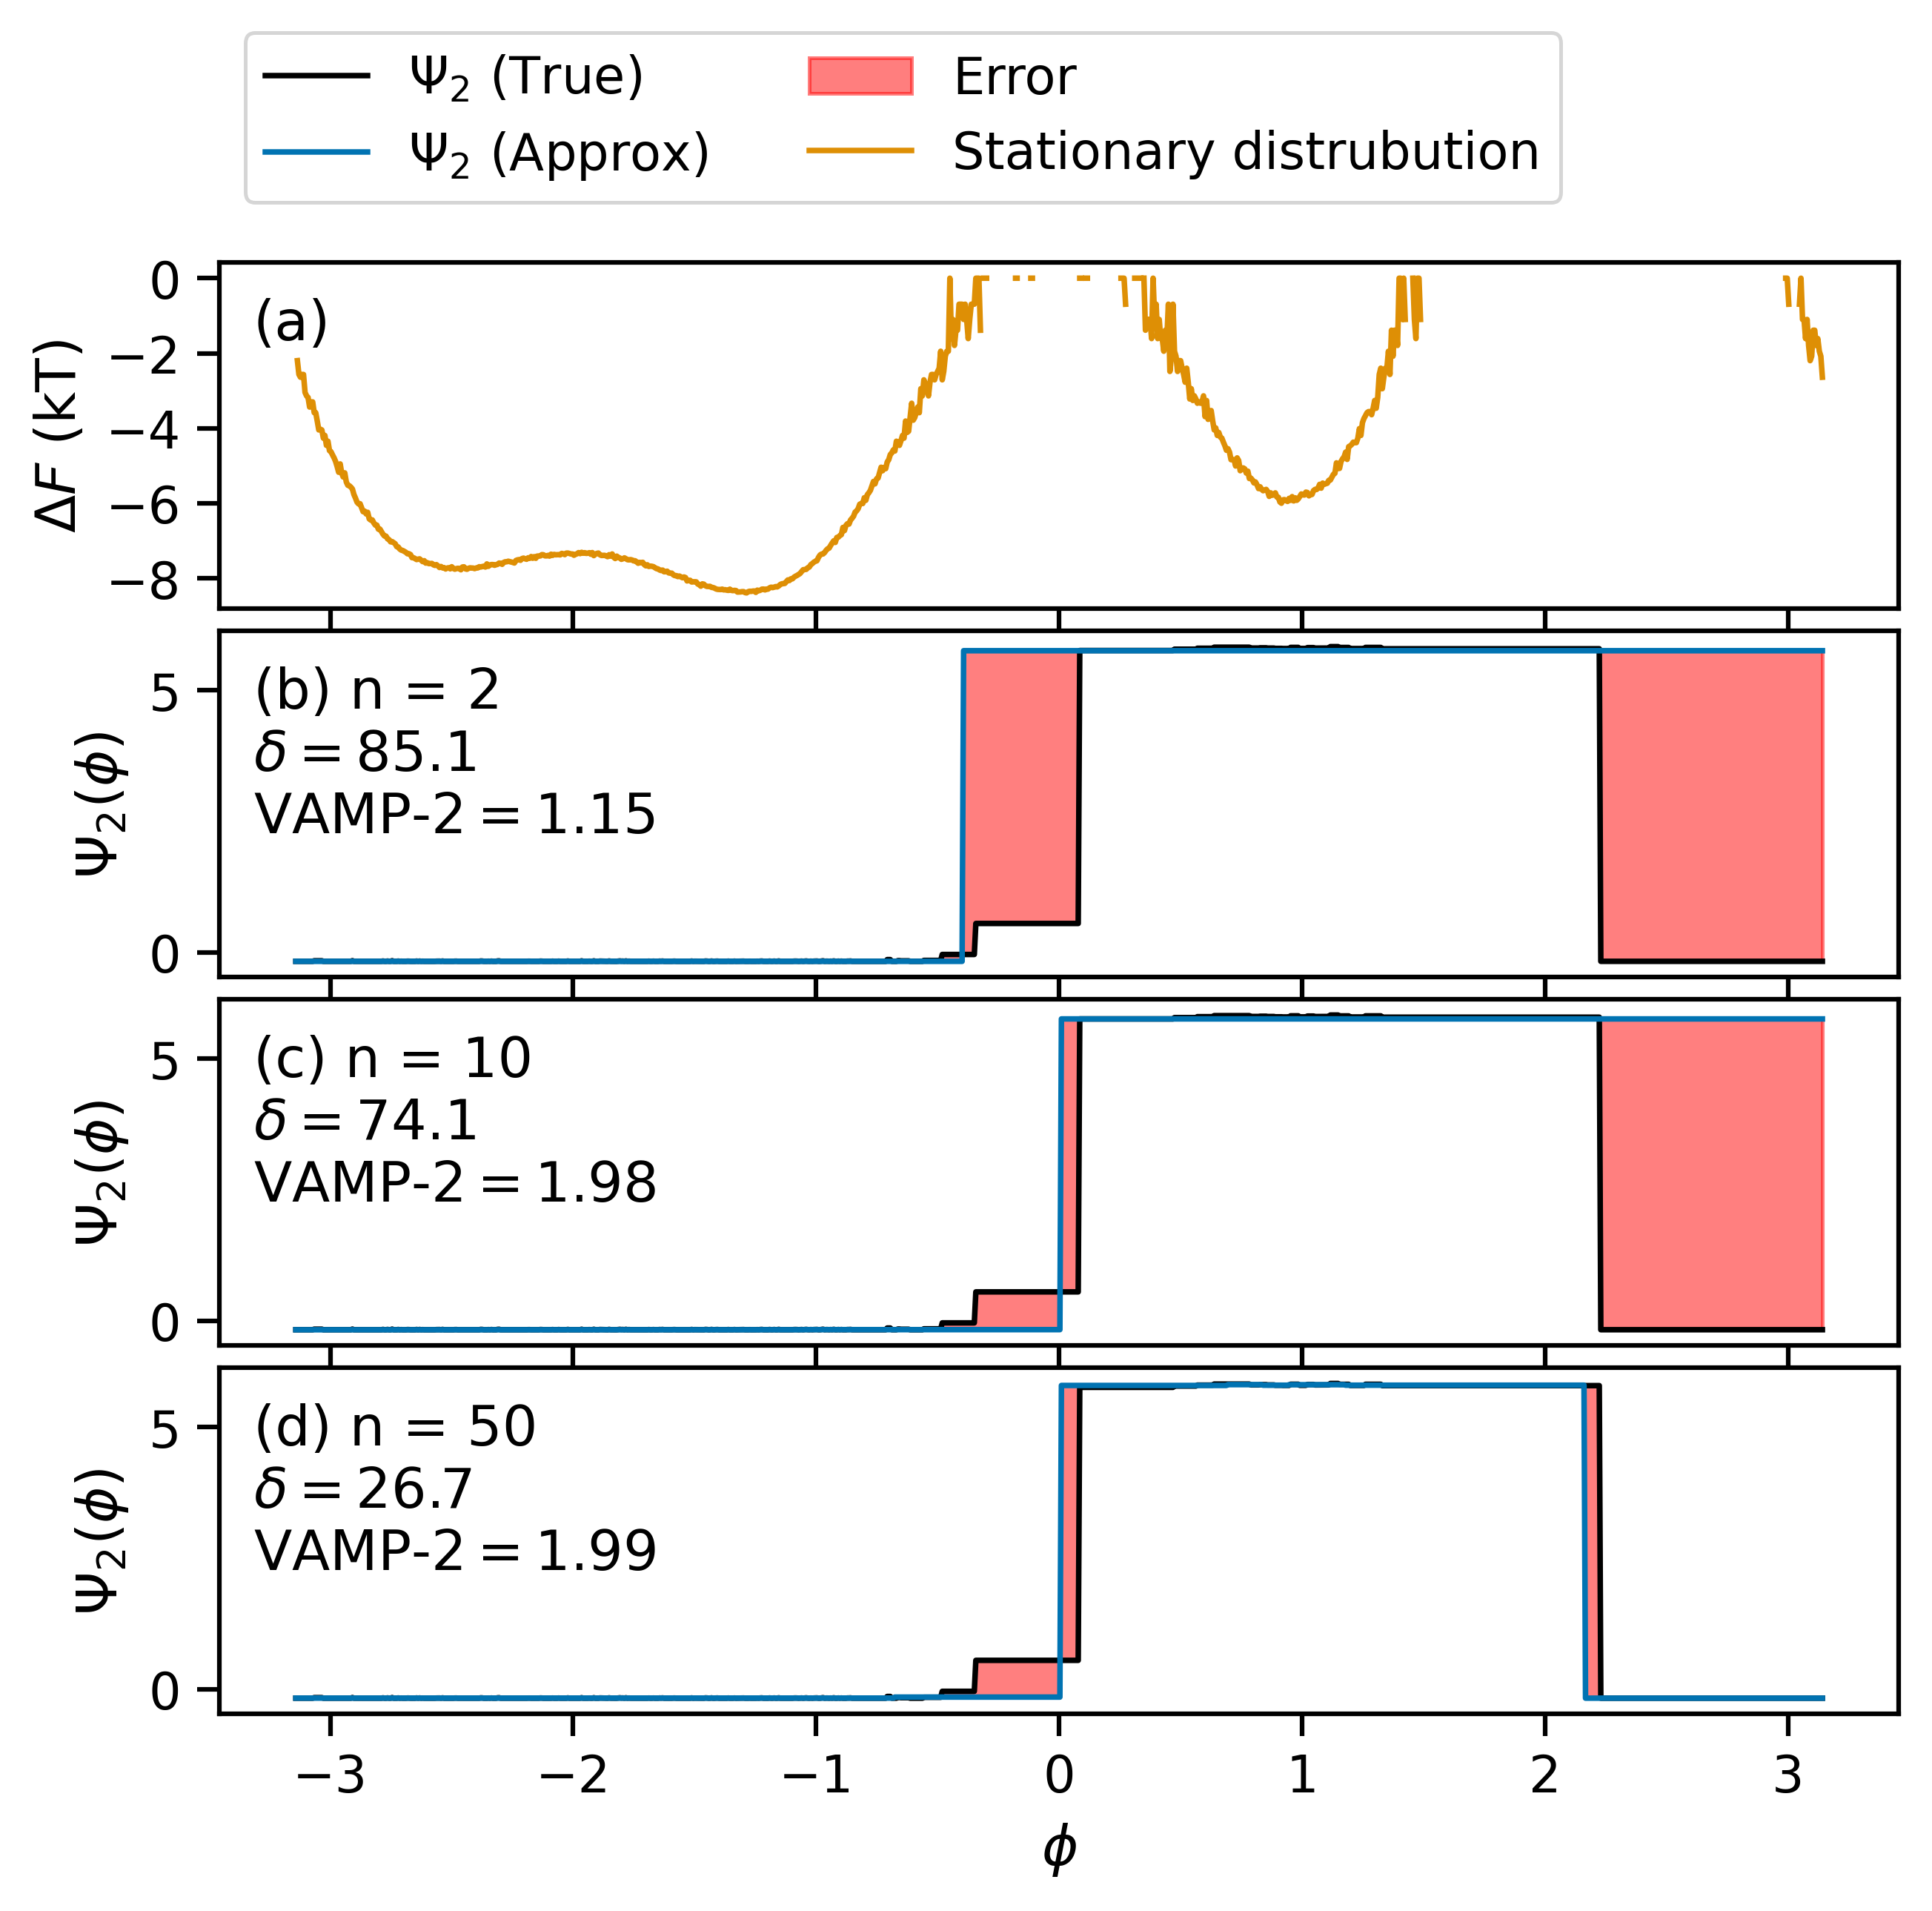
\includegraphics[width=0.8\textwidth]{chapters/msm_optimization/figures/ala1_ev_n_compare.png}
\end{figure}

Here $\mathbf{z}$ are the coordinates of state space (e.g. Cartesian coordinates), $\pi$ is the stationary distribution and the integral runs over all of the state space, $\Omega$. The integrand is the difference between the true normalized eigenfunction $\Psi$ and approximate eigenfunction $\hat{\Psi}$. 

To get a sense of how the response and the discrietisation error are related, approximations to dominant eigenfunction, $\hat{\Psi}_{2}$, for the $\phi$ feature, are plotted in figure \ref{fig:ala1_evcompare}. For reference, panel (a) shows the stationary distribution. The truncation around the values of $\phi \simeq 0, 2$ is due to the temporal resolution of the MD trajectories. The Panels (b), (c) and (d) show the difference between the true second normalised eigenvector ( black line labelled $\Psi_{2}$ (True)) and the same eigenvector estimated with $2, 5, 50$ basis states (blue line, labelled $\Psi_{2}$ (Approx.)). The true eigenvector was taken as $\Psi_{2}$ estimated with $n=500$ basis states (i.e. with negligible discretization error) rather than the eigenvector measured in the $(\psi, \phi)$ space for simplicity. The red shaded area shows the discretization error which is summed to give $\delta$. As $n$ increases from $2$ to $10$ to $50$, $\delta$ decreases (from $67.98$ to $51.54$ to $1.99$) while the response increases from $1.25$ to $1.98$ to $1.99$. For this feature, and likely for the other one-dimensional features ($\psi$, RMSD) the largest decrease in VAMP-2 occurs below $n=10$ which explains why the drop in response with decreasing $n$ is not observed. 

Second, the response for all features for $n > 100$ is constant. This is a result of the volume of MD simulation data. The discretisation error will eventually become negligible for all of the  non-trivial eigenvectors used in the VAMP-2 score as $n$ increases. As already mentioned, this explains the rapid increase in the response for $n<100$. In general, as $n$ increases the statistical uncertainty in the elements of the estimated transition matrix will increase and the model enters the high variance regime of the ``Bias-variance'' trade-off.  However, with the large volume simulation data the number of observations ($750\times(1000-9) = \num{743250}$ pairs of observed transitions) is comparable to the degrees of freedom for a reversible MSM \cite{trendelkamp-schroerEstimationUncertaintyReversible2015b} ($\sfrac{1}{2}n(n-1)+n-1=\num{500499}$ for $n=1000$).   

Third, large uncertainty of response surface for $n \leq 20$ is a result of the logarithmic warping  of $n$ and the comparatively sparse sampling in this region (as all sampling was done without prior logarithmic warping). 

Fourth, it is clear from inspection of figure \ref{fig:ala1_response} that the most relevant hyperparameter for determining the test response is the feature, $\chi$, while the number of cluster centres,  $n$, is almost irrelevant. This information is encoded in the learned hyper-parameters of a Gaussian process which will be of benefit in more complicated systems with more than two hyperparameters. 
 
\subsubsection{Hyper-parameter relevance}\label{subsubsec:ala_relevance}

\begin{figure}
    \centering
    \mycaption{The relevance of the hyper-parameters of alanine dipeptide. The distribution of the parameters of the response surface (shown in figure \ref{fig:ala1_response}) were estimated using MCMC. The relevance of the features (levels of $\chi$) are shown in blue, labelled `Feature'. The relevance of the log-transformed number of cluster centres, $n$ is shown in orange (labelled `Other').}
    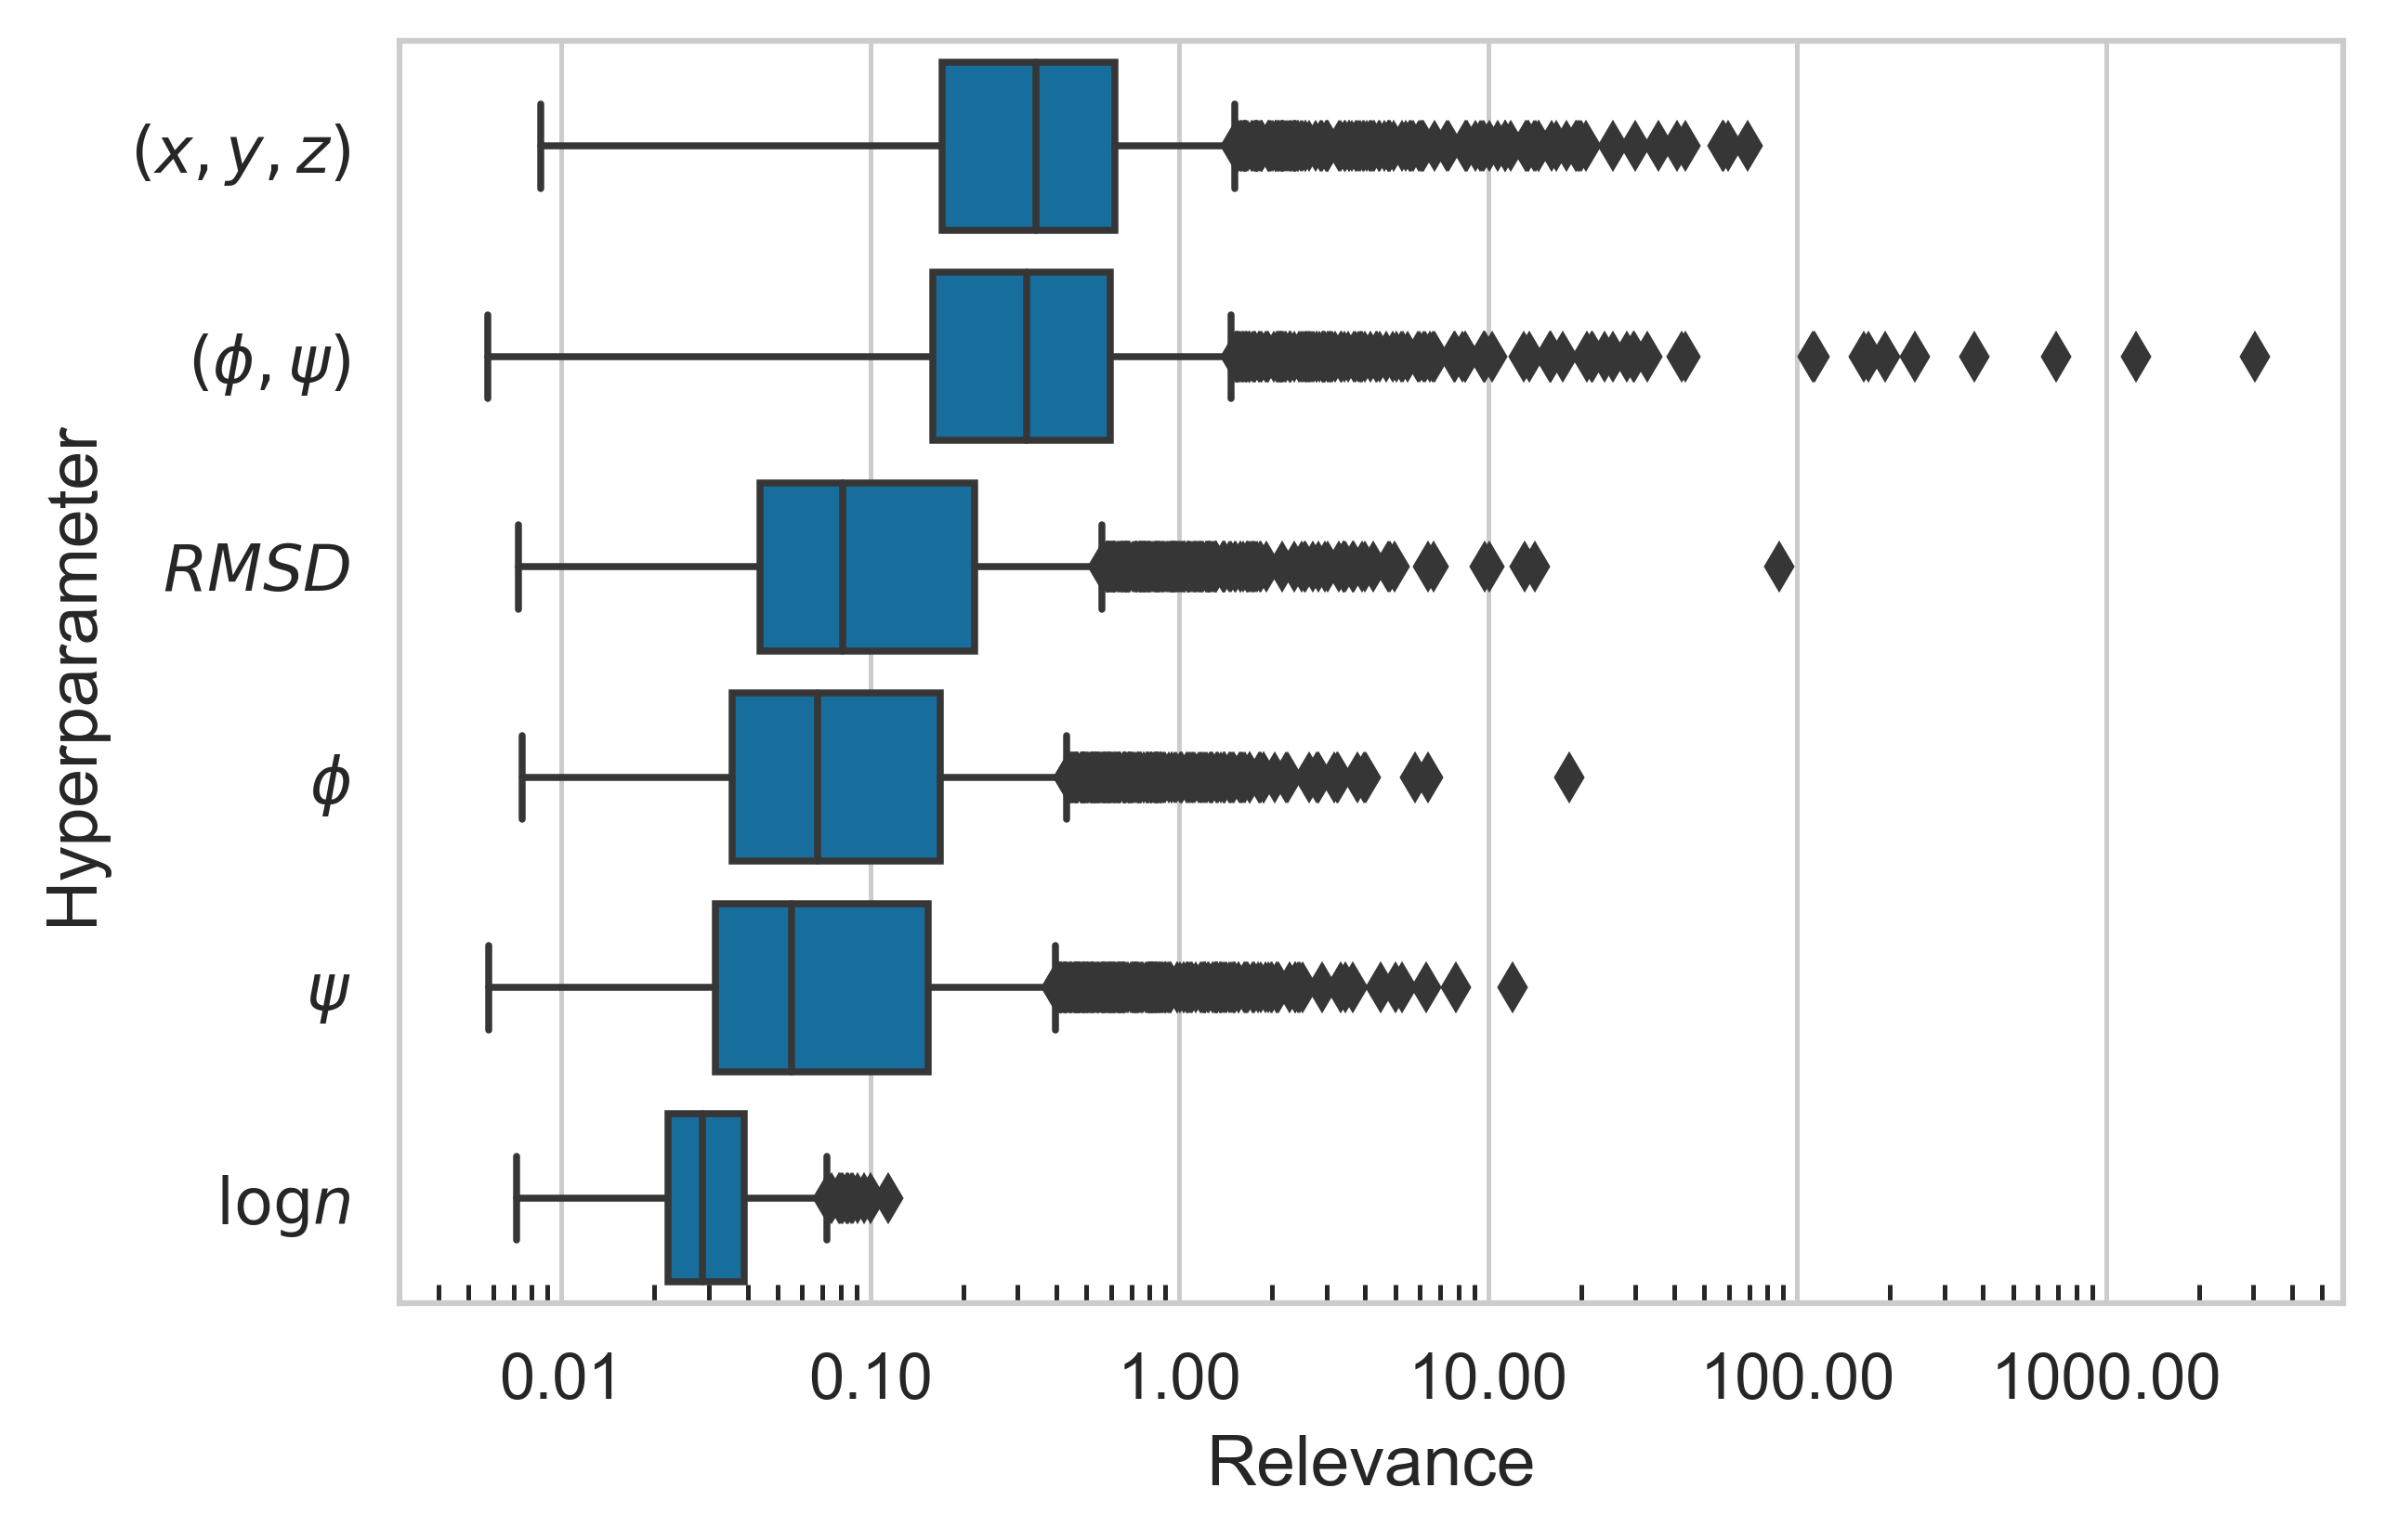
\includegraphics[width=0.8\textwidth]{chapters/msm_optimization/figures/ala1_relevance.png}
    \label{fig:ala1_relevance}
\end{figure}

\begin{table}
    \centering
    \mycaption{Median and $\SI{95}{\percent}$ credible intervals for the kernel hyper-parameters of the alanine dipeptide response surface estimated using MCMC. The length-scale parameters in \ref{eqn:kernel_form} are re-written here as relevances.}
    \begin{tabular}{|l|l|l|}
    \hline
                          Hyper-parameter &    Median & $\SI{95}{\percent}$ C.I. \\
    \hline\hline
     $R_{(\phi, \psi)\ \mathrm{torsion}}$ &  0.321 & 0.020-4.456 \\
        $R_{(x, y, z)\ \mathrm{coords.}}$ &  0.344 & 0.024-5.572 \\
             $R_{\phi\ \mathrm{torsion}}$ &  0.068 & 0.015-1.176 \\
             $R_{\psi\ \mathrm{torsion}}$ &  0.056 & 0.013-1.327 \\
                               $R_{RMSD}$ &  0.081 & 0.016-1.406 \\
                          $R_{\log{(n)}}$ &  0.029 & 0.013-0.063 \\
                                   $\eta$ &  2.518 & 1.141-5.530 \\
                               $\sigma_n$ &  0.006 & 0.006-0.007 \\
    \hline
    \end{tabular}
    \label{tab:ala1_rel_post}
\end{table}

This last observation can be quantified and understood by estimating the relevance of each predictor. The posterior distributions of the six relevance parameters of the response surface are summarised in box plots in figure \ref{fig:ala1_relevance}, and  the median and $\SI{95}{\percent}$ credible intervals  are tabulated in table \ref{tab:ala1_rel_post}. The interpretation of the relevance features (levels of $\chi$) will be different to that of the other hyper-parameters. 

The relevance of $n$ determines the covariance of the response to changes in $n$ \emph{within the same feature}. This can be seen from the equation \ref{eqn:kernel_form} and making use of the fact that all kernel functions, $k(x, x^{\prime})=1$ for $x-x^{\prime}=0$:
\begin{equation*}
\begin{split}
    k^{tot}(\mathbf{x}, \mathbf{x}^{\prime})& = k\left((1, 0, 0, 0, 0, n), (1, 0, 0, 0, 0, n^{\prime})\right) \\
    & = \eta^{2}\cdot 1 \cdot 1\cdot 1 \cdot 1\cdot 1 \cdot k_{M}(n, n^{\prime}; R_{n}) \\
    & = \eta^{2}\cdot k(n, n^{\prime})
\end{split}
\end{equation*}
Here the kernel functions have been re-written with the relevance, $R$, instead of the length-scale $l$. The median relevance of $\log{(n)}$ is equal to $\num{0.029}$ and these imply that for change $n=10$ and $n=1000$ (a change of $1$ on the normalized scale) the covariance will be $\eta^{2}k_{M-52}(0,1; 0.029) \simeq 0.99\eta^{2}$. In other words, the response will be independent of the $n$ as already noted. 

The relevance of the different features determines the amount of information sharing between different features. Between a high relevance feature and all other features, there is little information sharing; between low relevance features there is a large amount of information sharing. To see this, consider the covariance between points at $n$ and $n^{\prime}$ on two different features, $\chi_1$ and $\chi_2$: 
\begin{equation*}
\begin{split}
    k^{tot}(\mathbf{x}, \mathbf{x}^{\prime})& = k\left((1, 0, 0, 0, 0, n), (0, 1, 0, 0, 0, n')\right) \\
    & = \eta^{2}\times k_{M}\left(1, 0; R_{\chi_1}\right) \times k_{M}\left(0, 1; R_{\chi_2}\right) \cdot 1 \cdot 1\cdot 1 \cdot k_{M}(n, n^{\prime}; R_{n}) \\
    &=  \eta^{2}\cdot k_{1}\cdot k_{2}\cdot k(n, n^{\prime})
\end{split}
\end{equation*}

If either $R_{\chi_1}$ or $R_{\chi_2}$ is large then $k_1 \cdot k_2 \simeq 0$ and there will no correlation between $n$ on feature $\chi_1$ and $n^{\prime}$ on feature $\chi_2$. If both $R_{\chi_1}$ and $R_{\chi_2}$ are small then $k_1 \cdot k_2 \simeq 1$ and covariance between $n$ on feature $\chi_1$ and $n^{\prime}$ on $\chi_2$ will be similar to the covariance between $n$ and $n^{\prime}$ on the same feature.  The features for alanine dipeptide are all relatively low relevance (i.e. less than $1$) which is a reflection of the  consistently flat response to changes in $n$ discussed above. Even between  two largest relevance features $(\phi, \psi)$ and $(x,y,z)$, the covariance between $n$ and $n^{\prime}$ on these two features is only altered by  $k_{1}\cdot k_{2} = 0.91\cdot0.92 \simeq 0.83$. 


\subsubsection{Optimization}\label{subsubsec:ala_opt}

\begin{figure}[p]
    \centering
    \mycaption{Bayesian optimisation trajectories of alanine dipeptide seeded with $30$ hyper-parameter trials ($15$ observations per predictor), panel \ref{fig:ala_opt_traj_30},  and 50 hyper-parameter trials ($25$ observations per predictor), panel \ref{fig:ala_opt_traj_50}, for five different random subsets  (`iterations') of the total hyper-parameter trial data set. The orange values are the trajectories calculated from random sampling, the blue values are the Bayesian optimisation trajectories. The first row (sub-panels (a) - (e)) are the VAMP-2 response, the second row (sub-panels (f) - (j)) show the accompanying number of cluster centres, and the third row (sub-panels (k) - (o)) are the  accompanying feature.}\label{fig:ala_opt_traj}
    \subtop[$N_{seed}=30$\label{fig:ala_opt_traj_30}]{
        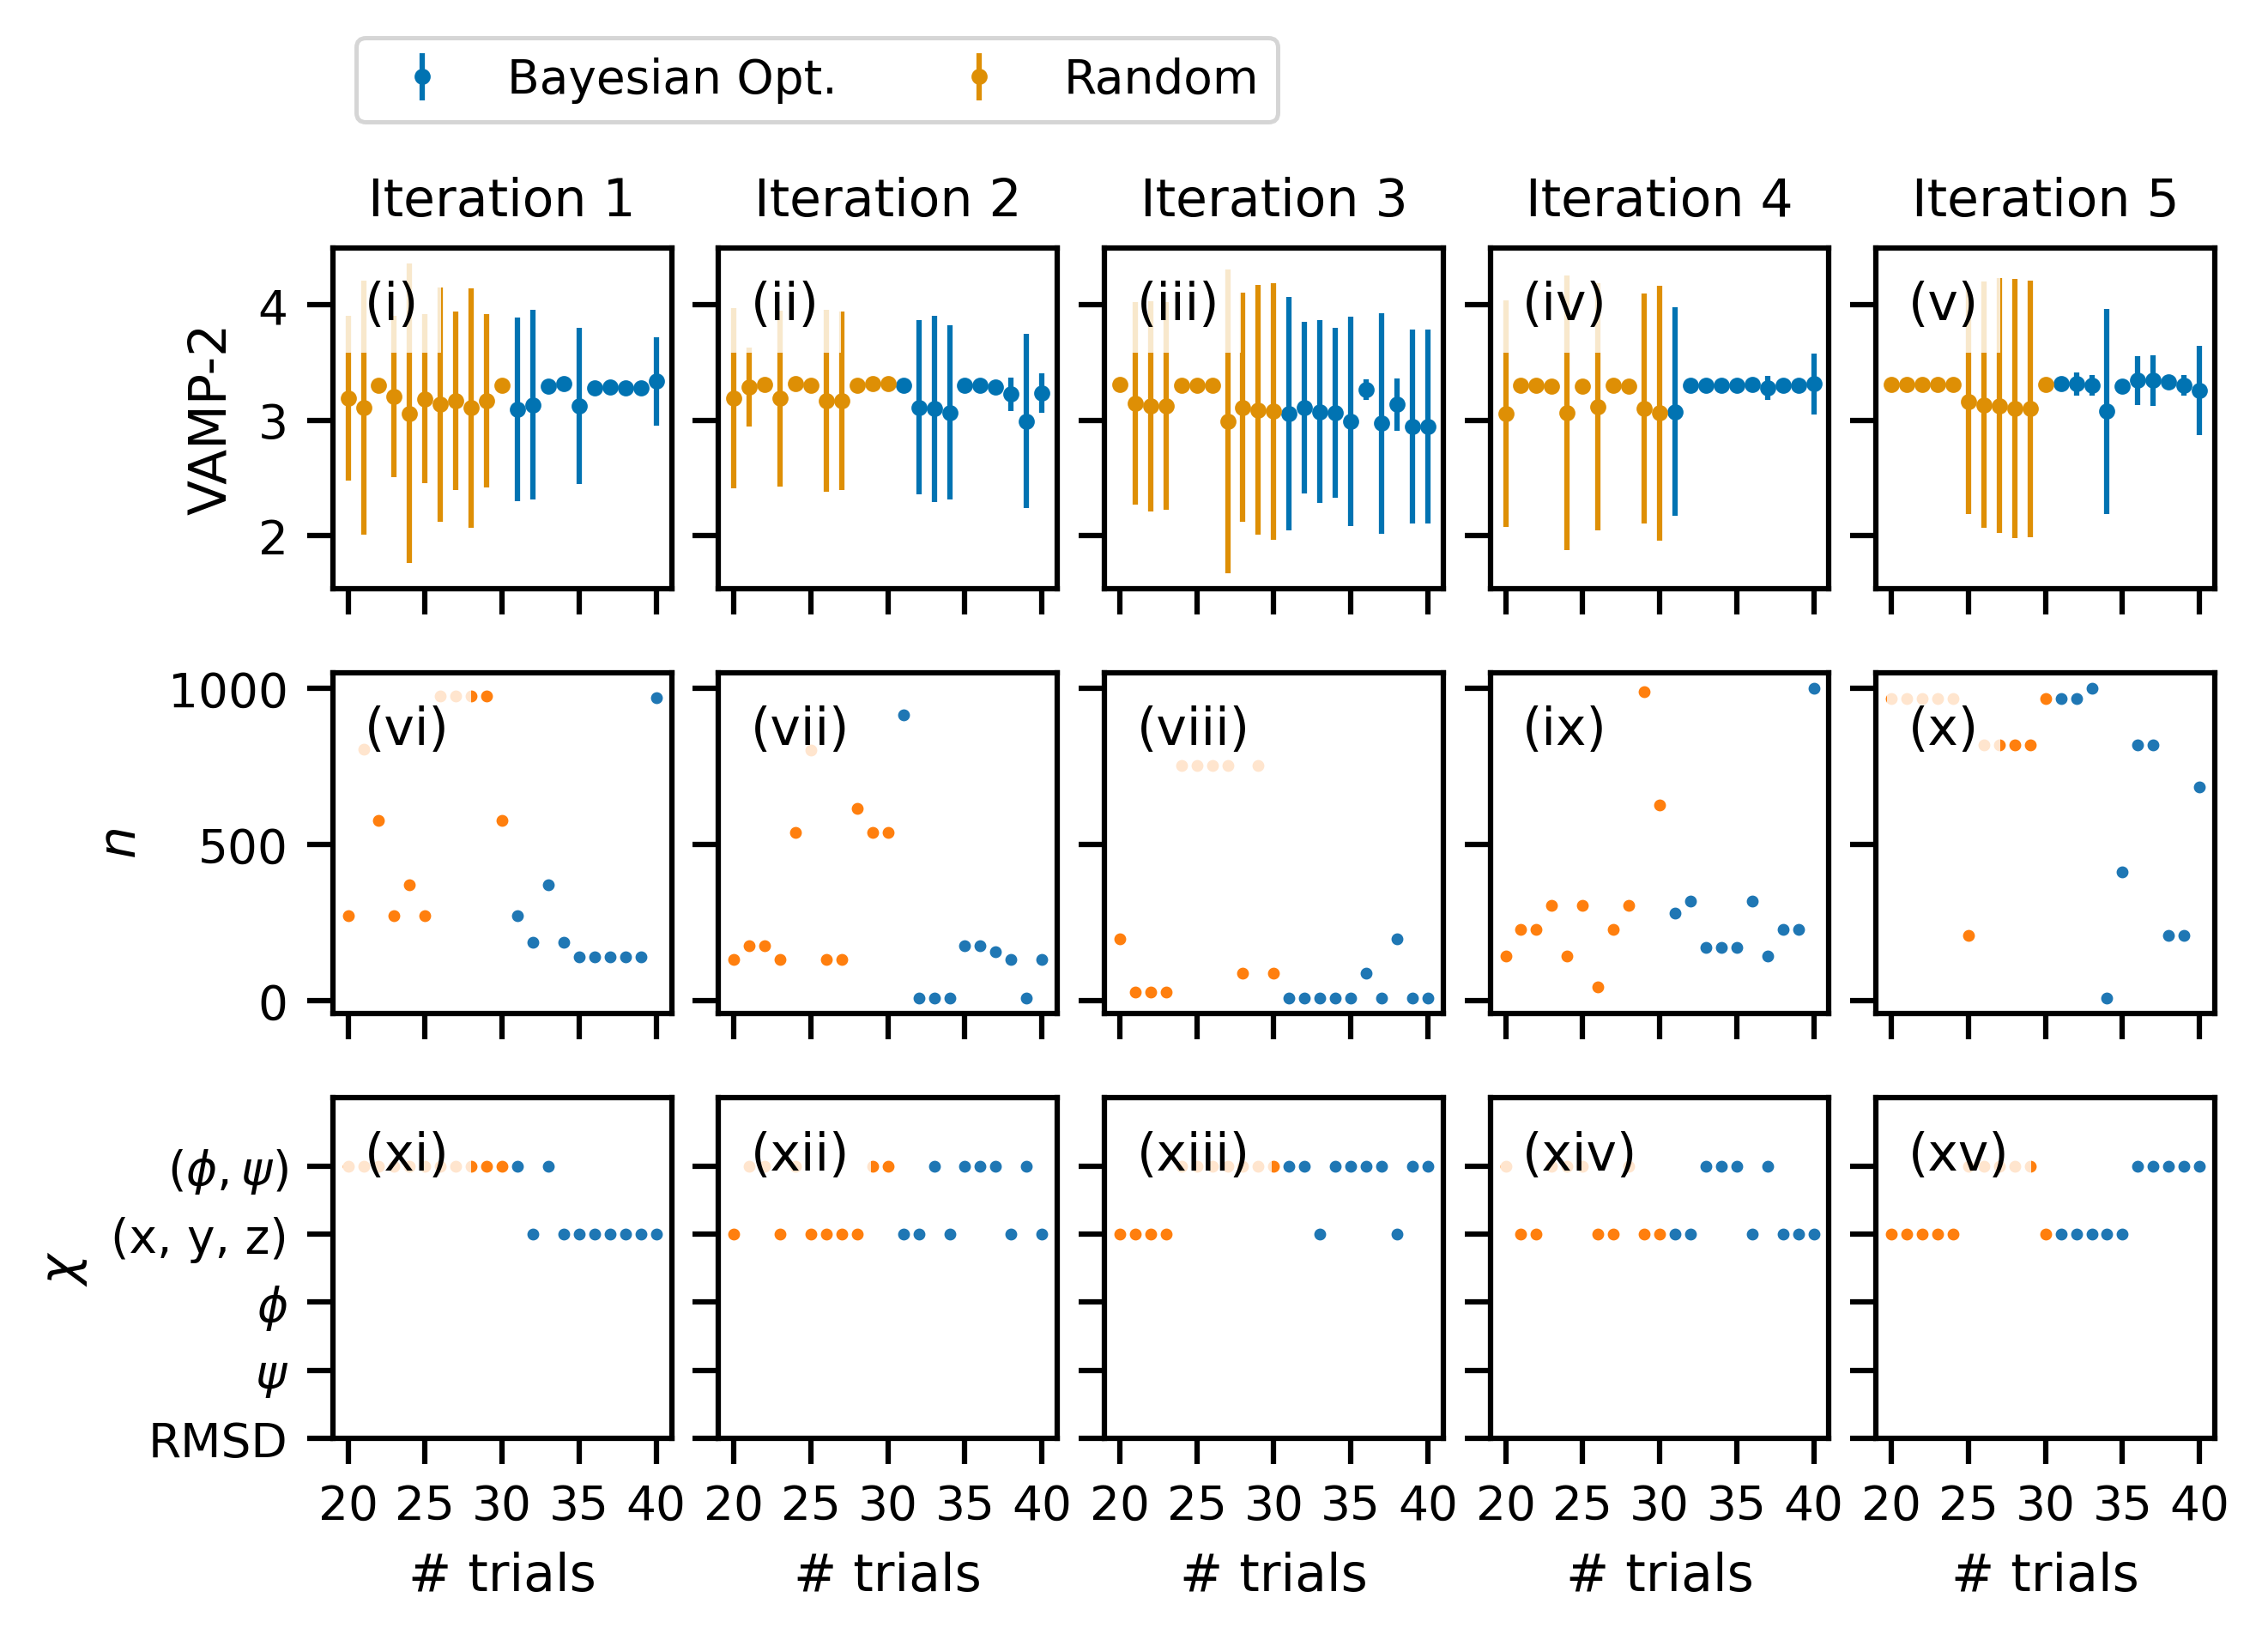
\includegraphics[width=0.7\linewidth]{chapters/msm_optimization/figures/ala1_opt_traj_start_obs_30.png}}
    
    \subtop[$N_{seed}=50$ \label{fig:ala_opt_traj_50}]{
        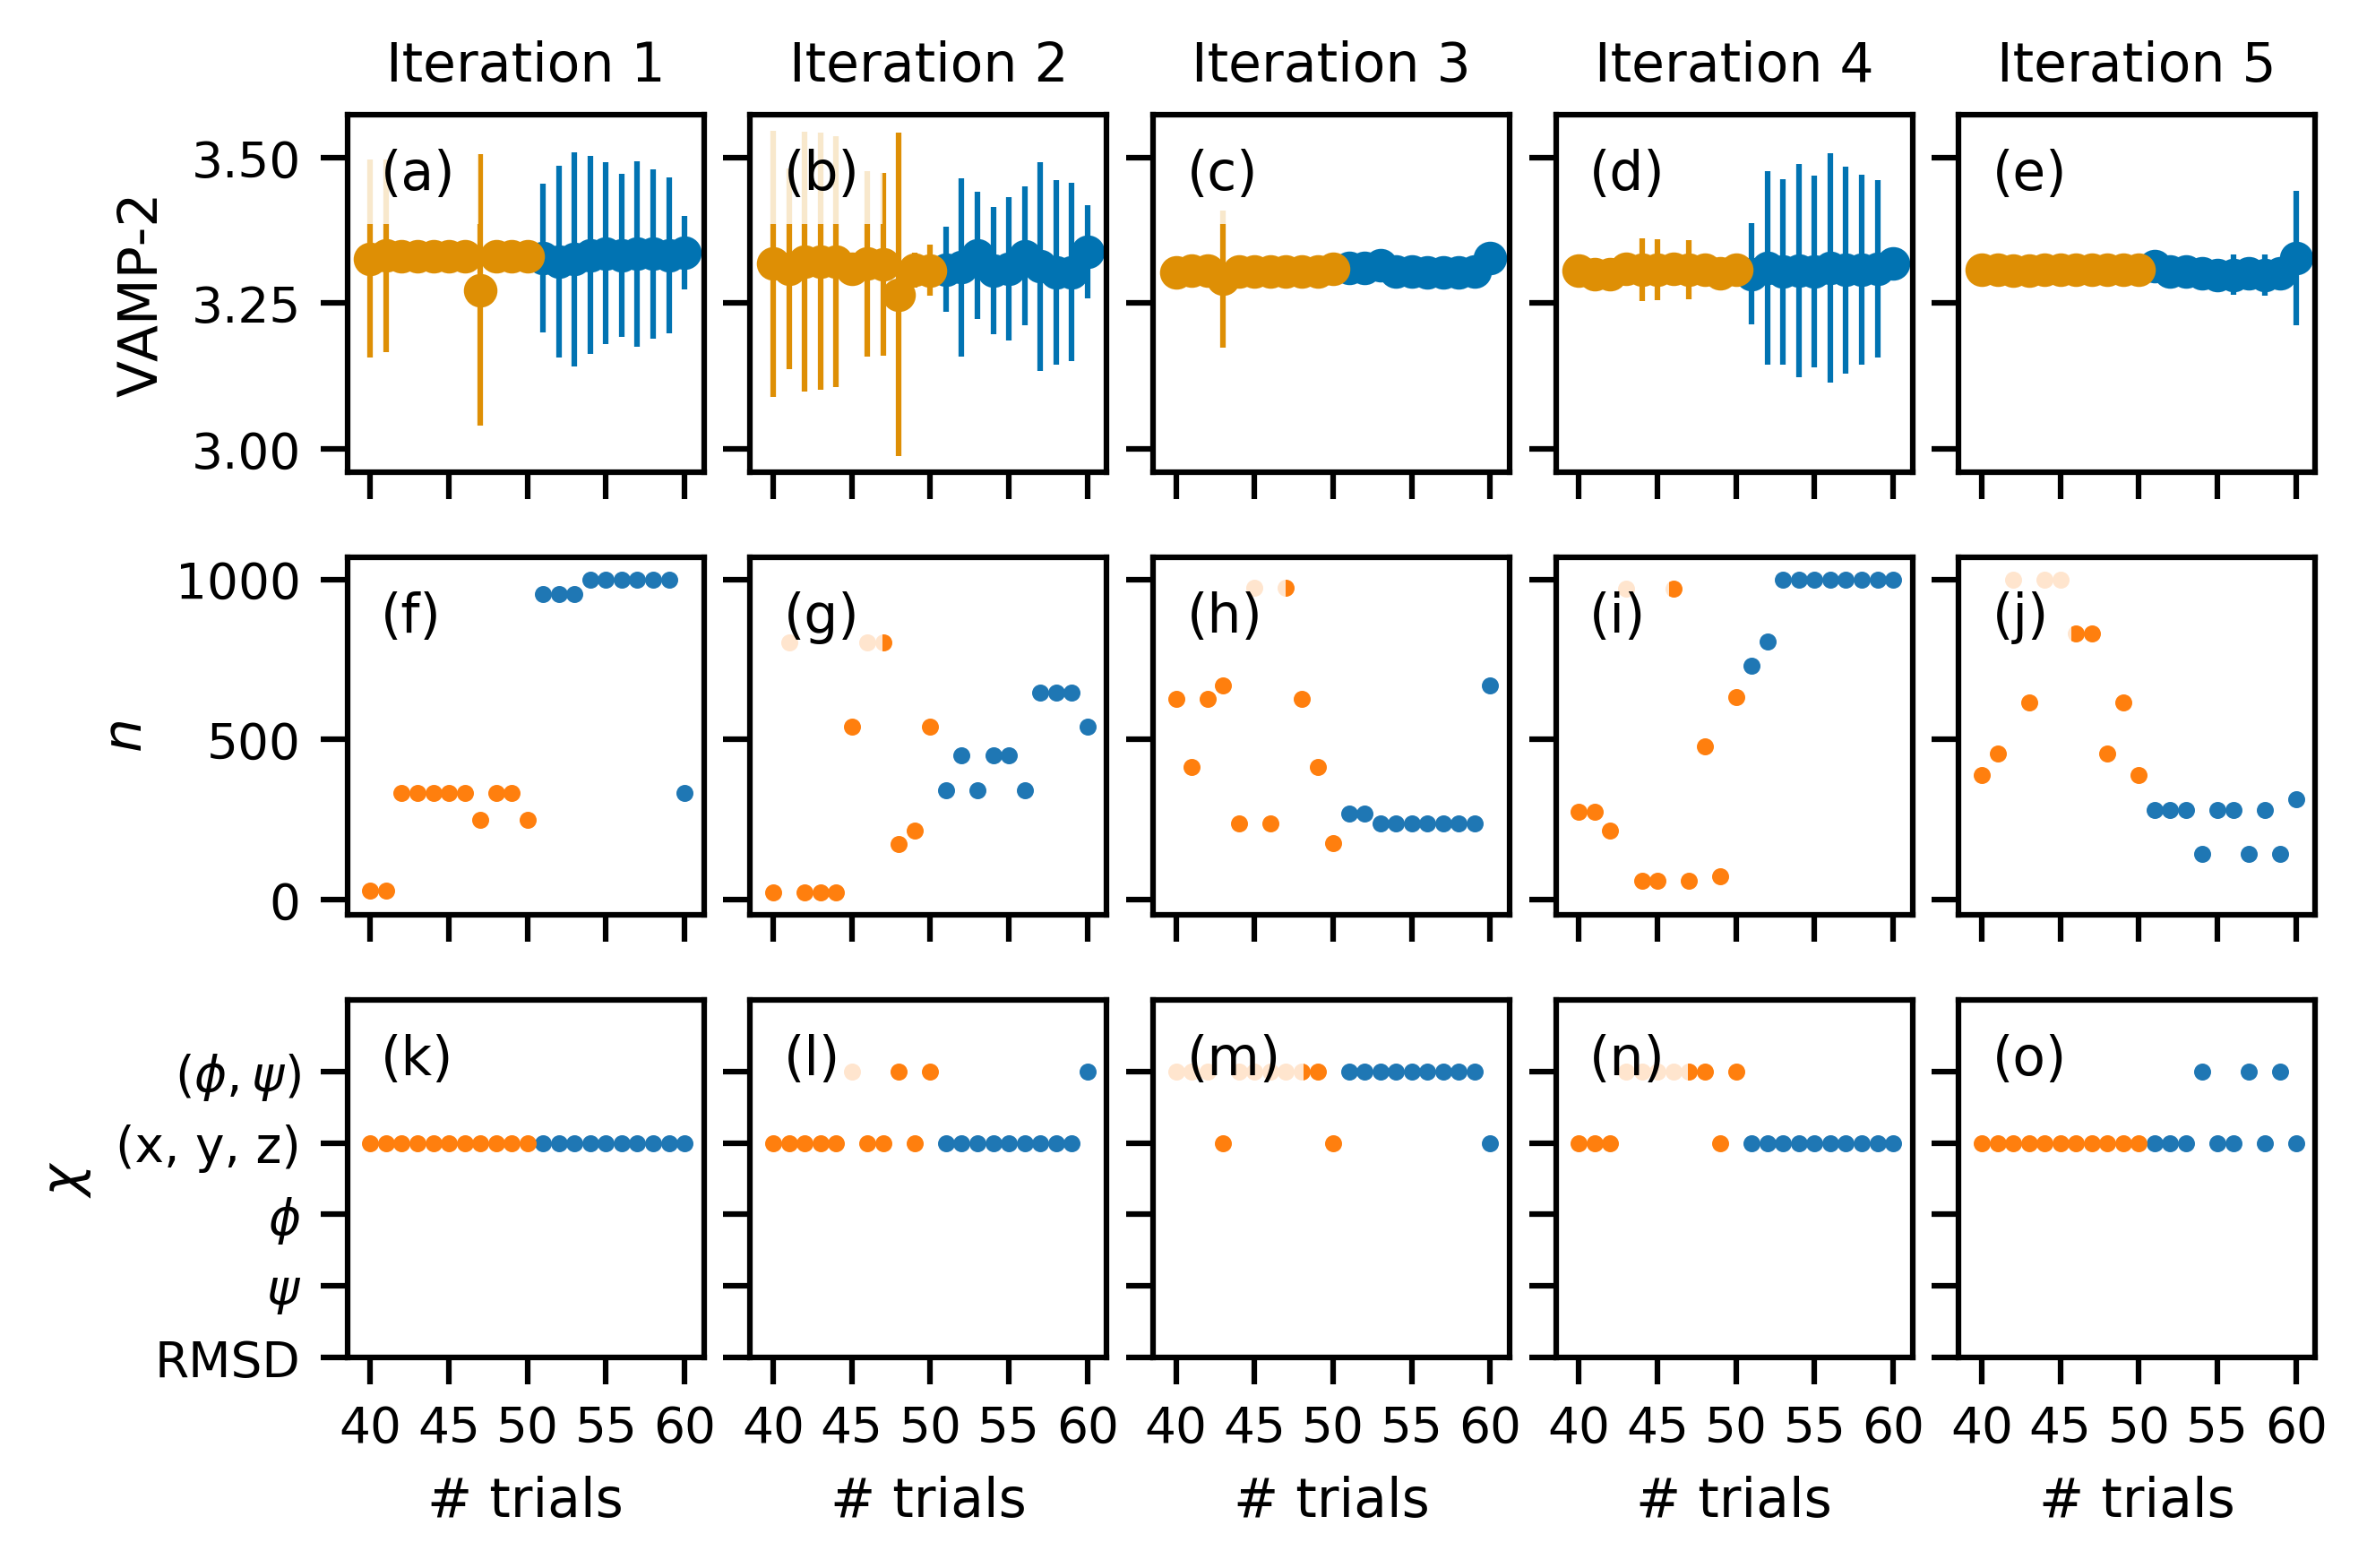
\includegraphics[width=0.7\linewidth]{chapters/msm_optimization/figures/ala1_opt_traj_start_obs_50.png}}
\end{figure}


% Optimum MSM hyper-parameters for AADH pre- and post-Bayesian optimisation (BO). Each column represents a Bayesian optimisation experiment, seeded with $N_{seed}$ randomly sampled hyper-parameter trials. Five iterations of optimisation were run with $N_{seed}=100$ (labelled $\# 1, 2$ etc.) and a single iteration optimising the response surface using all the trial data ($N_{seed}=361$). Each row is a variable or outcome with values associated with the optimum value of $\mu$ before and after the BO.


\begin{table}
    \centering
    \mycaption{Optimum MSM hyper-parameters for alanine dipeptide pre- and post- Bayesian optimisation (BO).  Each row represents a BO experiment, seeded with $N_{seed}$ randomly sampled hyper-parameters trials. Five iterations of optimisation were run with $N_{seed}=30, 50$ (labelled $\# 1, 2$ etc.). The number of optimisation steps is equal to the difference in the pre/post value of $N_{total}$.  The optimum of the response surface estimated with all the trial data ($N_{total}=500$) is included even though it was not optimised using BO. Each column is a variable or outcome with values associated with the optimum value of $\mu$ before and after the BO.  
    }
\begin{tabular}{|ll|rr|rr|rr|ll|rr|}
\hline
   &   & $N_{total}$ & & $\mu$ & & $\sigma$ & & $\chi$ &  & $n$ & \\
 $N_{seed}$  &   \#  &         Pre & Post &   Pre &  Post &      Pre &  Post &  Pre & Post & Pre & Post \\
\hline\hline
0  & 1 &         500 &      & 3.318 &       &    0.002 &       &     $(x, y, z)$ &              & 762 &      \\
\hline
30 & 1 &          30 &   40 & 3.302 & 3.338 &    0.004 & 0.192 &  $(\phi, \psi)$ &     $(x, y, z)$ & 577 &  969 \\
   & 2 &          30 &   40 & 3.318 & 3.233 &    0.005 & 0.086 &  $(\phi, \psi)$ &     $(x, y, z)$ & 540 &  133 \\
   & 3 &          30 &   40 & 3.076 & 2.947 &    0.557 & 0.420 &  $(\phi, \psi)$ &  $(\phi, \psi)$ &  88 &   10 \\
   & 4 &          30 &   40 & 3.065 & 3.315 &    0.553 & 0.132 &     $(x, y, z)$ &     $(x, y, z)$ & 627 & 1000 \\
   & 5 &          30 &   40 & 3.313 & 3.258 &    0.005 & 0.194 &     $(x, y, z)$ &  $(\phi, \psi)$ & 968 &  684 \\
   \hline
50 & 1 &          50 &   60 & 3.330 & 3.337 &    0.012 & 0.032 &     $(x, y, z)$ &     $(x, y, z)$ & 251 &  333 \\
   & 2 &          50 &   60 & 3.306 & 3.338 &    0.022 & 0.040 &  $(\phi, \psi)$ &  $(\phi, \psi)$ & 540 &  540 \\
   & 3 &          50 &   60 & 3.309 & 3.327 &    0.013 & 0.013 &     $(x, y, z)$ &     $(x, y, z)$ & 176 &  670 \\
   & 4 &          50 &   60 & 3.307 & 3.318 &    0.005 & 0.004 &  $(\phi, \psi)$ &     $(x, y, z)$ & 634 & 1000 \\
   & 5 &          50 &   60 & 3.308 & 3.327 &    0.004 & 0.058 &     $(x, y, z)$ &     $(x, y, z)$ & 390 &  314 \\
\hline
\end{tabular}

    \label{tab:ala1_best_params}
\end{table}

The maximum of the response surface \emph{at the trial values} gives the optimum hyperparameters incorporating uncertainty and making full use of all the trial information. For alanine dipeptide, the maximum of the response surface, $\mu=\num{3.318}\pm\num{0.004}$, corresponds to using the $(x, y, z)$ coordinates feature with $n=762$ cluster centers. Given its simplicity, visual inspection of the response surface (figure \ref{fig:ala1_response}) was deemed sufficient to confirm that no more sampling was necessary to locate the maximum. 

Bayesian optimisation was used to determine whether this maximum could be achieved using a smaller number of trials and to test the code written to perform the optimisation. $p=10$ steps of Bayesian optimisation was performed on five, randomly sampled, subsets of the full hyper-parameter trial data set with sizes $N_{seed}=30,50$.  The optimisation trajectories (i.e. the value of the incumbent and the associated predictors)  with $N_{seed}=30$ trials (or 15 observations-per-predictor) is shown in figure \ref{fig:ala_opt_traj_30} and with $N_{seed}=50$ (or 25 observations-per-predictor) is shown in figure \ref{fig:ala_opt_traj_50}). The $10$ steps of Bayesian optimisation are shown in blue (horizontal axis values $N_{seed} \rightarrow N_{seed}+10$) and for comparison the figure also shows, in orange, the trajectory calculated using randomly sampled trials  (horizontal axis values $N_{seed}-10 \rightarrow N_{seed}$). The input warping  and kernel function used in the response surfaces for all of the Bayesian optimisation experiments were the same as those used on the full trial data set. In principle these modelling choices should be determined independently for each data set but given the simplicity of the response surface it was deemed unnecessary. 

With $N_{seed}=30$ the incumbent trajectories of iteration 2, 3, \& 5 decreased , while for all iterations seeded with $50$ seed trials \ref{fig:ala_opt_traj} the incumbent trajectories remained constant or increased. In both cases the optimal values of $\chi$ were consistently oscillating between $(\phi, \psi)$ and $(x, y, z)$ while the optimal value of $n$ did not converge to a single value across the iterations. A value of  $N_{seed} = 50$ or $25$ observations per predictor were therefore deemed tentatively appropriate. 

There are a number of observations of the optimisation trajectories which reflect on the alanine dipeptide response surface described in section \ref{subsubsec:ala_rsm} and the usefulness of Bayesian optimisation for this system. First, the incumbent trajectories clearly show that Bayesian optimisation does not increase the value of the incumbent by a significant amount. This is a reflection of the simple nature of the response surface and the irrelevance of the number of cluster centres. Second, the response surface (in the search space domain tested) is bimodal with peaks at $\chi=(\phi, \psi)$ torsions and $(x, y, z)$ coordinates. This is reflected in the clear lack of substantive difference between the final values of $\mu$ listed in table \ref{tab:ala1_best_params}.  Third, the almost complete irrelevance of $n$ as a hyper-parameter is clearly shown in panels (f) to (j) in which $n \simeq 1000, 500 \& 100$ are arrived at with no clear difference in the value of the incumbent. Fourth, it is possible that with more optimisation steps it could be possible to arrive at the maximum of the response surface with less seed trial observations. While this is a possibility, the fact that Bayesian optimisation is an inherently serial algorithm (parallel variants which sample the acquisition function rather than optimise do exist []), while random sampling is embarrassingly parallel, it was considered more wall-time efficient (if not CPU-time efficient) to err on the side of more random seed trial data and less optimisation steps. 

\subsection{Aromatic Amine Dehydrogenase}\label{subsec:aadh}
Having explored the use of response surfaces and Bayesian optimisation in the well known alanine dipeptide system with a two-dimensional hyper-parameter space. These techniques were applied to the unknown case of the active site of AADH. 

[TM: give summary of what's coming next]

\subsubsection{Response surface}\label{subsubsec:aadh_rsm}

\begin{figure}[p]
    \centering
    \mycaption{The $\operatorname{VAMP-2}$ scores of the hyperparameter trials for MSMs of AADH. The test response, $f^{test}=f\left(\chi, \tau, m, n; \mathbf{X}^{test}\right)$, is shown in blue, for (a) the $\phi, \psi, \chi$ torsions, (c) all distances between heavy atoms, (e) alpha-Carbon contact distances, (g) heavy atom contact distances, (i) root mean square deviation of heavy atoms. The difference between $f^{train}$ and $f^{test}$ is shown in orange for (b) the the $\phi, \psi, \chi$ torsions and so on. The horizontal axis is the rank of the trial according to the test score. Each trial was scored with $20$ iterations of 50:50 shuffle split cross-validation. The error bars represent the 25th and 75th quantiles of the cross-validation folds. The features are ordered according to the mean of the their test scores.}
    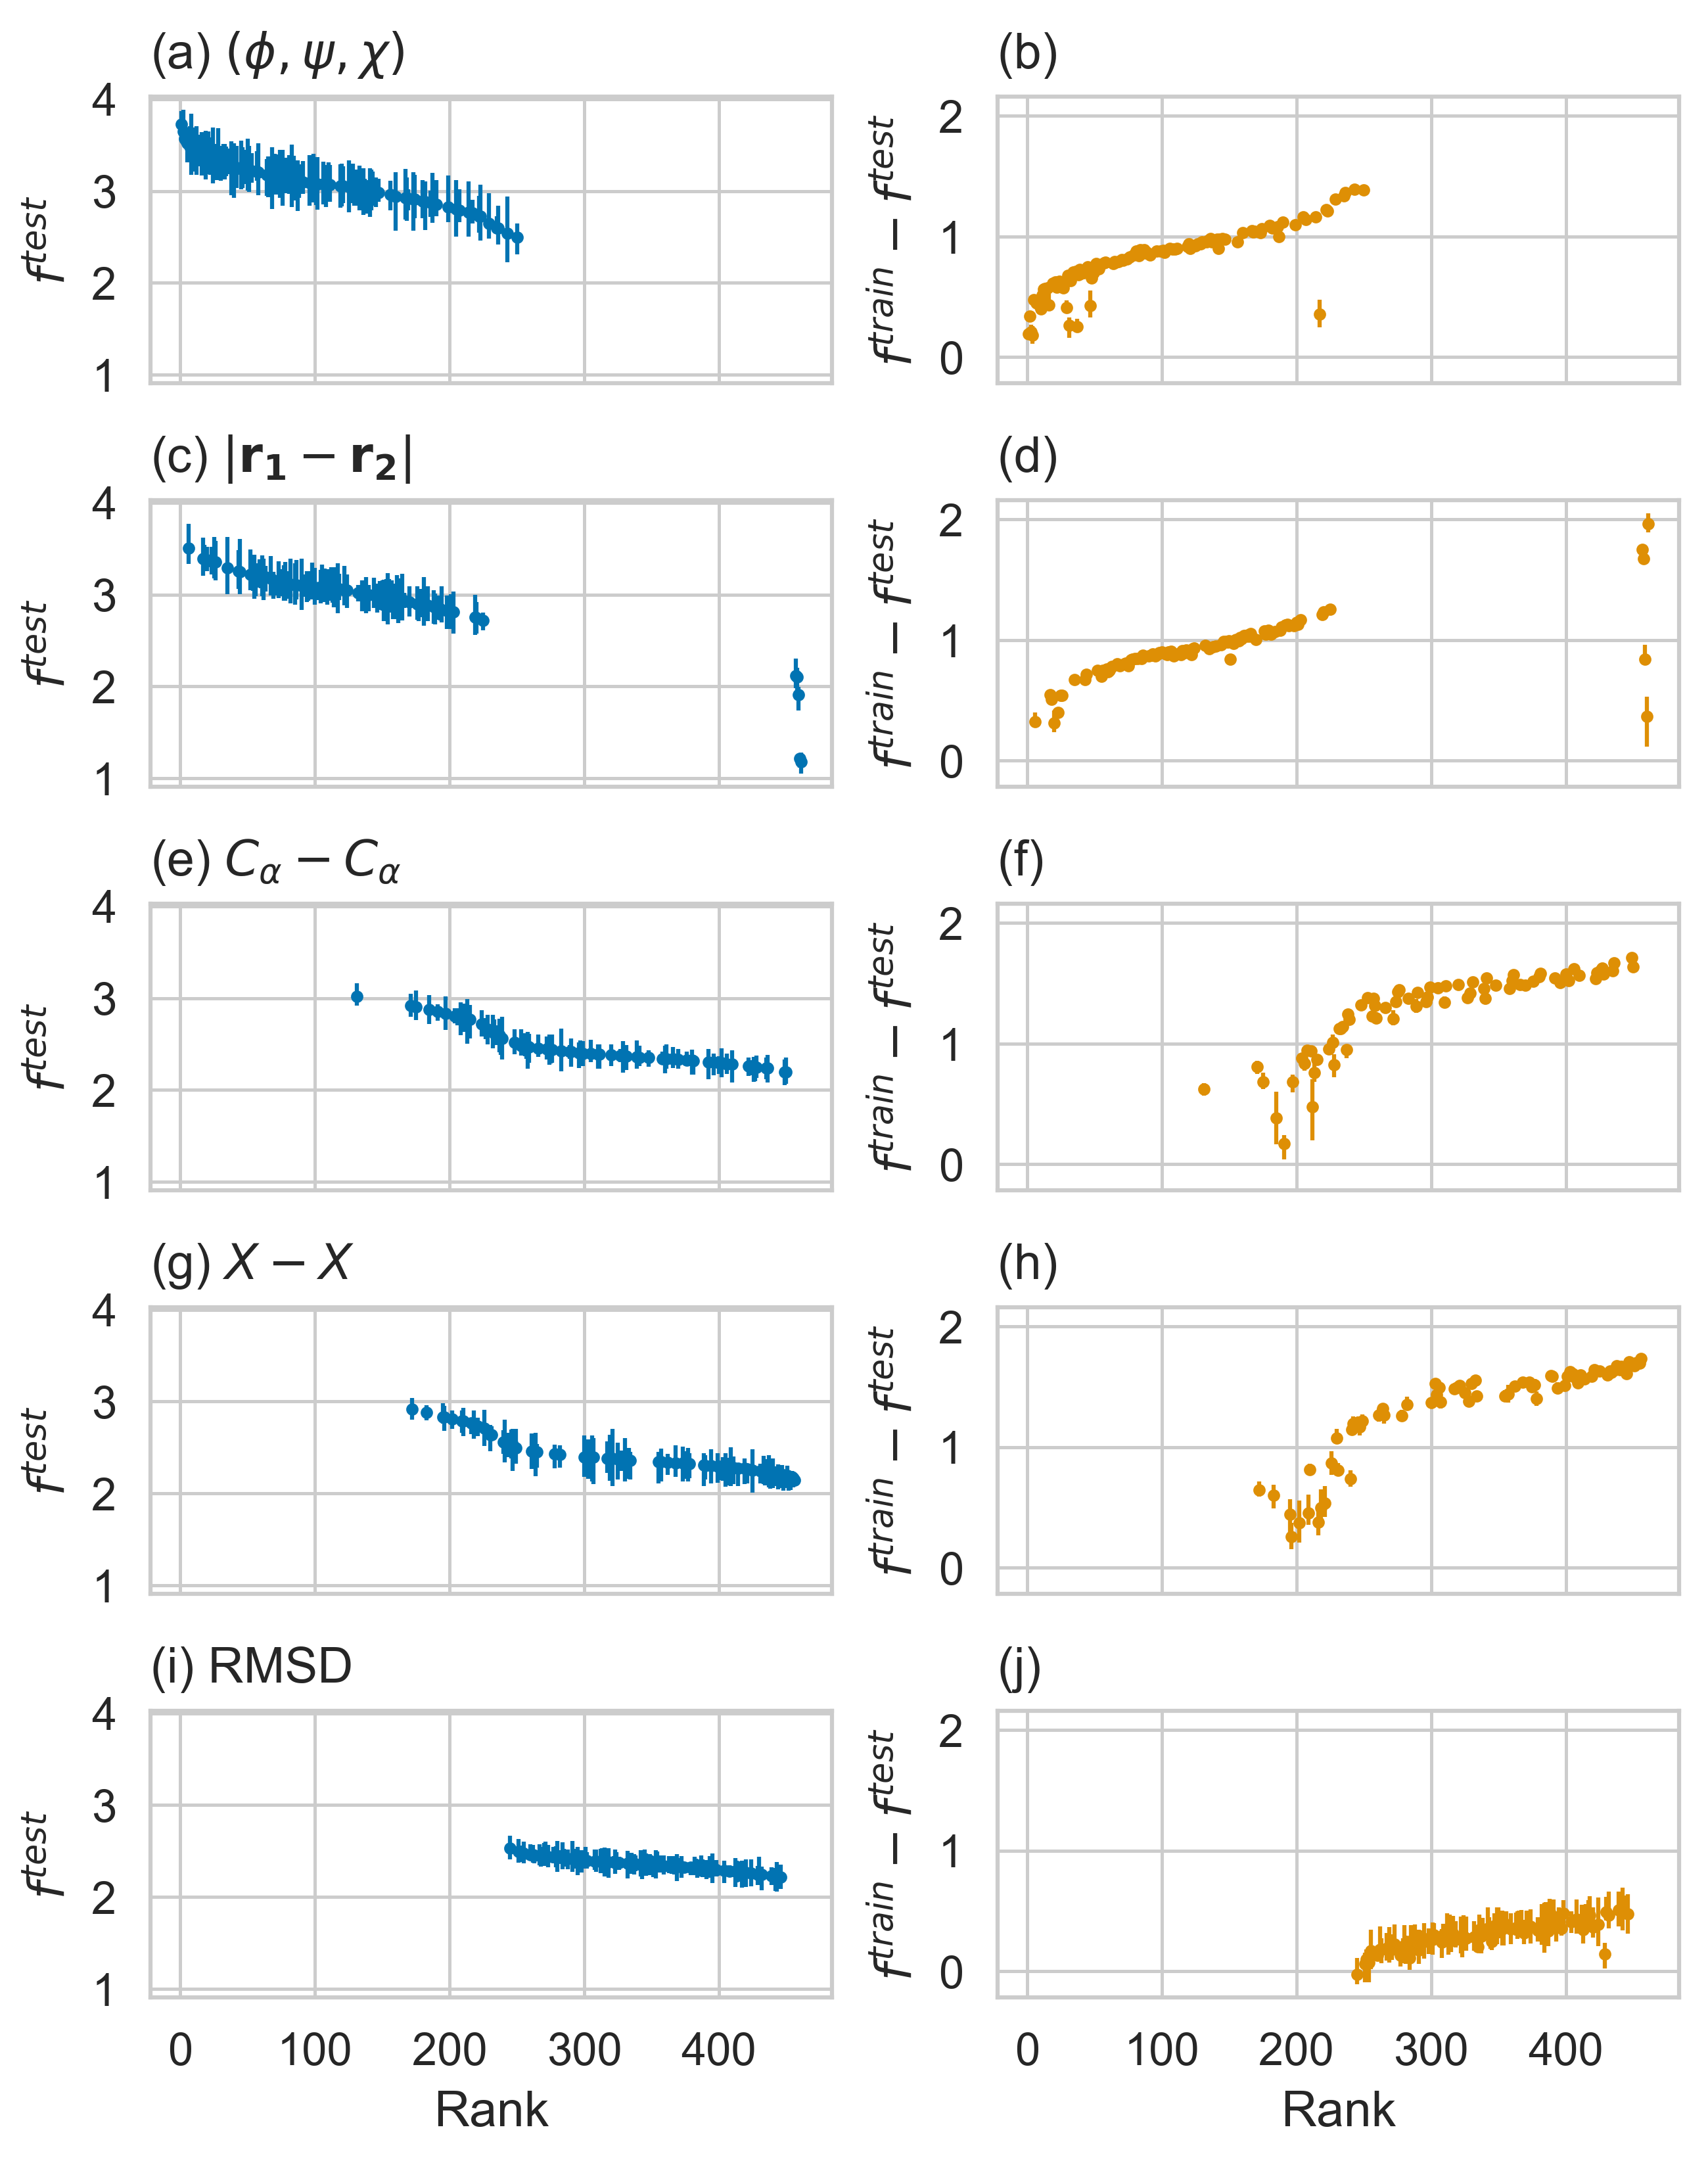
\includegraphics[width=0.8\textwidth]{chapters/msm_optimization/figures/aadh_train_test_results.png}
    \label{fig:aad_train_test}
\end{figure}

The mean MSM response for the randomly sampled hyper-parameter trials are shown in  figure \ref{fig:aad_train_test} with the test response shown in blue and the difference between the training and test response shown in orange.  The panels correspond to the value $\chi$ and are ordered according to their average of the test responses. The horizontal axis is the rank of the trial determined by their test response. There is clear range of response values in the range $2 < \operatorname{VAMP-2} < 4$ with the $(\phi, \psi, \chi)$ torsions  (panel (a)) and the interatomic distances feature ( $\left|\mathbf{r}_{1}-\mathbf{r}_{2}\right|$) (panel (c)) both performing the best out of the five features. 

In contrast to the case of alanine dipeptide, all features show a marked degree of over-fitting $\Delta f$. However, within each feature there are combinations of the remaining hyper-parameters for which $\Delta f=0$ implying that it is possible to create a consistent picture of relaxation processes which generalize well for each feature. The response of the $(\phi, \psi, \chi)$ feature  approaches the maximum response of $VAMP-2 = 4$ for the highest ranked trials, indicating the possibility of the three slow relaxation processes. 

\begin{figure}
    \centering
    \mycaption{[TM: label with Pearson R for each panel?] Goodness of fit for the response surface of AADH conditional on each feature. The horizontal axis ($y$) are the observed trial values and the vertical axis is the mean response ($f(\mathbf{x})$). The error bars are $\pm 2\sigma$ where $\sigma$ is the standard deviation of the response surface including the noise term $\sigma_n$.}
    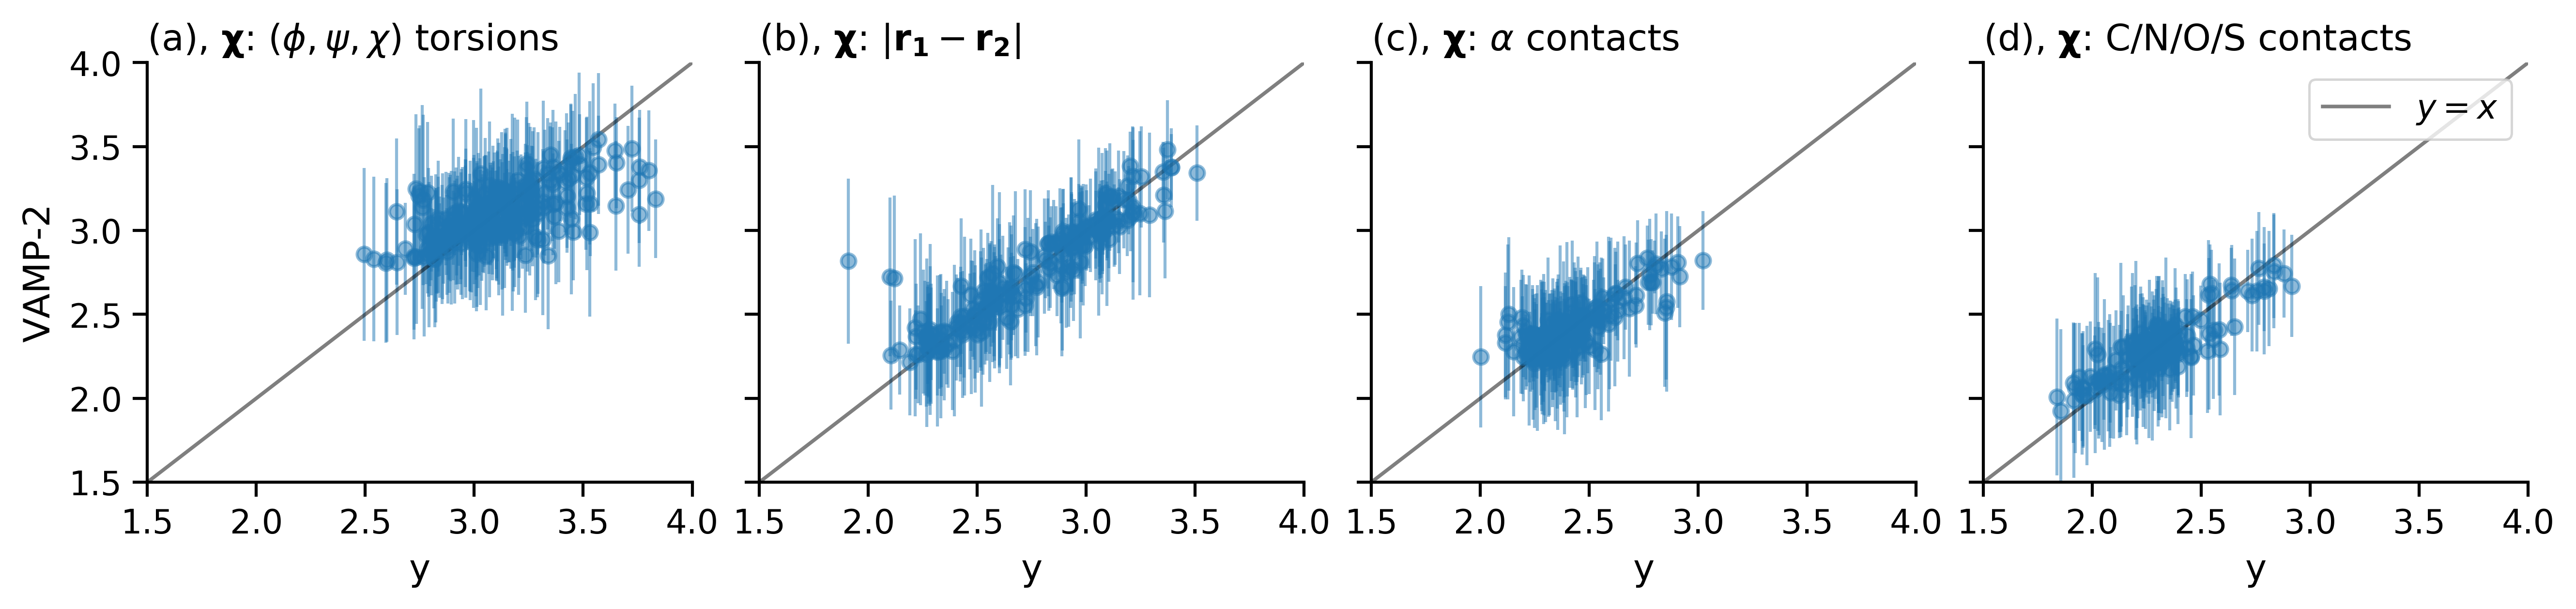
\includegraphics[width=0.8\textwidth]{chapters/msm_optimization/figures/aadh_response_surface_fit_d.png}
    
    \label{fig:aadh_rsm_fit}
\end{figure}

The response surface as a function of the feature, $\chi$, TICA lag time, $\tau$, number of TICA components retains $m$, and the number of cluster centres, $n$ was estimated with a GP. The RMSD feature was left out of the response surface because the $\tau$ and $m$ hyper-parameters do not apply, creating a \emph{conditional} search space [] which  poses problems GP although there are attempts to mitigate this []. While this is a problem in general for this method, the poor performance of RMSD as a feature both here and in alanine dipeptide mean that this will not affect finding the optimum hyper-parameters. 

[TM: how are kernel and input warping chosen?] Model selection on the kernel and input warping revealed an exponential kernel (equation \ref{eqn:kern_exp}) and a linear input transformation for $\tau, m$ and $n$ were most appropriate, with an MSLL of $-0.01298$ and a SMSE of $0.3087$ (see table \ref{tab:aadh_rsm_metrics_all_data} for the other models' selection metrics). A more intuitive assessment of the fit of the can be found in figure  \ref{fig:aadh_rsm_fit} which shows the observed and predicted values for each feature. There is clearly a good fit for all the features except for the $(\phi, \psi, \chi)$ torsions where the predicted values are slightly under/over estimated for the highest/lowest values with this feature. This creates the possibility of a false bimodal response surface which must be checked when determining the optimal hyper-parameters.  The relatively poor fit on this feature is likely due to the fully multiplicative nature of the kernel. More flexible kernels (as discussed in e.g. \cite{duvenaud2011additive}) which model lower order interactions may be able to overcome this problem. 

\begin{figure}
    \centering
    \mycaption{The relevance of the hyper-parameters of AADH. The distribution of the parameters of the response surface were estimated using MCMC. The relevance of the features (levels of $\chi$) are shown in blue, labelled `Feature'. The relevance of the the other hyper-parameters are shown in orange, labelled `Other'.}
    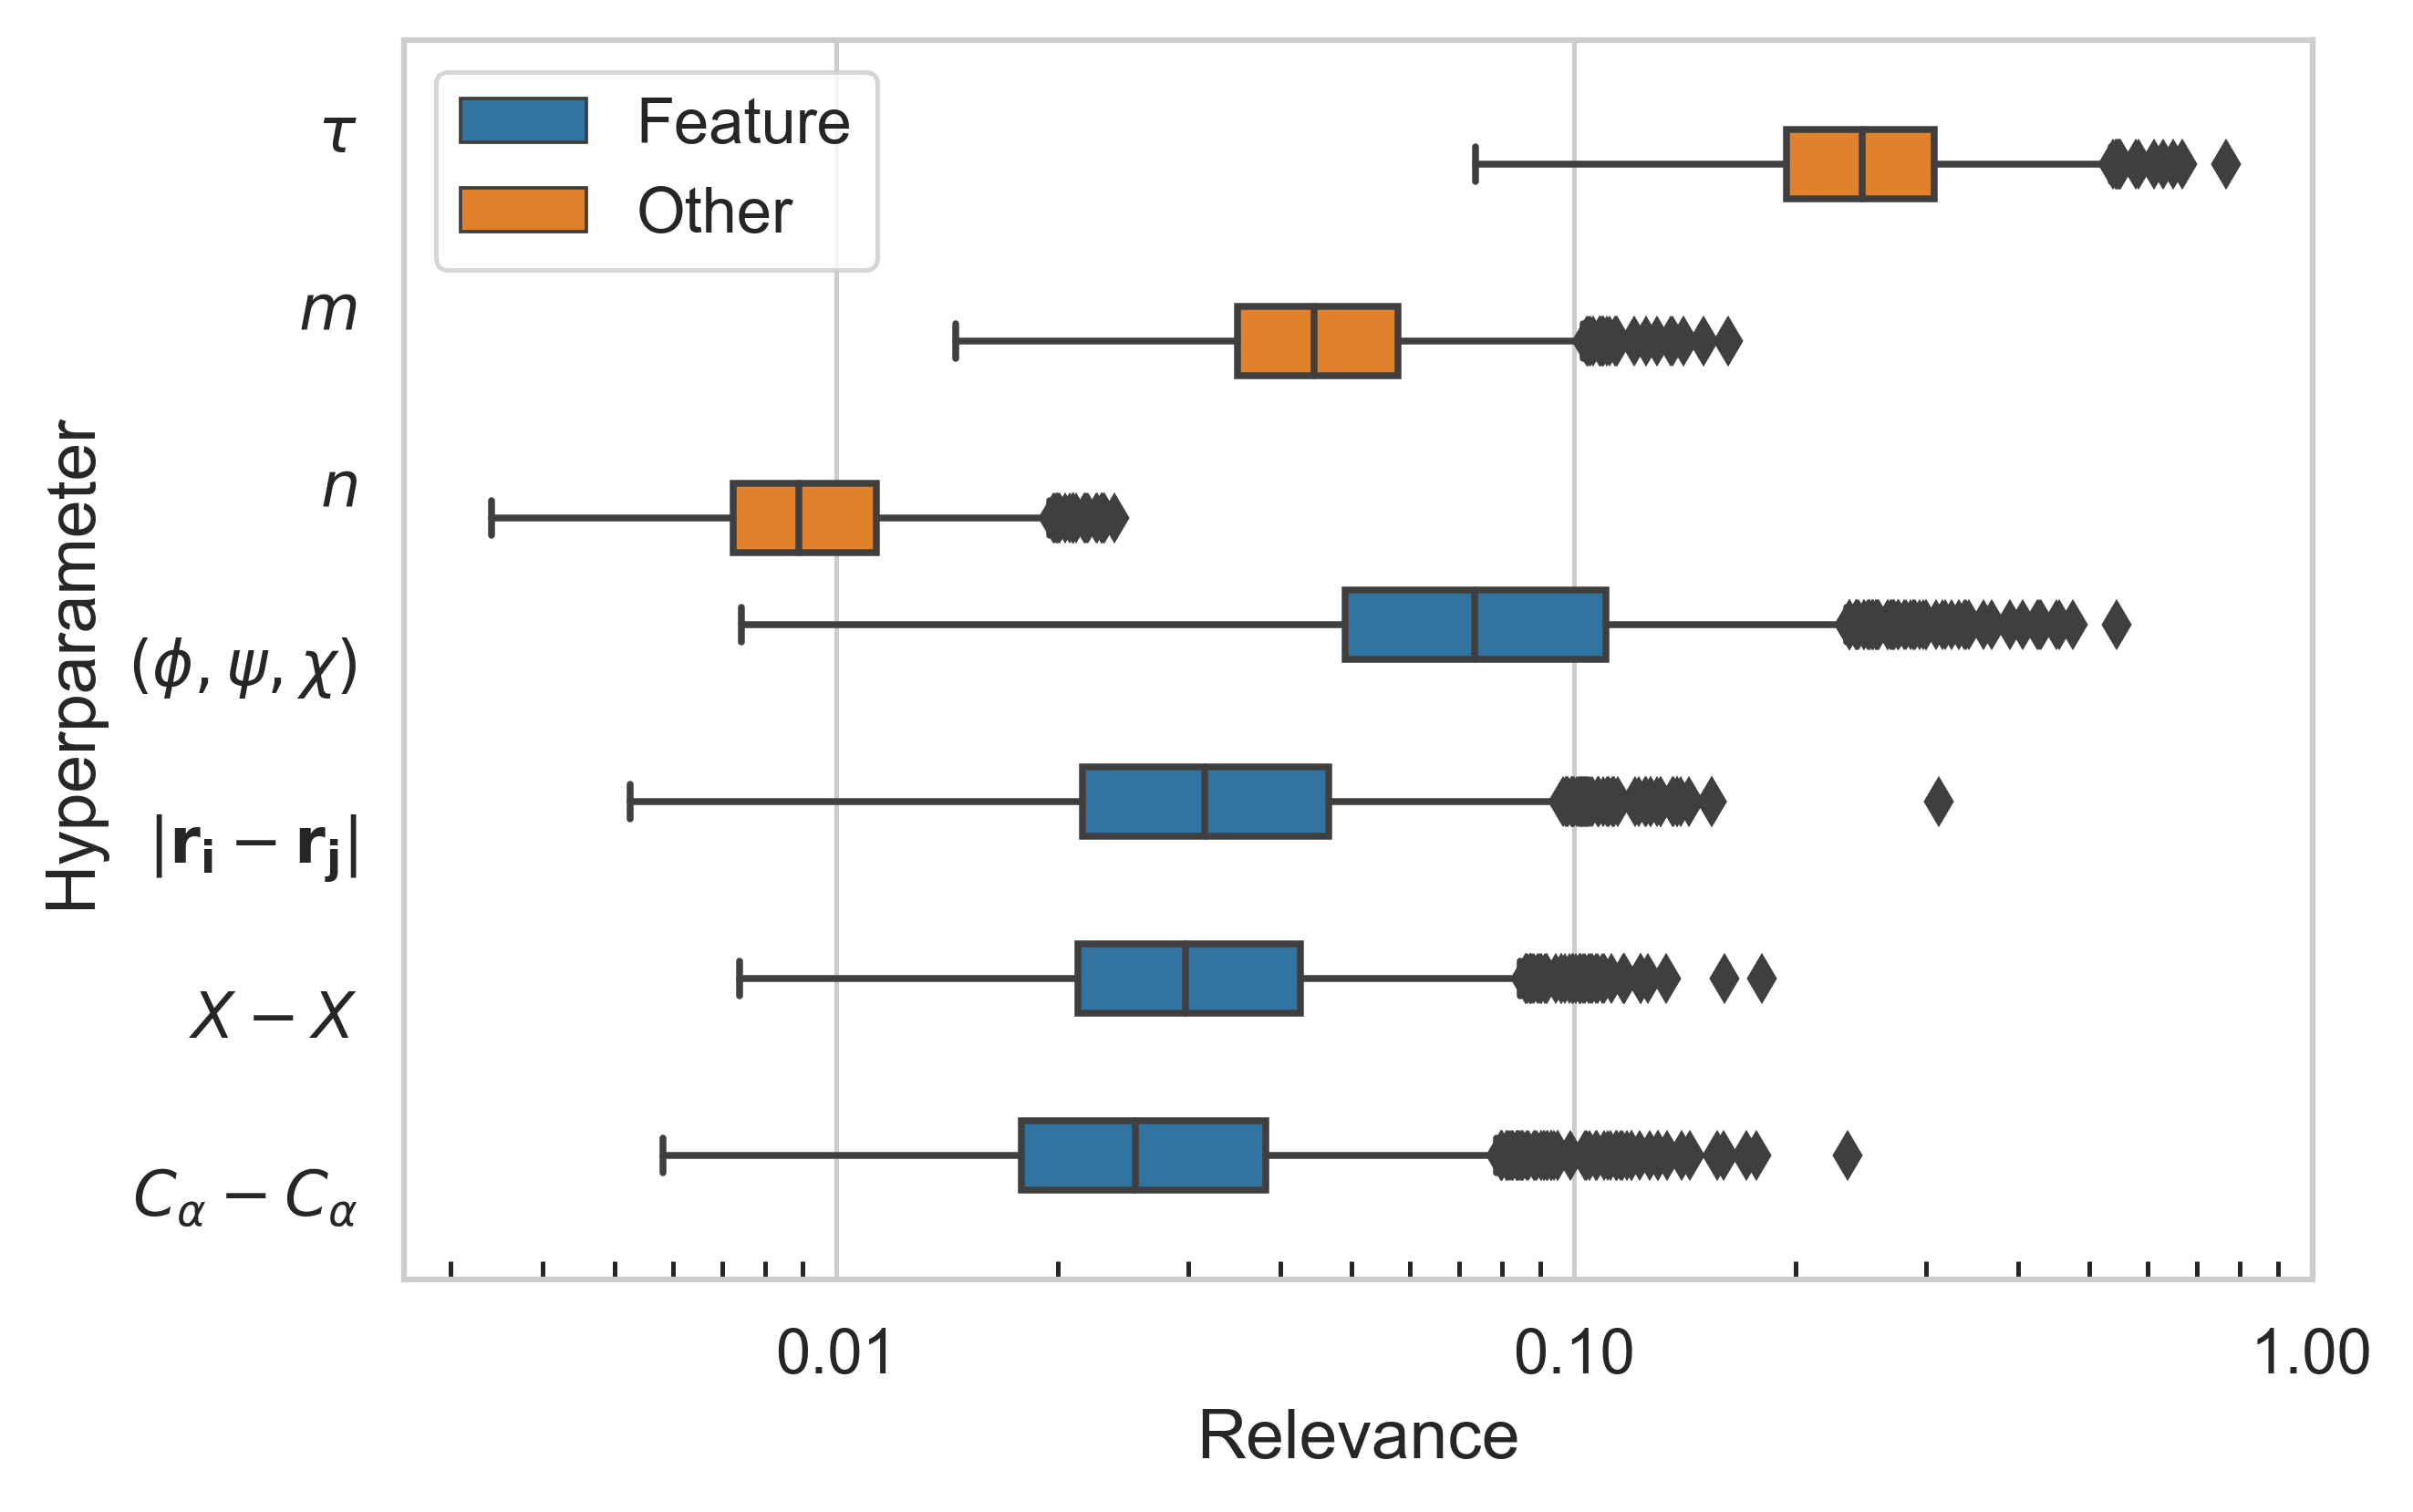
\includegraphics[width=0.8\textwidth]{chapters/msm_optimization/figures/AADH_relevance_d.png}
    \label{fig:aadh_relevance}
\end{figure}

\begin{table}
    \centering
    \mycaption{Median and $\SI{95}{\percent}$ credible intervals for the kernel hyper-parameters of the AADH response surface estimated using MCMC. The length-scale parameters in equation \ref{eqn:kernel_form} are re-written here as relevances.}
    \begin{tabular}{|l|r|l|}
    \hline
                             Hyper-parameter &  Median &     (95\% C.I.) \\
    \hline\hline
                    $R_{(\phi, \psi, \chi)}$ &   0.073 &  (0.021-0.248) \\
     $R_{|\mathbf{r_{1}} - \mathbf{r_{2}}|}$ &   0.032 &  (0.012-0.098) \\
                 $R_{C_{\alpha}-C_{\alpha}}$ &   0.025 &  (0.009-0.084) \\
                                   $R_{X-X}$ &   0.030 &  (0.012-0.083) \\
                                  $R_{\tau}$ &   0.246 &  (0.126-0.474) \\
                                     $R_{m}$ &   0.044 &  (0.022-0.095) \\
                                     $R_{n}$ &   0.009 &  (0.005-0.018) \\
                                      $\eta$ &   1.540 &  (1.117-2.154) \\
                                  $\sigma_n$ &   0.011 &  (0.001-0.035) \\
    \hline
    \end{tabular}
    \label{tab:aadh_rel}
\end{table}

The multidimensional nature of the response surface poses problems for visualisation and for understanding the interaction between the hyper-parameters in determining the response. However, calculating the hyper-parameter relevance can help by suggesting the displayed granularity of the inputs. Figure \ref{fig:aadh_relevance} shows the posterior distribution of relevance for the features (blue) and the remaining hyper-parameters (orange). The median and $\SI{95}{\percent}$ credible intervals are tabulated in table \ref{tab:aadh_rel}. 

Figure \ref{fig:aadh_rsm} shows  a projection of the response surface, $f(\mathbf{x};\mathcal{D}_{361})$, informed by the relevance. $\tau$ and $m$ are the two highest relevance hyper-parameters ($R_{\tau} = 0.246 (0.126-0.474)$, $R_{m} = 0.044 (0.022-0.095)$) so the response surface is shown as a 2D heat map with $\tau$ on the vertical and $m$ on the horizontal axis. Only odd values of $m$ are shown given the slightly lower relevance of this feature. The number of cluster features is, like the case of alanine dipeptide, the lowest relevance hyper-parameter ($R_{n} = 0.009 (0.005-0.018)$ and so heat maps for only two value of $n$ are shown: the value at the maximum of the response surface ($n=207$ although the value displayed is rounded to $210$) and $n=1000$. With only four features, it is  simple to show the response surface for each of them. With a larger number of features, displaying the high relevance features and \emph{only one} of the low relevance features would be sufficient. This is clearly borne out with this surface - the two lower relevance features, the contact distances, are very similar and including both in the visualisation is redundant. However, as all features have absolutely low relevance ($R<1$) then their response surfaces are expected to be similar. The maximum of the response surface is shown highlighted in white, occurs at $\mathbf{x}=\left(\chi=(\phi, \psi, \chi), \tau = \SI{12.5}{\nano\second}, m=1, n=207\right)$ with a value of $\mu=3.54 3\pm 0.396$. The features of this response surface will be discussed in the context of sensitivity analysis in later sections. 

\begin{figure}[p]
    \centering
    \mycaption{The response surface of AADH using the unoptimised hyper-parameter trial data set. For each feature two heat maps are shown for $n=210, 1000$ with $\tau$ on the vertical axis and $m$ on the horizontal axis: for the dihedrals feature panel (a) shows the heat map for $n=210$  and panel (b) shows the heat map for $n=1000$ and similarly for the remaining features. The white star denotes the approximate location of the maximum of the surface, the true maximum occurs at $\tau=\SI{12.5}{\nano\second}, m=1, n=207$  The value of the response surface denoted by the color (lighter implies higher values) and with the text annotations. }
    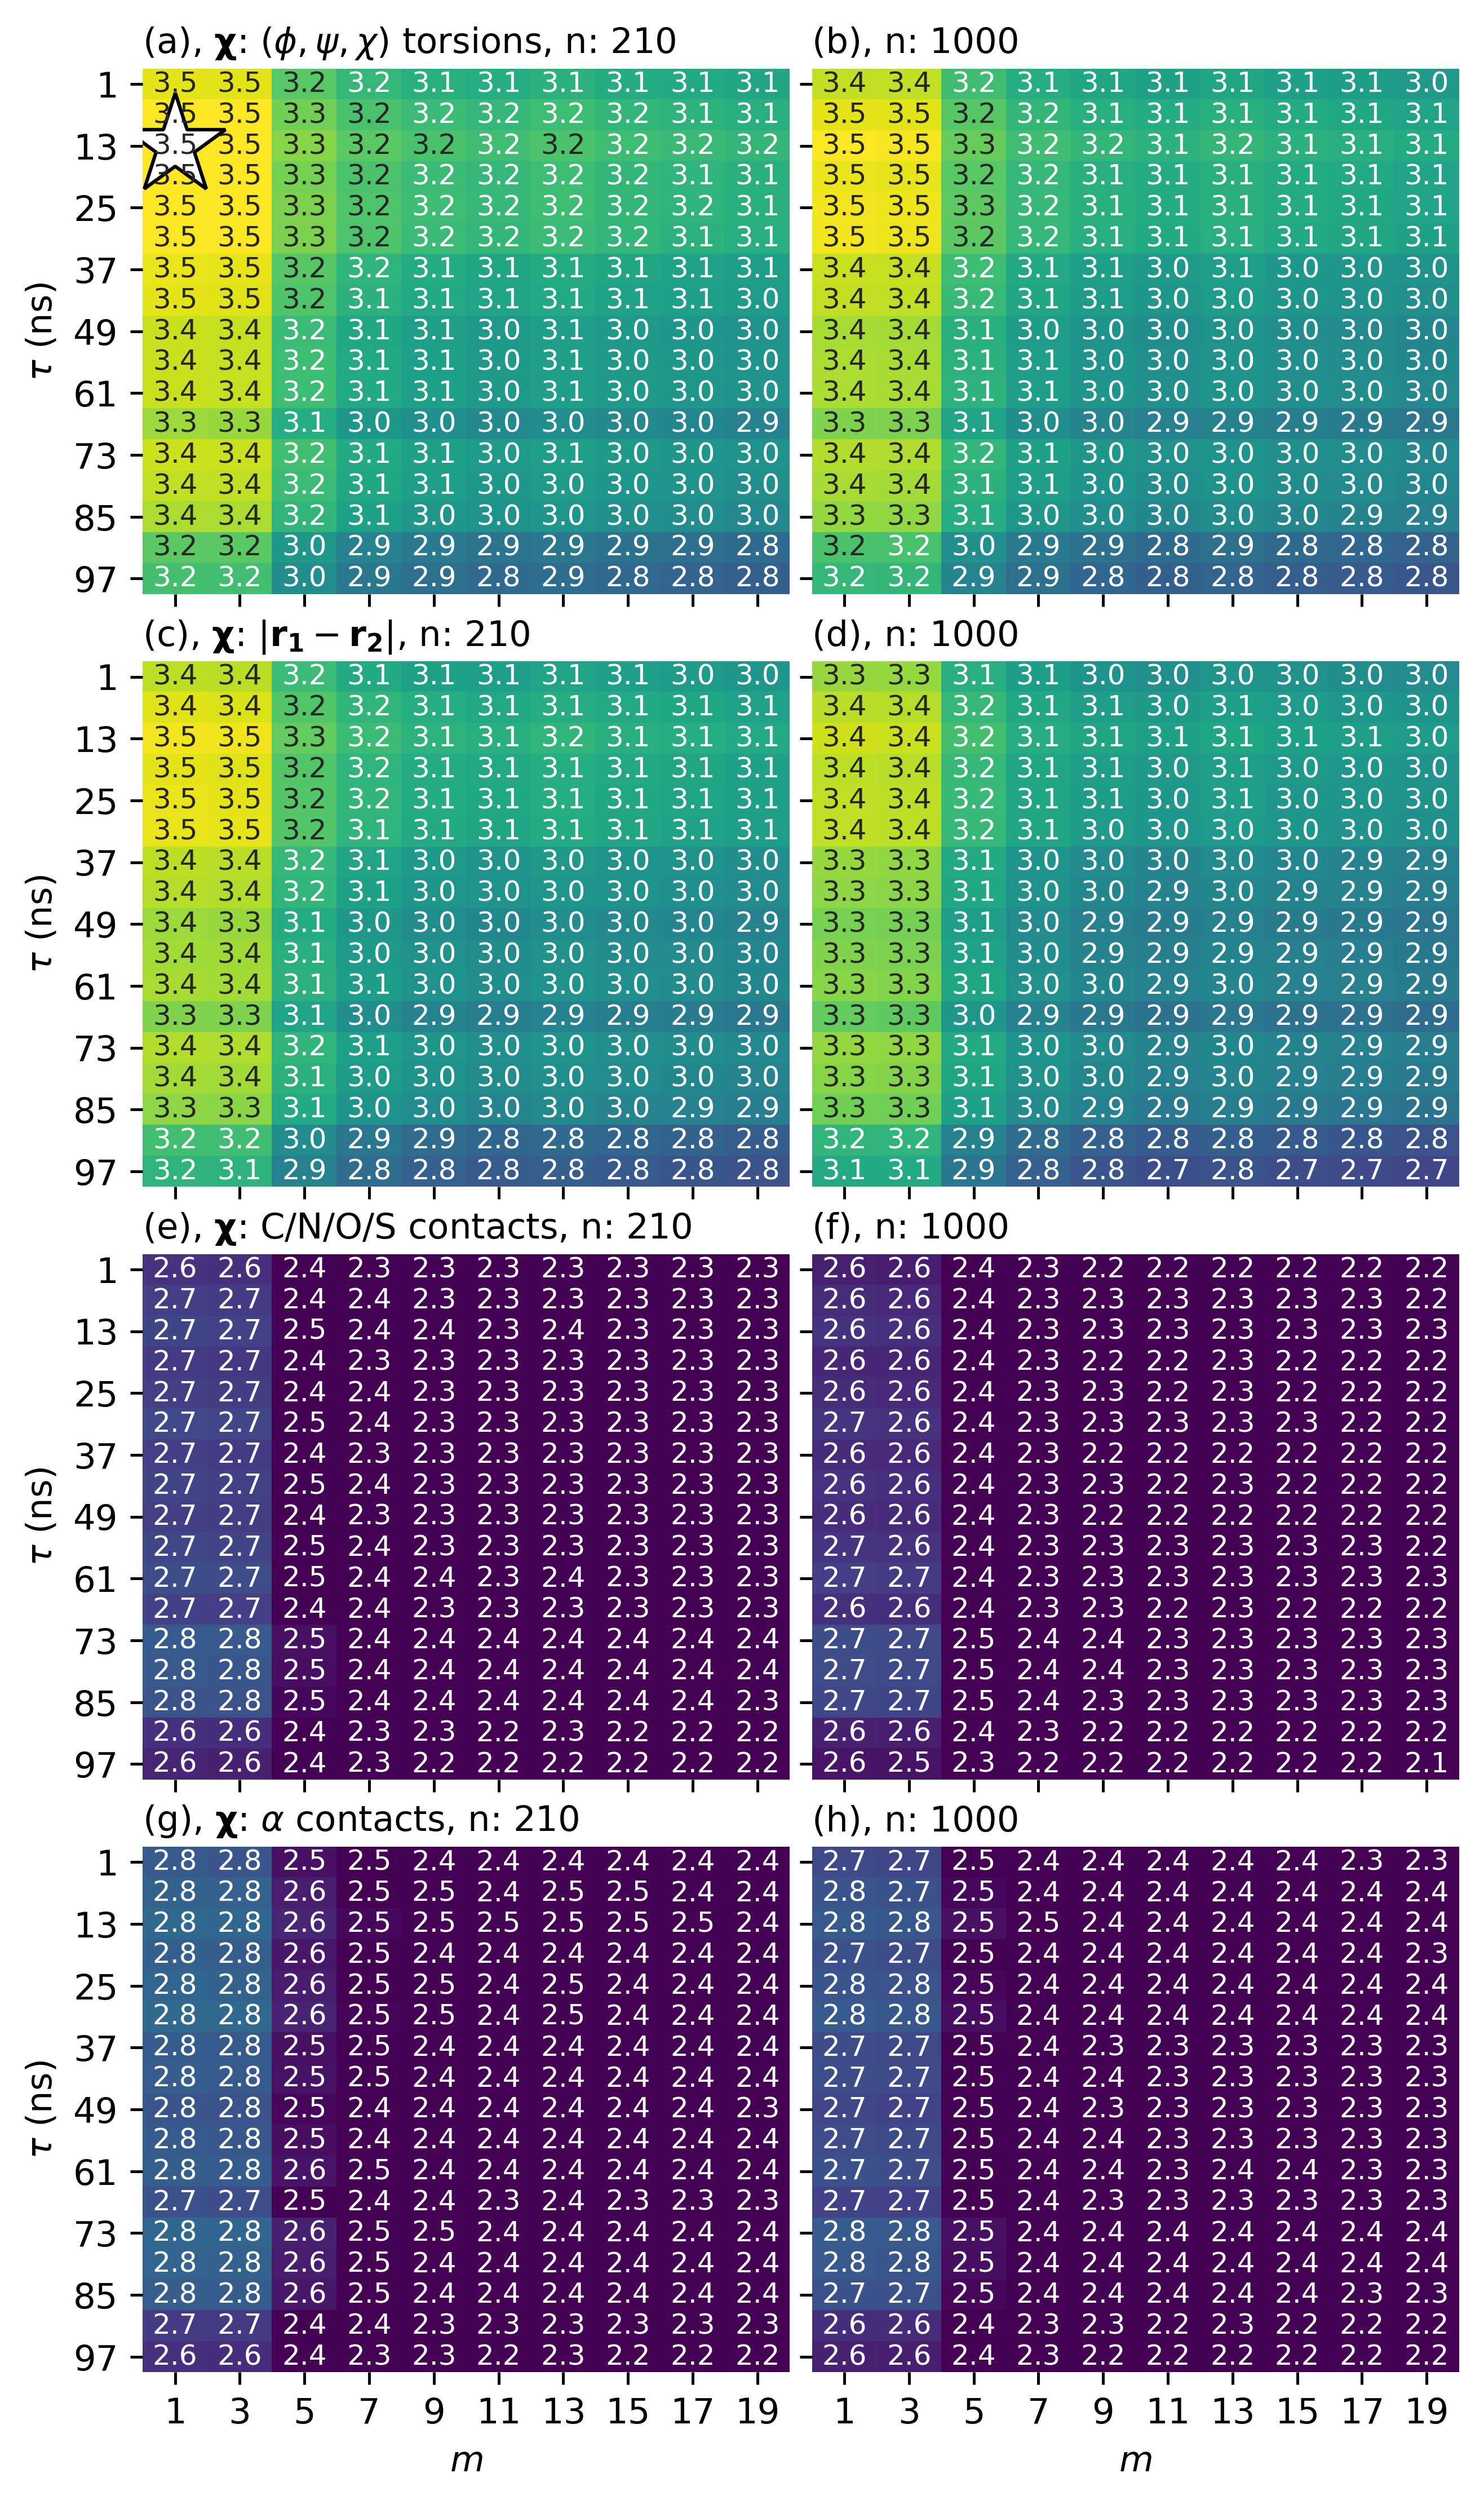
\includegraphics[width=0.7\textwidth]{chapters/msm_optimization/figures/aadh_response_surface_d.png}
    \label{fig:aadh_rsm}
\end{figure}

\begin{table}
    \centering
    \mycaption{Optimum MSM hyper-parameters for AADH pre- and post-Bayesian optimisation (BO). Each column represents a Bayesian optimisation experiment, seeded with $N_{seed}$ randomly sampled hyper-parameter trials. Five iterations of optimisation were run with $N_{seed}=100$ (labelled $\# 1, 2$ etc.) and a single iteration optimising the response surface using all the trial data ($N_{seed}=361$). Each row is a variable or outcome with values associated with the optimum value of $\mu$ before and after the BO.}
    \begin{tabular}{|ll|lllll|l|}
    \hline
    &$N_{seed}$ & 100 & & & & &361\\
    &\#&1&2&3&4&5&1\\
    \hline\hline
    $N_{total}$&Pre&100&100&100&100&100&361\\
    &Post&150&150&150&150&150&410\\
    \hline
    $\mu$&Pre&3.487&3.355&3.599&3.473&3.478&3.543\\
    &Post&3.500&3.558&3.545&3.581&3.569&3.558\\
    \hline
    $\sigma$&Pre&0.152&0.135&0.306&0.234&0.126&0.198\\
    &Post&0.202&0.117&0.101&0.084&0.072&0.091\\
    \hline
    $\chi$&Pre&$(\phi,\psi,\chi)$&$|\mathbf{r_{i}}-\mathbf{r_{j}}|$&$(\phi,\psi,\chi)$&$(\phi,\psi,\chi)$&$|\mathbf{r_{i}}-\mathbf{r_{j}}|$&$(\phi,\psi,\chi)$\\
    &Post&$(\phi,\psi,\chi)$&$(\phi,\psi,\chi)$&$(\phi,\psi,\chi)$&$(\phi,\psi,\chi)$&$(\phi,\psi,\chi)$&$(\phi,\psi,\chi)$\\
    \hline
    $\tau$&Pre&51.0&57.8&12.5&12.5&18.0&12.5\\
    &Post&1.0&4.0&3.0&1.0&1.0&10.0\\
    \hline
    $m$&Pre&1&3&1&1&1&1\\
    &Post&2&1&2&1&1&2\\
    \hline
    $n$&Pre&396&234&207&207&79&207\\
    &Post&10&180&10&230&540&310\\
    \hline
    \end{tabular}
    \label{tab:aadh_opt_results}
\end{table}

In order to test the convergence of the maximum of $f(\mathbf{x}; \mathcal{D}_{361})$, $50$ steps of Bayesian optimisation was performed. The values of the response and associated hyper-parameters pre- and post-optimisation (i.e. $f(\mathbf{x}; \mathcal{D}_{361})$ and $f(\mathbf{x}; \mathcal{D}_{410})$) are tabulated in table \ref{tab:aadh_opt_results}. The optimisation resulted in a small improvement in the response from $\mu=3.543 \pm 0.396 \rightarrow 3.558 \pm 0.182$ (a $\SI{0.4}{\percent}$ improvement) with no change in the optimum feature ($(\phi, \psi, \chi)$ dihedrals) and only small changes in the other hyper-parameters.  

In order to see whether this maximum could be reached with a fewer number of trials, five response surfaces fit on random subsets of the trial data with $100$ observations, $f^{i}(\mathbf{x};\mathcal{D}_{100}), i = 1 - 5$, were optimized with $50$ steps of Bayesian optimisation. The kernel and input warping for $f^{i}(\mathbf{x};\mathcal{D}_{100})$ were determined for each $i$ separately. The model selection metrics for each combination of kernel and input warping are tabulated in tables \ref{tab:aadh_rsm_metrics_iter_1} - \ref{tab:aadh_rsm_metrics_iter_5}. The results of the optimisation trials are shown in table \ref{tab:aadh_opt_results} and the incumbent trajectories are shown in are shown in figure \ref{fig:aadh_opt_traj_d}. Also shown in figure \ref{fig:aadh_opt_traj_d} are the maximum of the response surface $f(\mathbf{x};\mathcal{D}_{361})$ shown as orange lines, and the maximum of $f(\mathbf{x};\mathcal{D}_{410})$ shown as blue lines. 

\begin{figure}[p]
    \centering
    \mycaption{The Bayesian optimisation trajectories for AADH. Each column shows the trajectories of the incumbent $\mu\pm 2\sigma$ (panels (a) - (e)), and the accompanying value of: $\chi$ (panels (f) - (j)), $m$ (panels (k) - (o)), $\tau$ (panels (p) - (t)) and $n$ (panels (u) - (y)). The location of the final value of the trajectory is highlighted with a black star. For reference the corresponding values determined from the response surface using all the hyper-parameter trials are shown as solid horizontal lines: the response surface before optimisation are shown in orange and after Bayesian optimisation in blue.}
    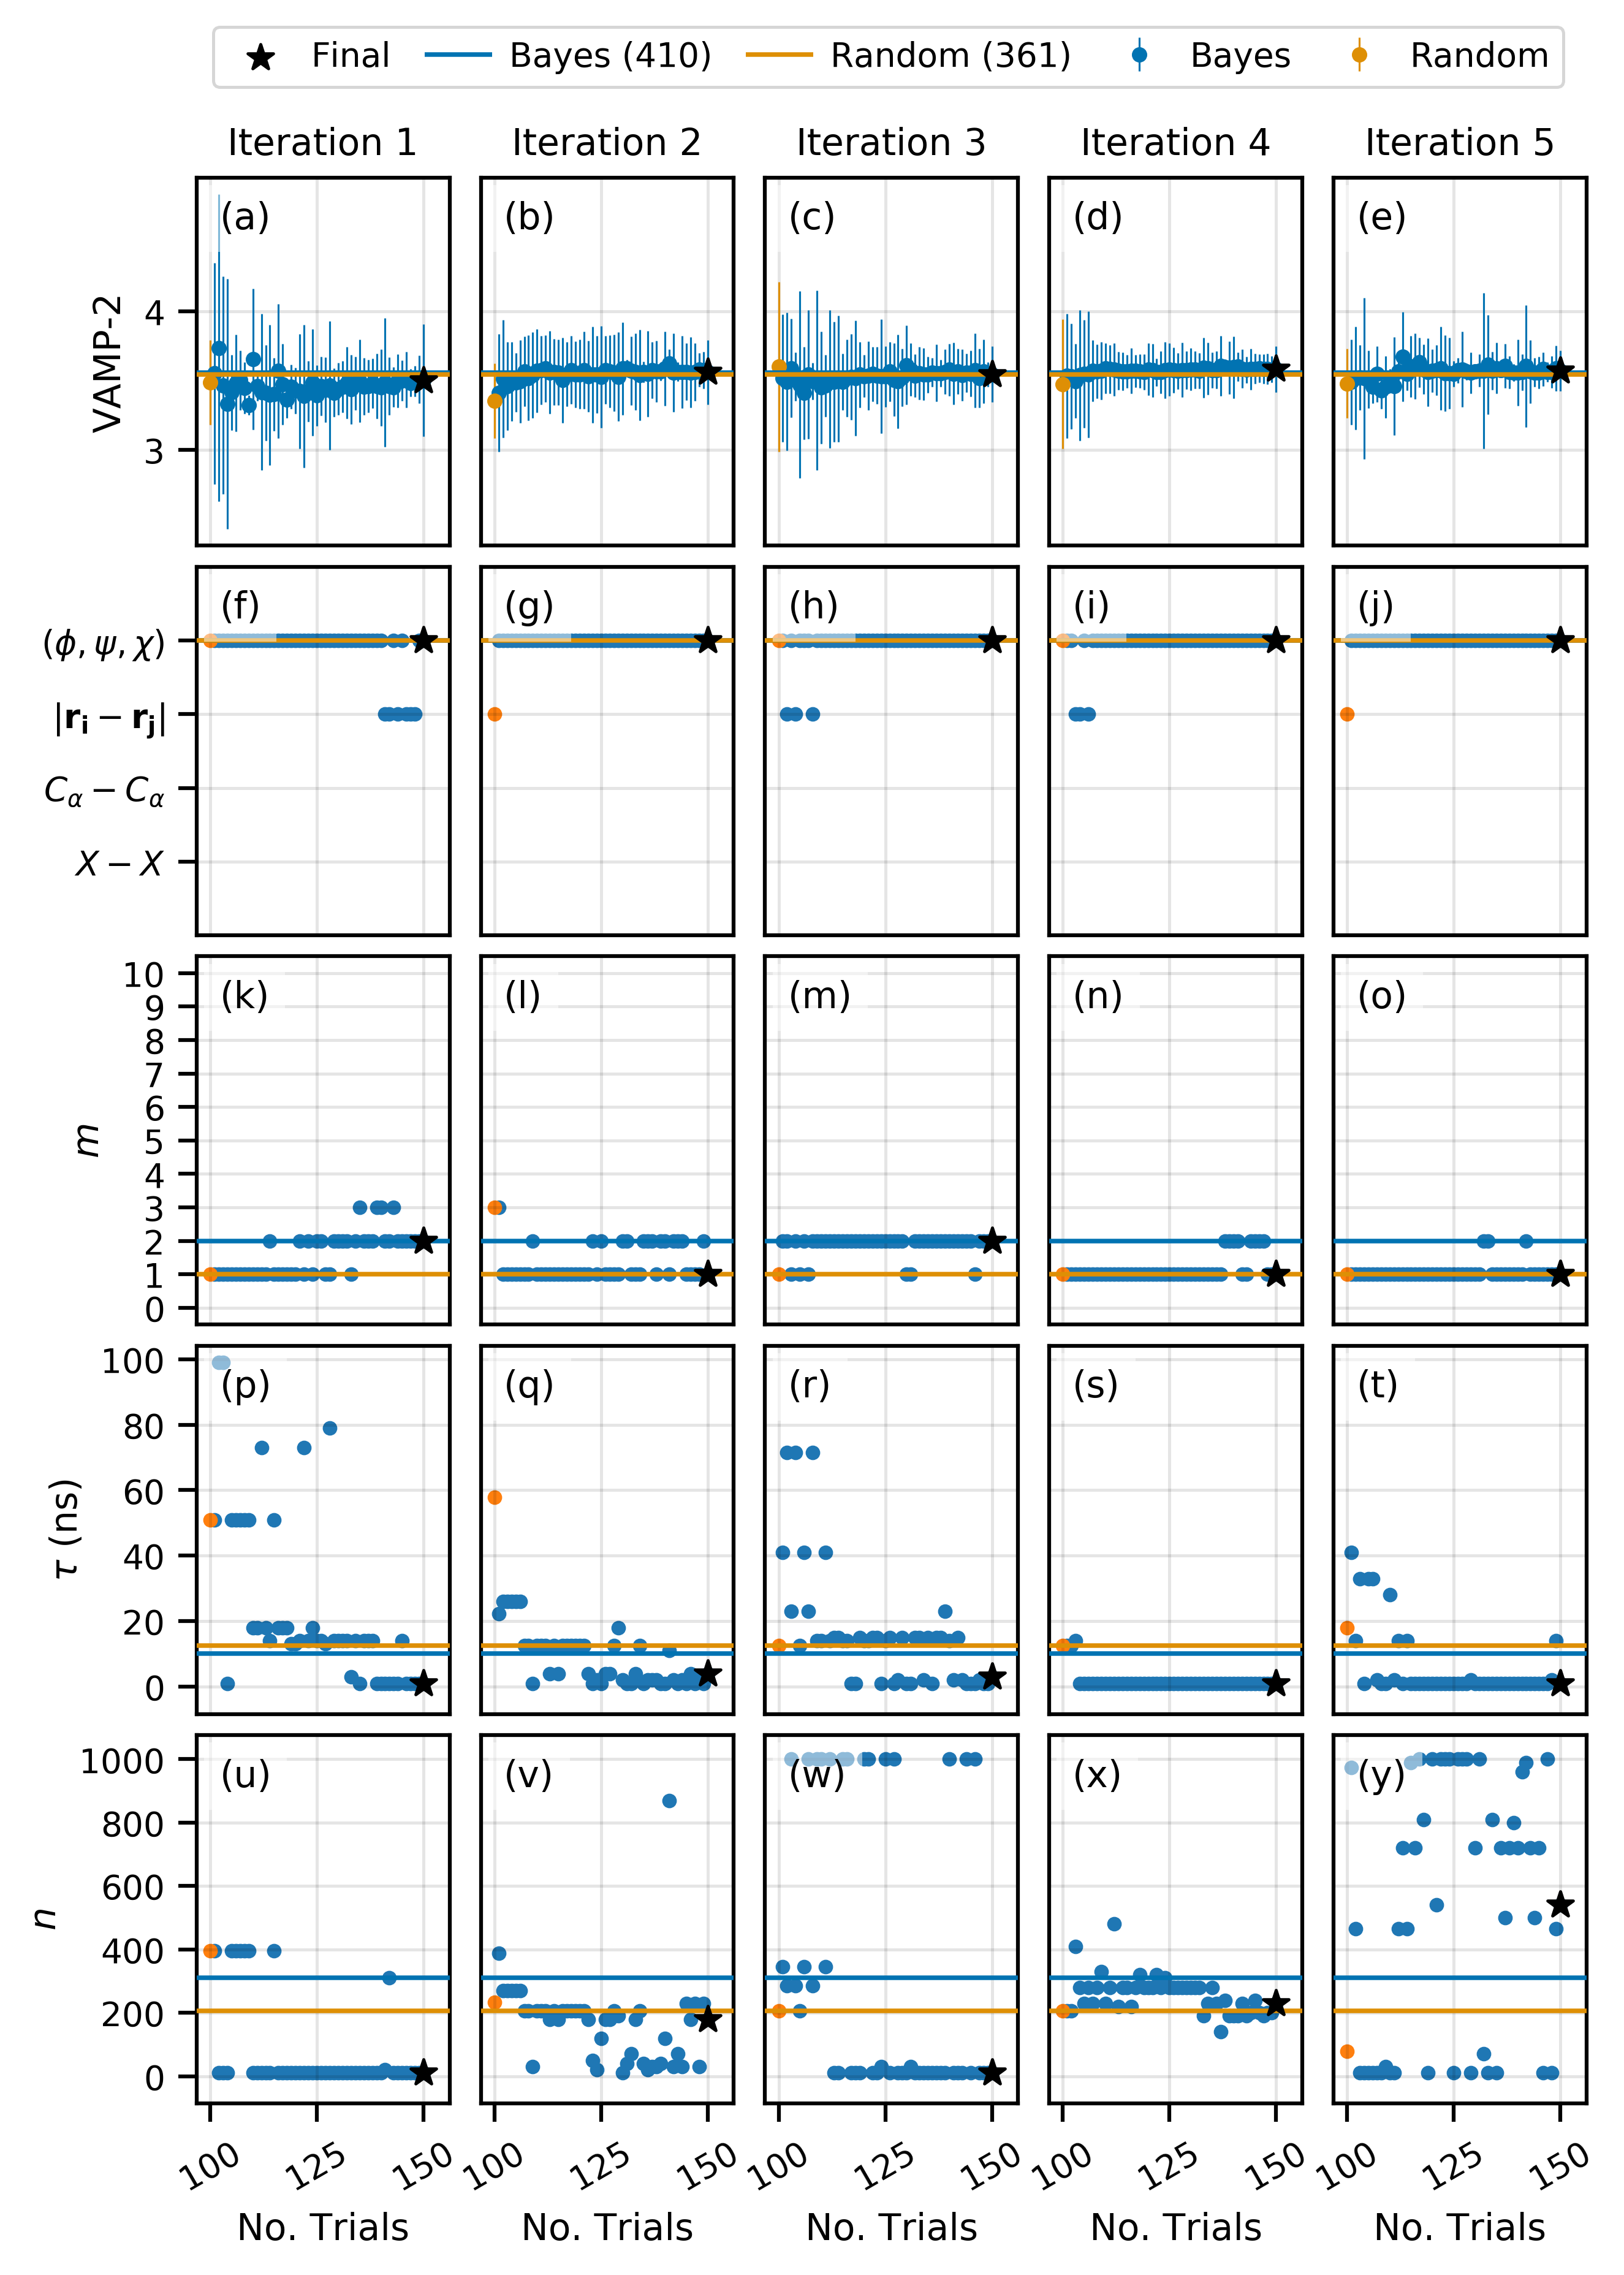
\includegraphics[width=0.8\textwidth]{chapters/msm_optimization/figures/aadh_opt_traj_act_s_d.png}
    
    \label{fig:aadh_opt_traj_d}
\end{figure}

 It is clear from  table \ref{tab:aadh_opt_results} that after Bayesian optimisation each subset had maxima indistinguishable from the maxima of $f(\mathbf{x};\mathcal{D}_{461})$: each had the same optimal feature ($(\phi, \psi, \chi)$ dihedrals), slightly smaller values of $\tau$ ($1 - \SI{4}{\nano\second}$ cf. $\SI{10}{\nano\second}$), similar values of $m$ ($1 - 2$ cf. $2$) but with a range of different values of $n$ ($10 - 540$ cf. $310$). The extent to which these differences to make a difference the final MSM and its interpretation will be discussed in section \ref{subsubsec:sensitivity_analysis} in the context of several sensitivity analyses. 
 
It is also clear that Bayesian optimisation only had a small effect on the value of the incumbent and on the optimum hyper-parameters.  The value of incumbent throughout the procedure (figure \ref{fig:aadh_opt_traj_d} panels (a) - (e)) remain relatively flat. The largest increase came from iteration $4$, with $\Delta \mu 0.108$ and there was even a slight decrease in iteration $3$ with $\Delta \mu = -0.054$. The optimisation procedure also had negligible effects on the value of $\chi$, $m$ and $n$. It did however explore large values of  $\tau$ before settling on its final optimum value in most of the iterations.

The maxima and optimum hyper-parameters of the optimized response surfaces $f^{i}(\mathbf{x};\mathcal{D}_{150})$ are almost indistinguishable from $f(\mathbf{x};\mathcal{D}_{461})$. However the optimisation procedure did not strongly affect the optima of $f^{i}(\mathbf{x};\mathcal{D}_{100})$ compared to $f^{i}(\mathbf{x};\mathcal{D}_{150})$. This suggests that the Bayesian optimisation procedure could be seeded with much fewer trials if a GP model of the response surface could be estimated reliably. 

\subsubsection{Sensitivity analysis}\label{subsubsec:sensitivity_analysis}

\begin{figure}
    \centering
    \mycaption{Implied timescales of the MSM of AADH with optimized hyper-parameters, estimated using MCMC with 500 posterior draws. Panel (a) shows the implied timescales for $0.1 < \tau(\mathrm{MSM})< \SI{5}{\nano\second}$ and panel (b) for $1 < \tau(\mathrm{MSM}) <\SI{50}{\nano\second}$. The solid lines are the mean of the posteriors, the coloured shaded areas are the  $\SI{95}{\percent}$ credible intervals. The grey shaded area is the region for which the implied timescales are smaller than $\tau(\mathrm{MSM})$.}\label{fig:aadh_its}
    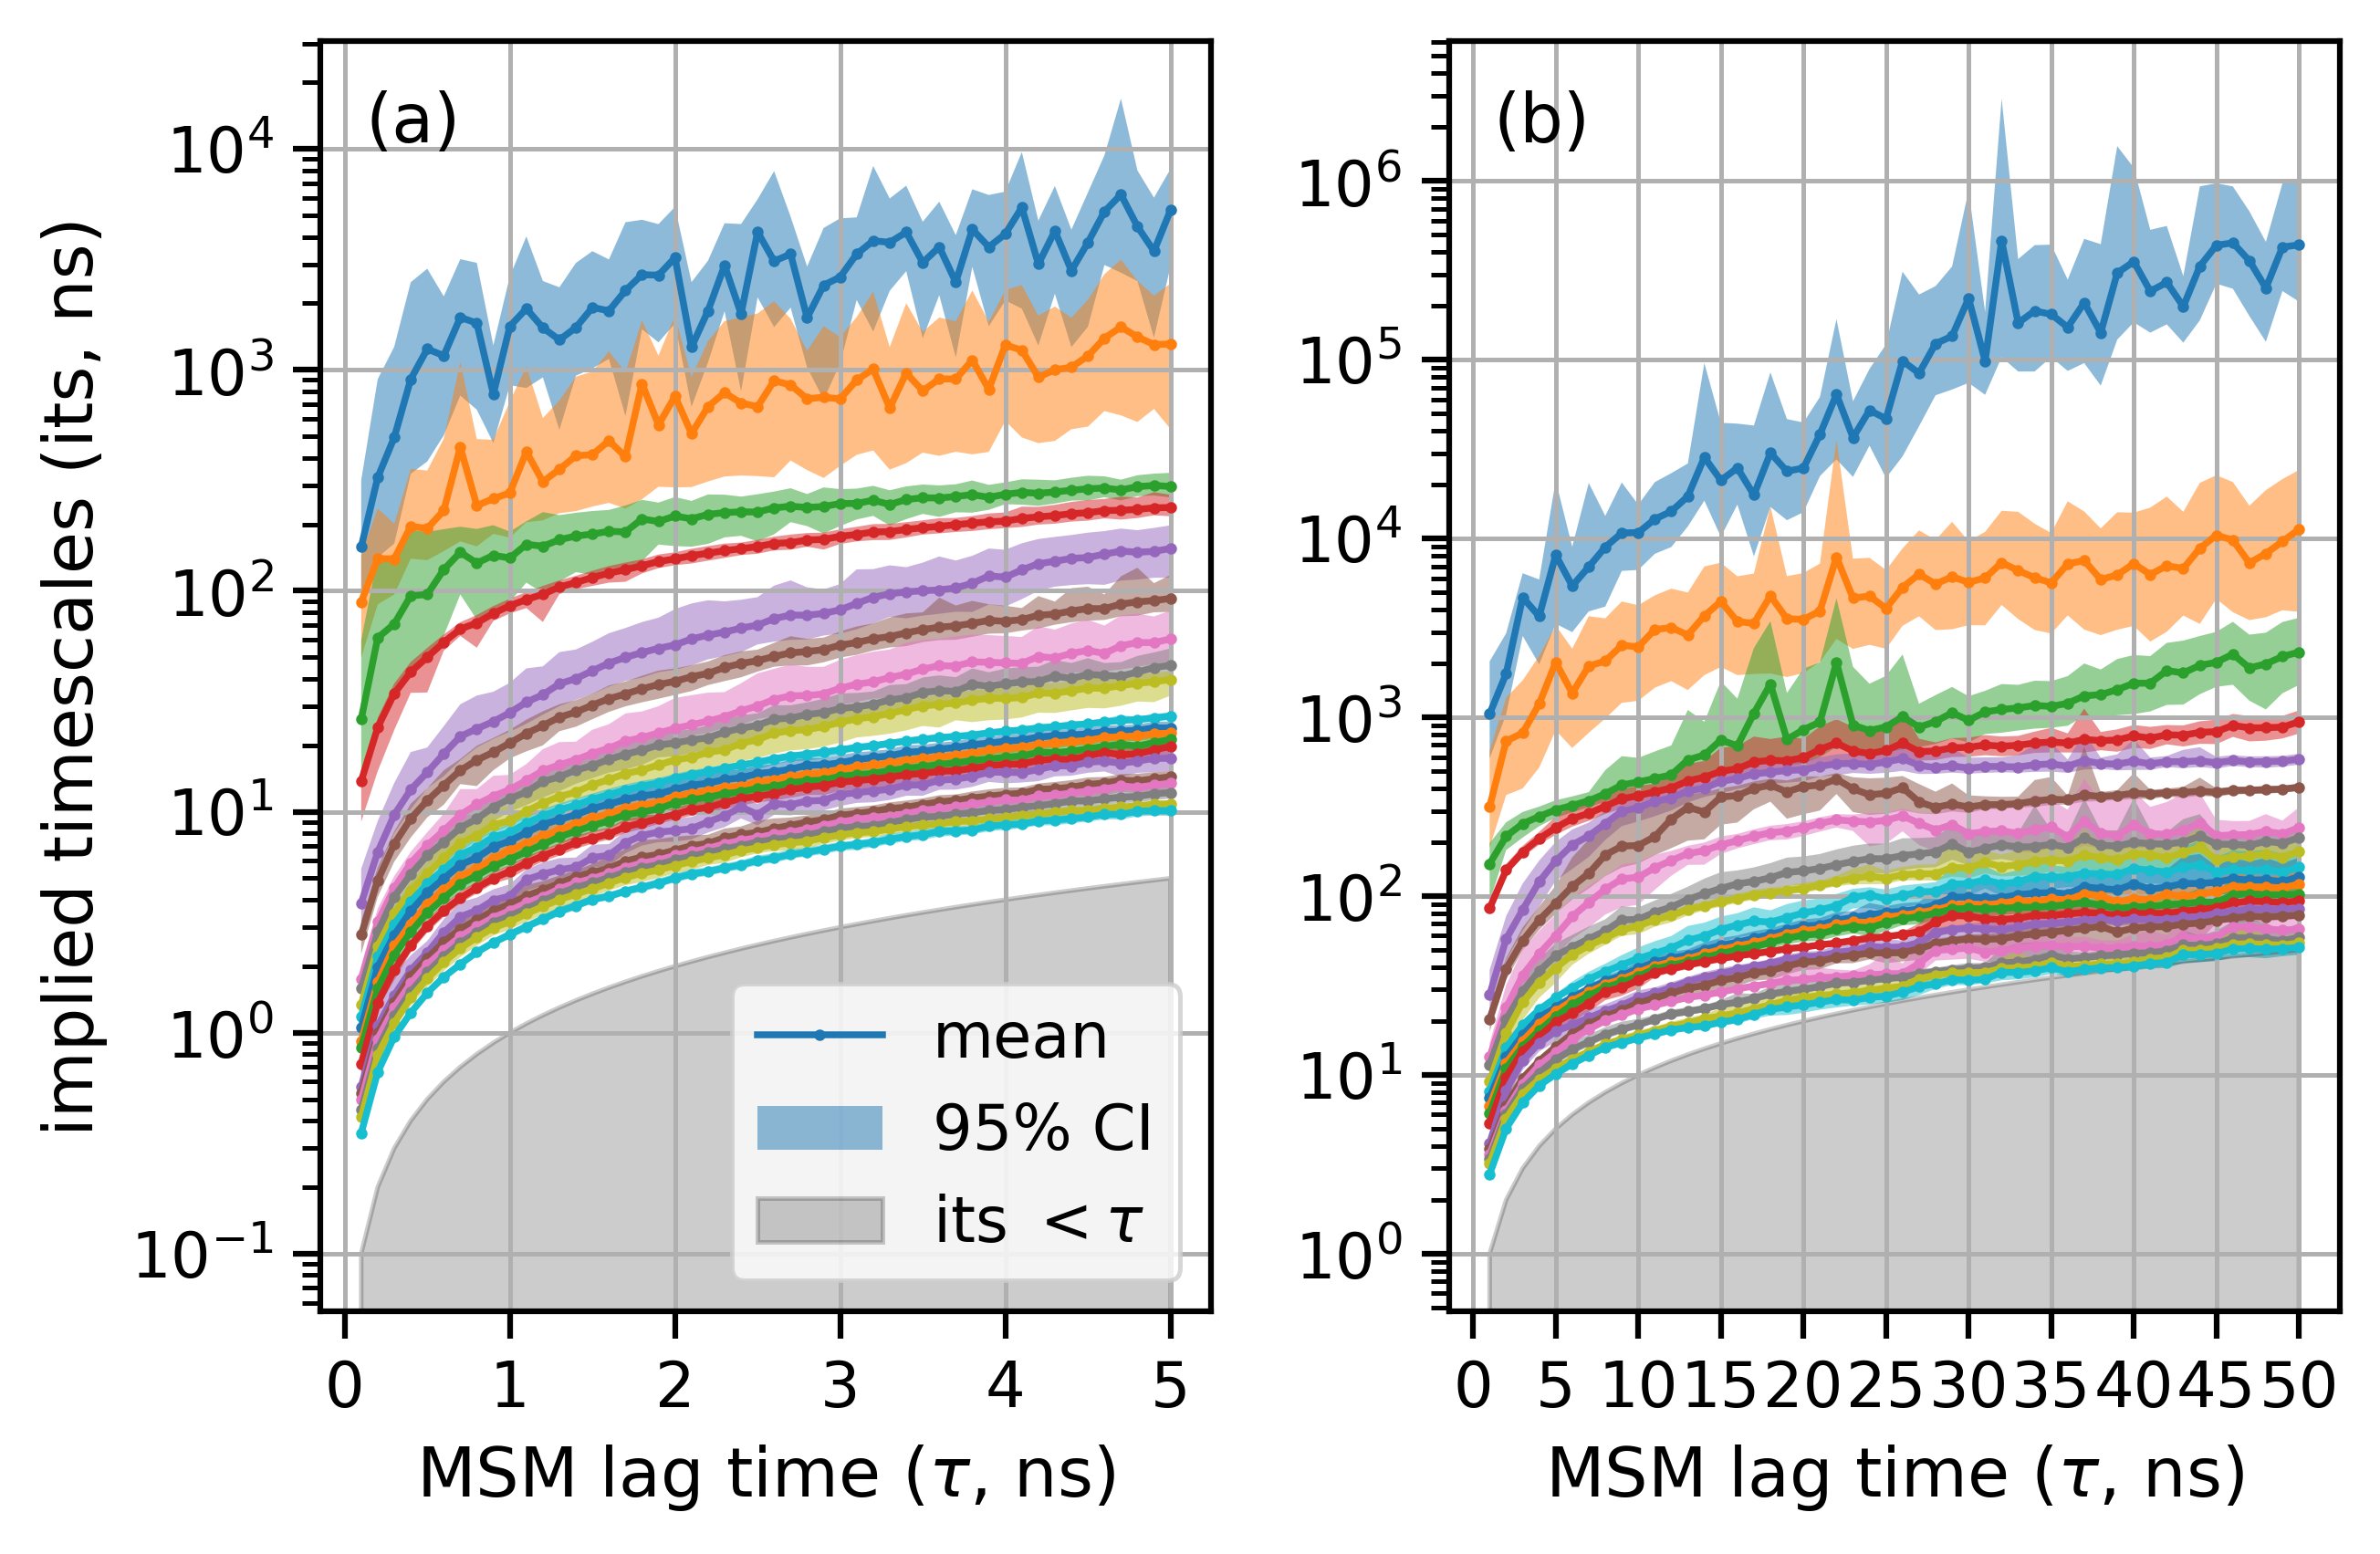
\includegraphics[width=0.9\linewidth]{chapters/msm_optimization/figures/aadh_implied_timescales.png}
\end{figure}

So far the response surface for AADH has been modelled and optimised with a combination of random hyper-parameter sampling and Bayesian optimisation under two assumptions about the model specification: that $\tau(\mathrm{MSM}) = \SI{2}{\nano\second}$ and $k=4$, the number of eigenvalues in the VAMP-2 score, are reasonable assumptions about the lag time and number of slow relaxation processes. As these were established on the basis of the reference MSM it is important to to test these assumptions are still reasonable with the final optimized MSM. 

To test the suitability of $\tau(\mathrm{MSM})$ the eigenvalue spectra of a series of MSMs fit with the optimum hyper-parameters (with $N_{total}=410$, table \ref{tab:aadh_opt_results}) but different lag times are shown in figure \ref{fig:aadh_its}. Panel (a) shows shows lags of  $\SI{0.1}{\nano\second} < \tau(\mathrm{MSM}) < \SI{5}{\nano\second}$ which clearly shows there is a slight increase in the top two implied timescales ($t_{2}$ and $t_{3}$\footnote{I'm using the convention that $t_{1} = \infty$, whose associated eigenvector is the stationary distribution}), suggesting that $\tau^{MSM}$ may be too small. Looking at the implied timescales on a longer timescale $1 < \tau^{MSM} < \SI{50}{\nano\second}$ (panel (b)) shows that there is a small plateau in $t_{2}$ and $t_{3}$  around  $\SIrange{15}{20}{\nano\second}$. It is therefore not possible on this evidence alone to say definitively whether $\tau(\mathrm{MSM})$ should be $2$ or $\SI{20}{\nano\second}$ or whether it makes a difference to non-quantitative aspects of the final model.  

At $\tau = \SI{2}{\nano\second}$ there is no clear separation of timescales between the first four relaxation processes (taking into account the uncertainty in $t_{2}$ and $t_{3}$), however there is a gap between $t_{5}$ and $t_{6}$ suggesting $k=5$ would be more appropriate. This means the fourth relaxation process ($t_{5}$, shown in red in figure \ref{fig:aadh_its}) has not been factored into the response. In principle this means that there may be different hyper-parameters which maximize $\operatorname{VAMP}-2(k=5)$,  given the similarity in $t_{4}$ and $t_{5}$ this may not be very plausible or significant if true. At $\tau = \SI{20}{\nano\second}$ there is a clear separation between $t_{2}$ and $t_{3}$ suggesting $k=2$ is appropriate. In this case we have included potentially too many fast processes. While changing the value of $k$ will certainly change the value of the optimal hyper-parameters, given the mixed evidence in the eigenvalue spectrum there is no reason to reject this optimized MSM. The associated question of how many metastable states and dominant relaxation processes actually matter for explaining the observed data will be investigated further in chapter \ref{chap:hmm}. 

Knowledge of the response surface and of the eigenvalue spectrum suggests sensitivity analyses to understand the validity and robustness of the optimum MSM.  The goal of sensitivity analyses is to have faith that reasonable changes in model choices and hyper-parameters do not materially affect inferences from the model. Typically we are concerned with inferring relaxation timescales ($t_{i}$), the character of the relaxation process ($\Psi_{i}$) and the lumping of the microstates into metastable states. The VAMP-2 score has served as a proxy for the quality of the inferences required from the model but this is not sufficient  for a number of reasons.  First, as discussed above it will be sensitive to both the MSM lag time and the number of eigenfunctions used in the definition. Second, as figure \ref{fig:ala1_evcompare} has demonstrated, VAMP-2 is not sensitive to the discretisation error. This is also evident in the fact that in both iteration $1$ and $3$ (table \ref{tab:aadh_opt_results}) the optimal value of $n=10$ with only a very small difference in response at these values $\mu = 3.500$ and   $\mu=3.545$ cf. $\mu=3.558$). Third, the phenomenon of the Rashomon effect \cite{breiman2001} in statistical modelling, where  multiple \emph{different} statistical models result in the performance metric, could be at play here.

The standard validation check of MSMs, the Chapman-Kolmogorov test (equation \ref{eqn:ck_test}), relies on coarse graining transition matrix, which will be discussed in detail in chapter \ref{chap:hmm}. The current discussion will center on the eigenvalue spectrum and qualitative aspects of the free energy surface and eigenfunctions. For the optimal MSM, these are all shown in figure \ref{fig:aadh_msm_best}: panels (a) - (c) show the normalised eigenvectors of the first three relaxation processes ($\Psi_{2} - \Psi_{3}$) in the space of the first two TICA components. A coarse grained color map has been applied to make the sign structure, rather than the absolute value of eigenvector, more apparent: $|\Psi_{2}| < 1e^{-2}$ are coloured white, $\Psi_{2}> 0$ red,  and $\Psi_{2} < 0$ blue. Panel (d) shows the implied timescales for the first $10$ relaxation processes (coloured according to whether they were included in the $\operatorname{VAMP-2}$ score), and panel (e) shows the free energy surface in the space of the first two TICA components. 

\begin{figure}
    \centering
    \mycaption{The final, optimised response surface of AADH fit using the $361$ randomly sampled hyper-parameter trials and the $50$ trials selected in the Bayesian optimisation procedure. For each feature a single heat map are shown for $n=310$, with $\tau$ on the vertical axis and $m$ on the horizontal axis. All values of $m$ in the range $1\le m \le 10$ are shown. The white star denotes the approximate location of the maximum of the surface, the true maximum occurs at $\tau=\SI{10}{\nano\second}, m=2, n=310$. The value of the response surface denoted by the color (lighter implied higher values) and with the text annotations. }
    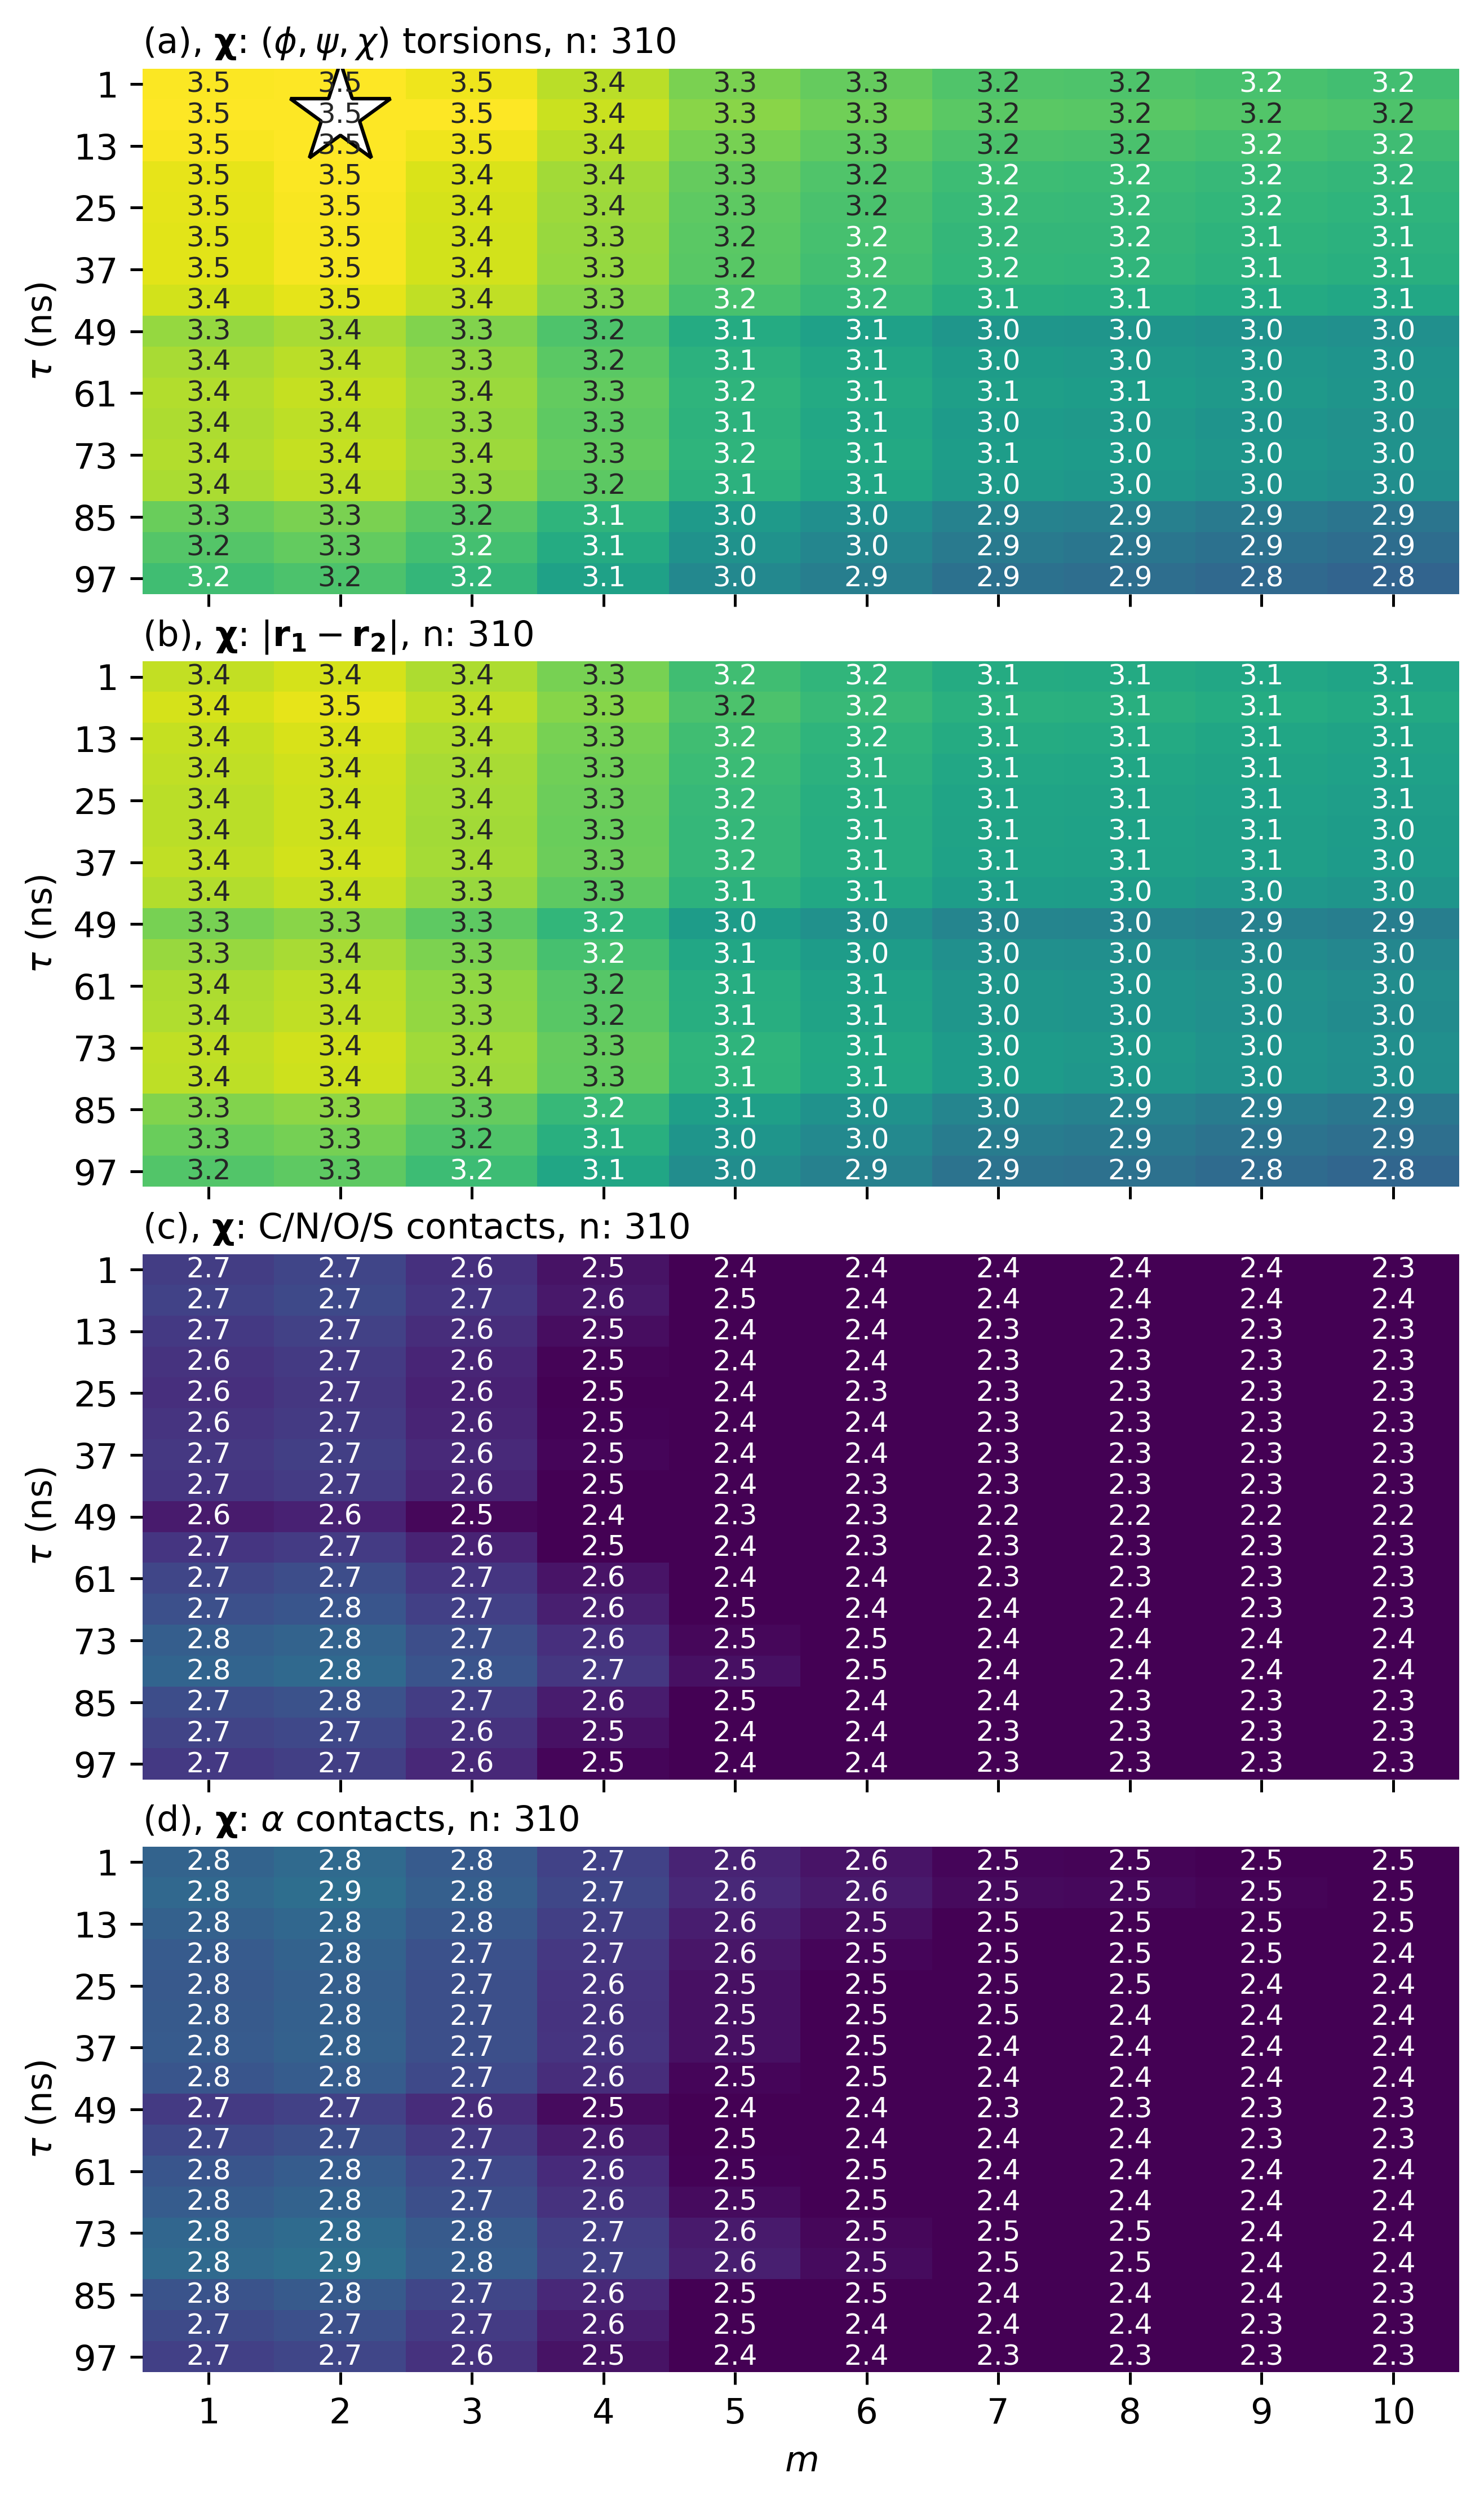
\includegraphics[width=0.6\textwidth]{chapters/msm_optimization/figures/aadh_response_surface_d_opt.png.png}
    \label{fig:aadh_rsm_opt}
\end{figure}


\begin{figure}
    \centering
    \mycaption{[TM: label axes] MSM of AADH with optimum hyper-parameters: $\chi= (\phi, \psi, \chi)$ torsions, $\tau=\SI{10}{\nano\second}$, $m=2$ and $n=310$. Panels (a), (b) and (c) show the non-trivial eigenvectors used in the VAMP-2 score, the horizontal and vertical axes are the first two TICA components. Panel (d) are the first ten implied timescales, colored according to whether they were used in the VAMP-2 score. The error bars are the $\SI{95}{\percent}$ credible intervals.  Panel (e) is the free energy with the same axes as panels (a) - (c). The MSM was estimated using MCMC with 1000 samples of the posterior.}
    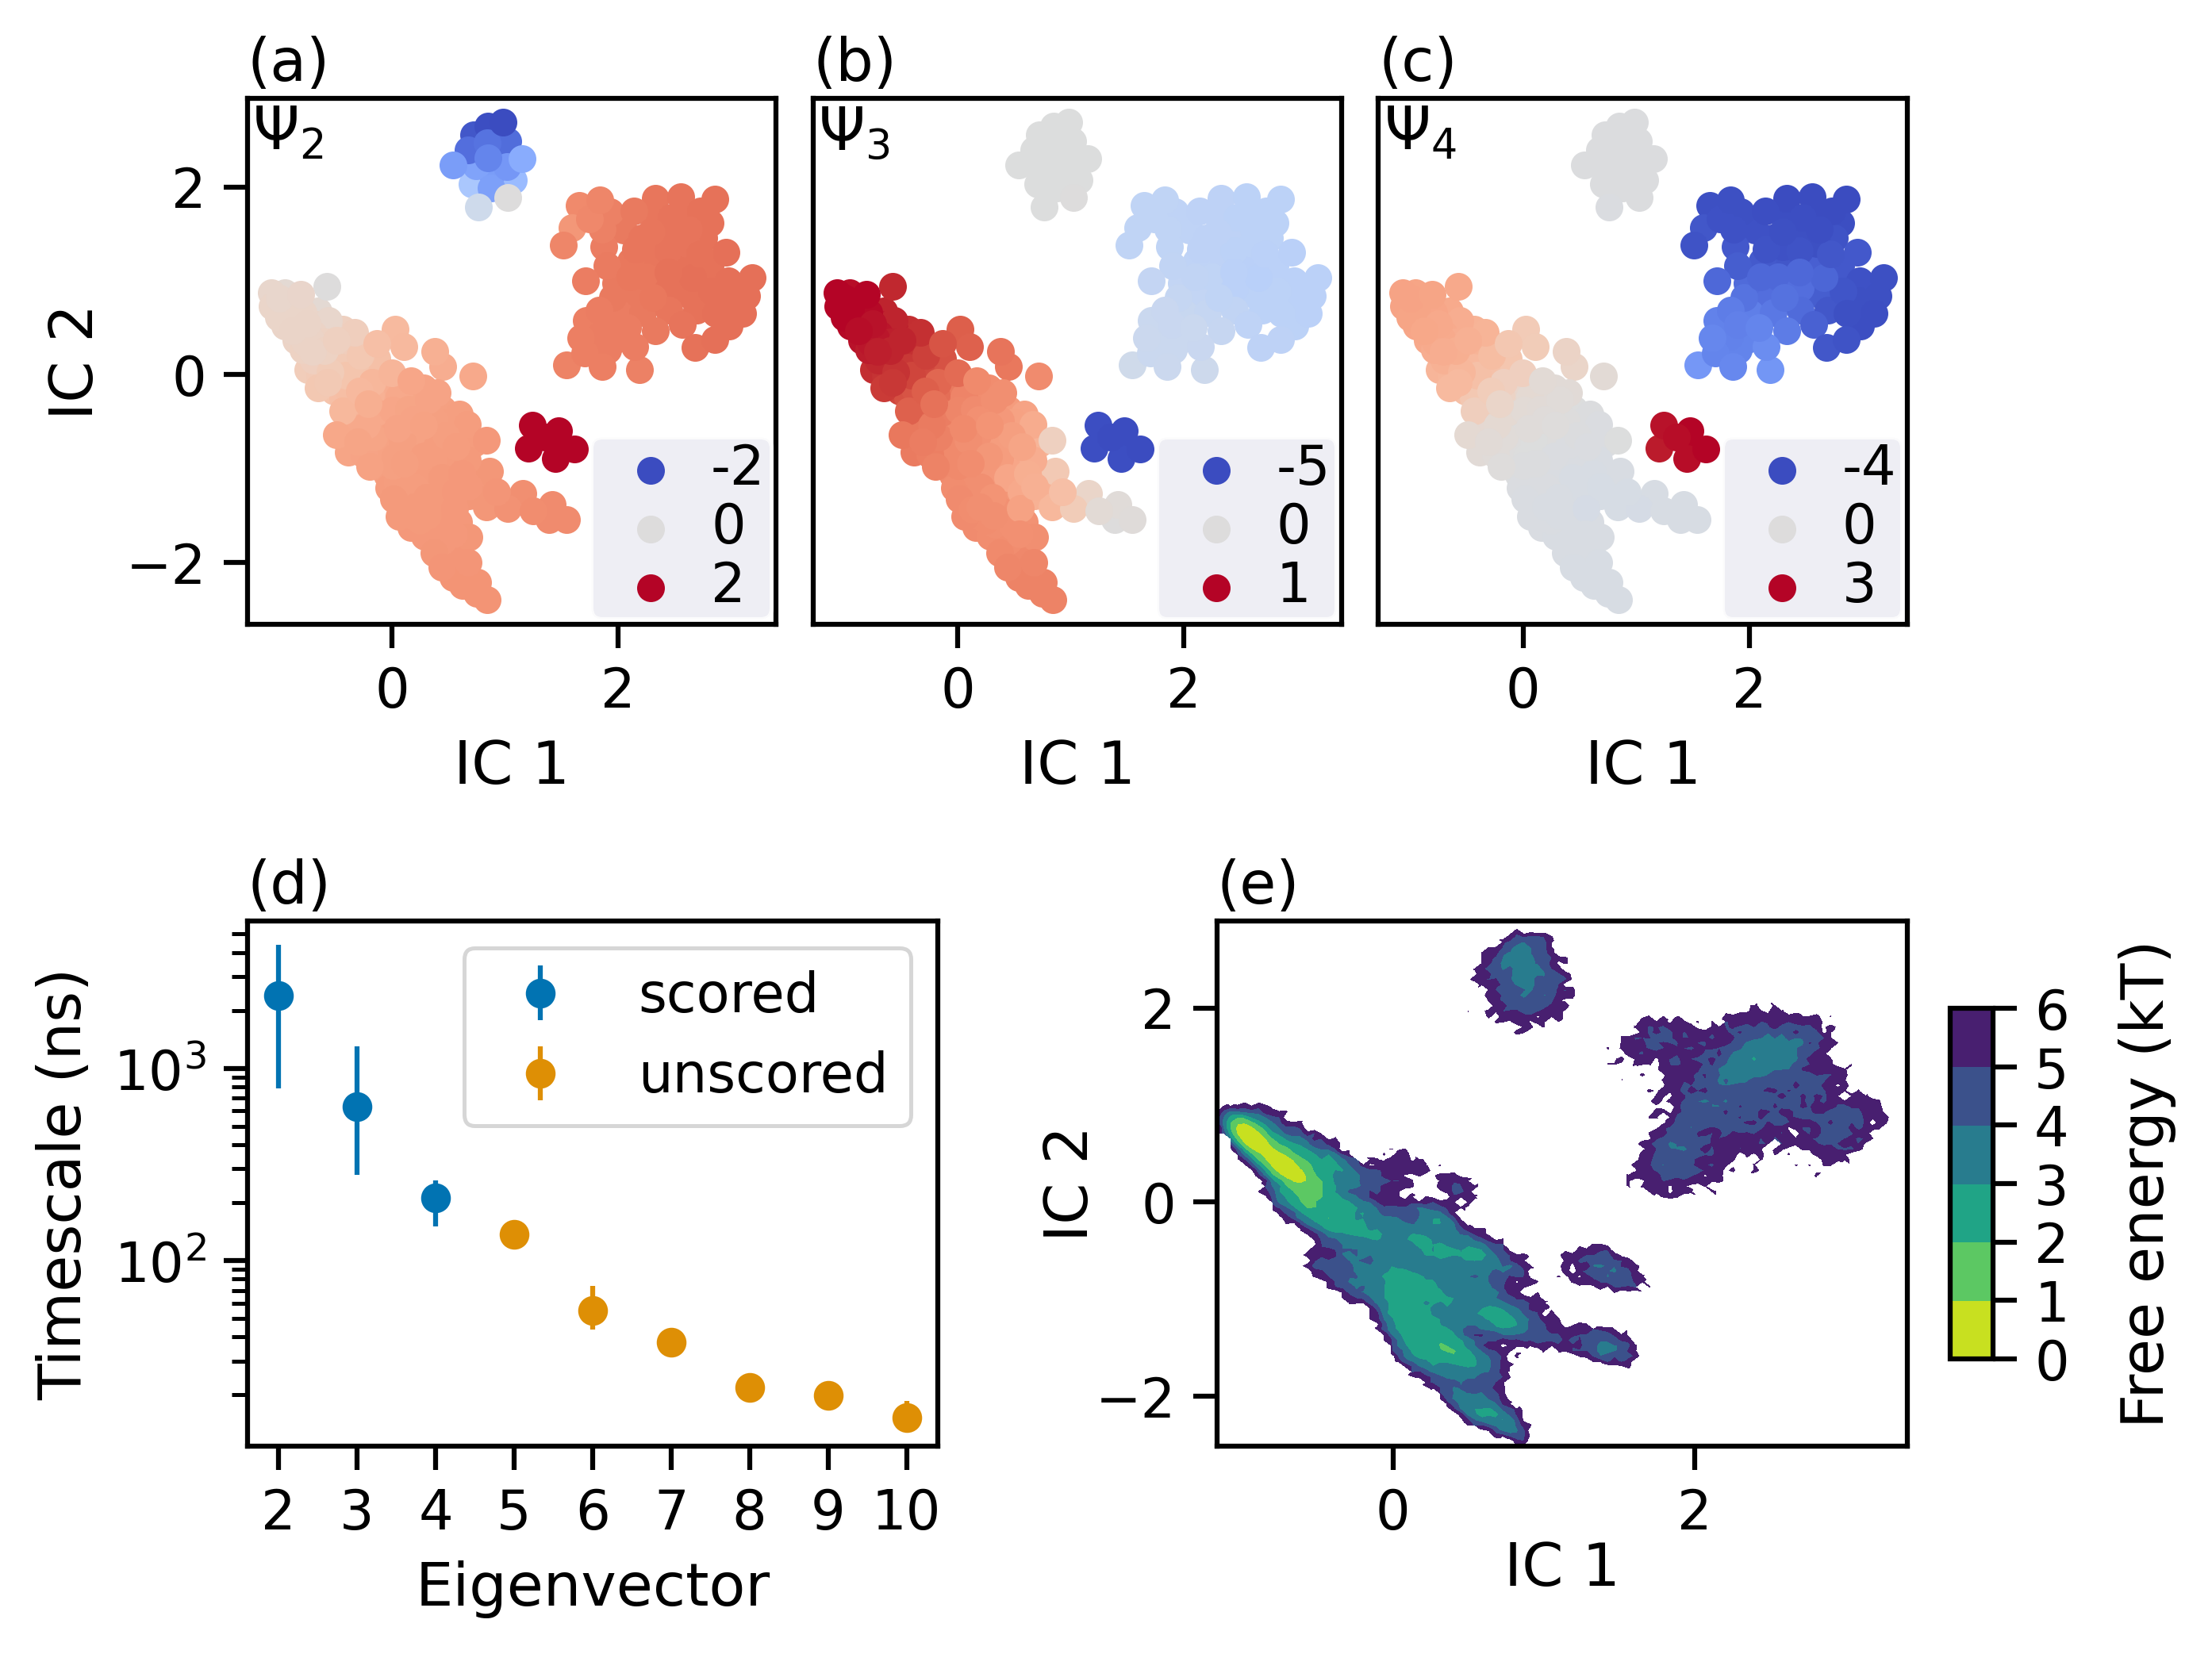
\includegraphics[width=0.7\textwidth]{chapters/msm_optimization/figures/aadh_msm_best.png}
    \label{fig:aadh_msm_best}
\end{figure}

\begin{figure}
    \centering
    \mycaption{Sensitivity 1: MSM of AADH with the same hyper-parameters as the base case  but with $\tau(\mathrm{MSM})=\SI{20}{\nano\second}$. See caption of figure \ref{fig:aadh_msm_best} for details. }
    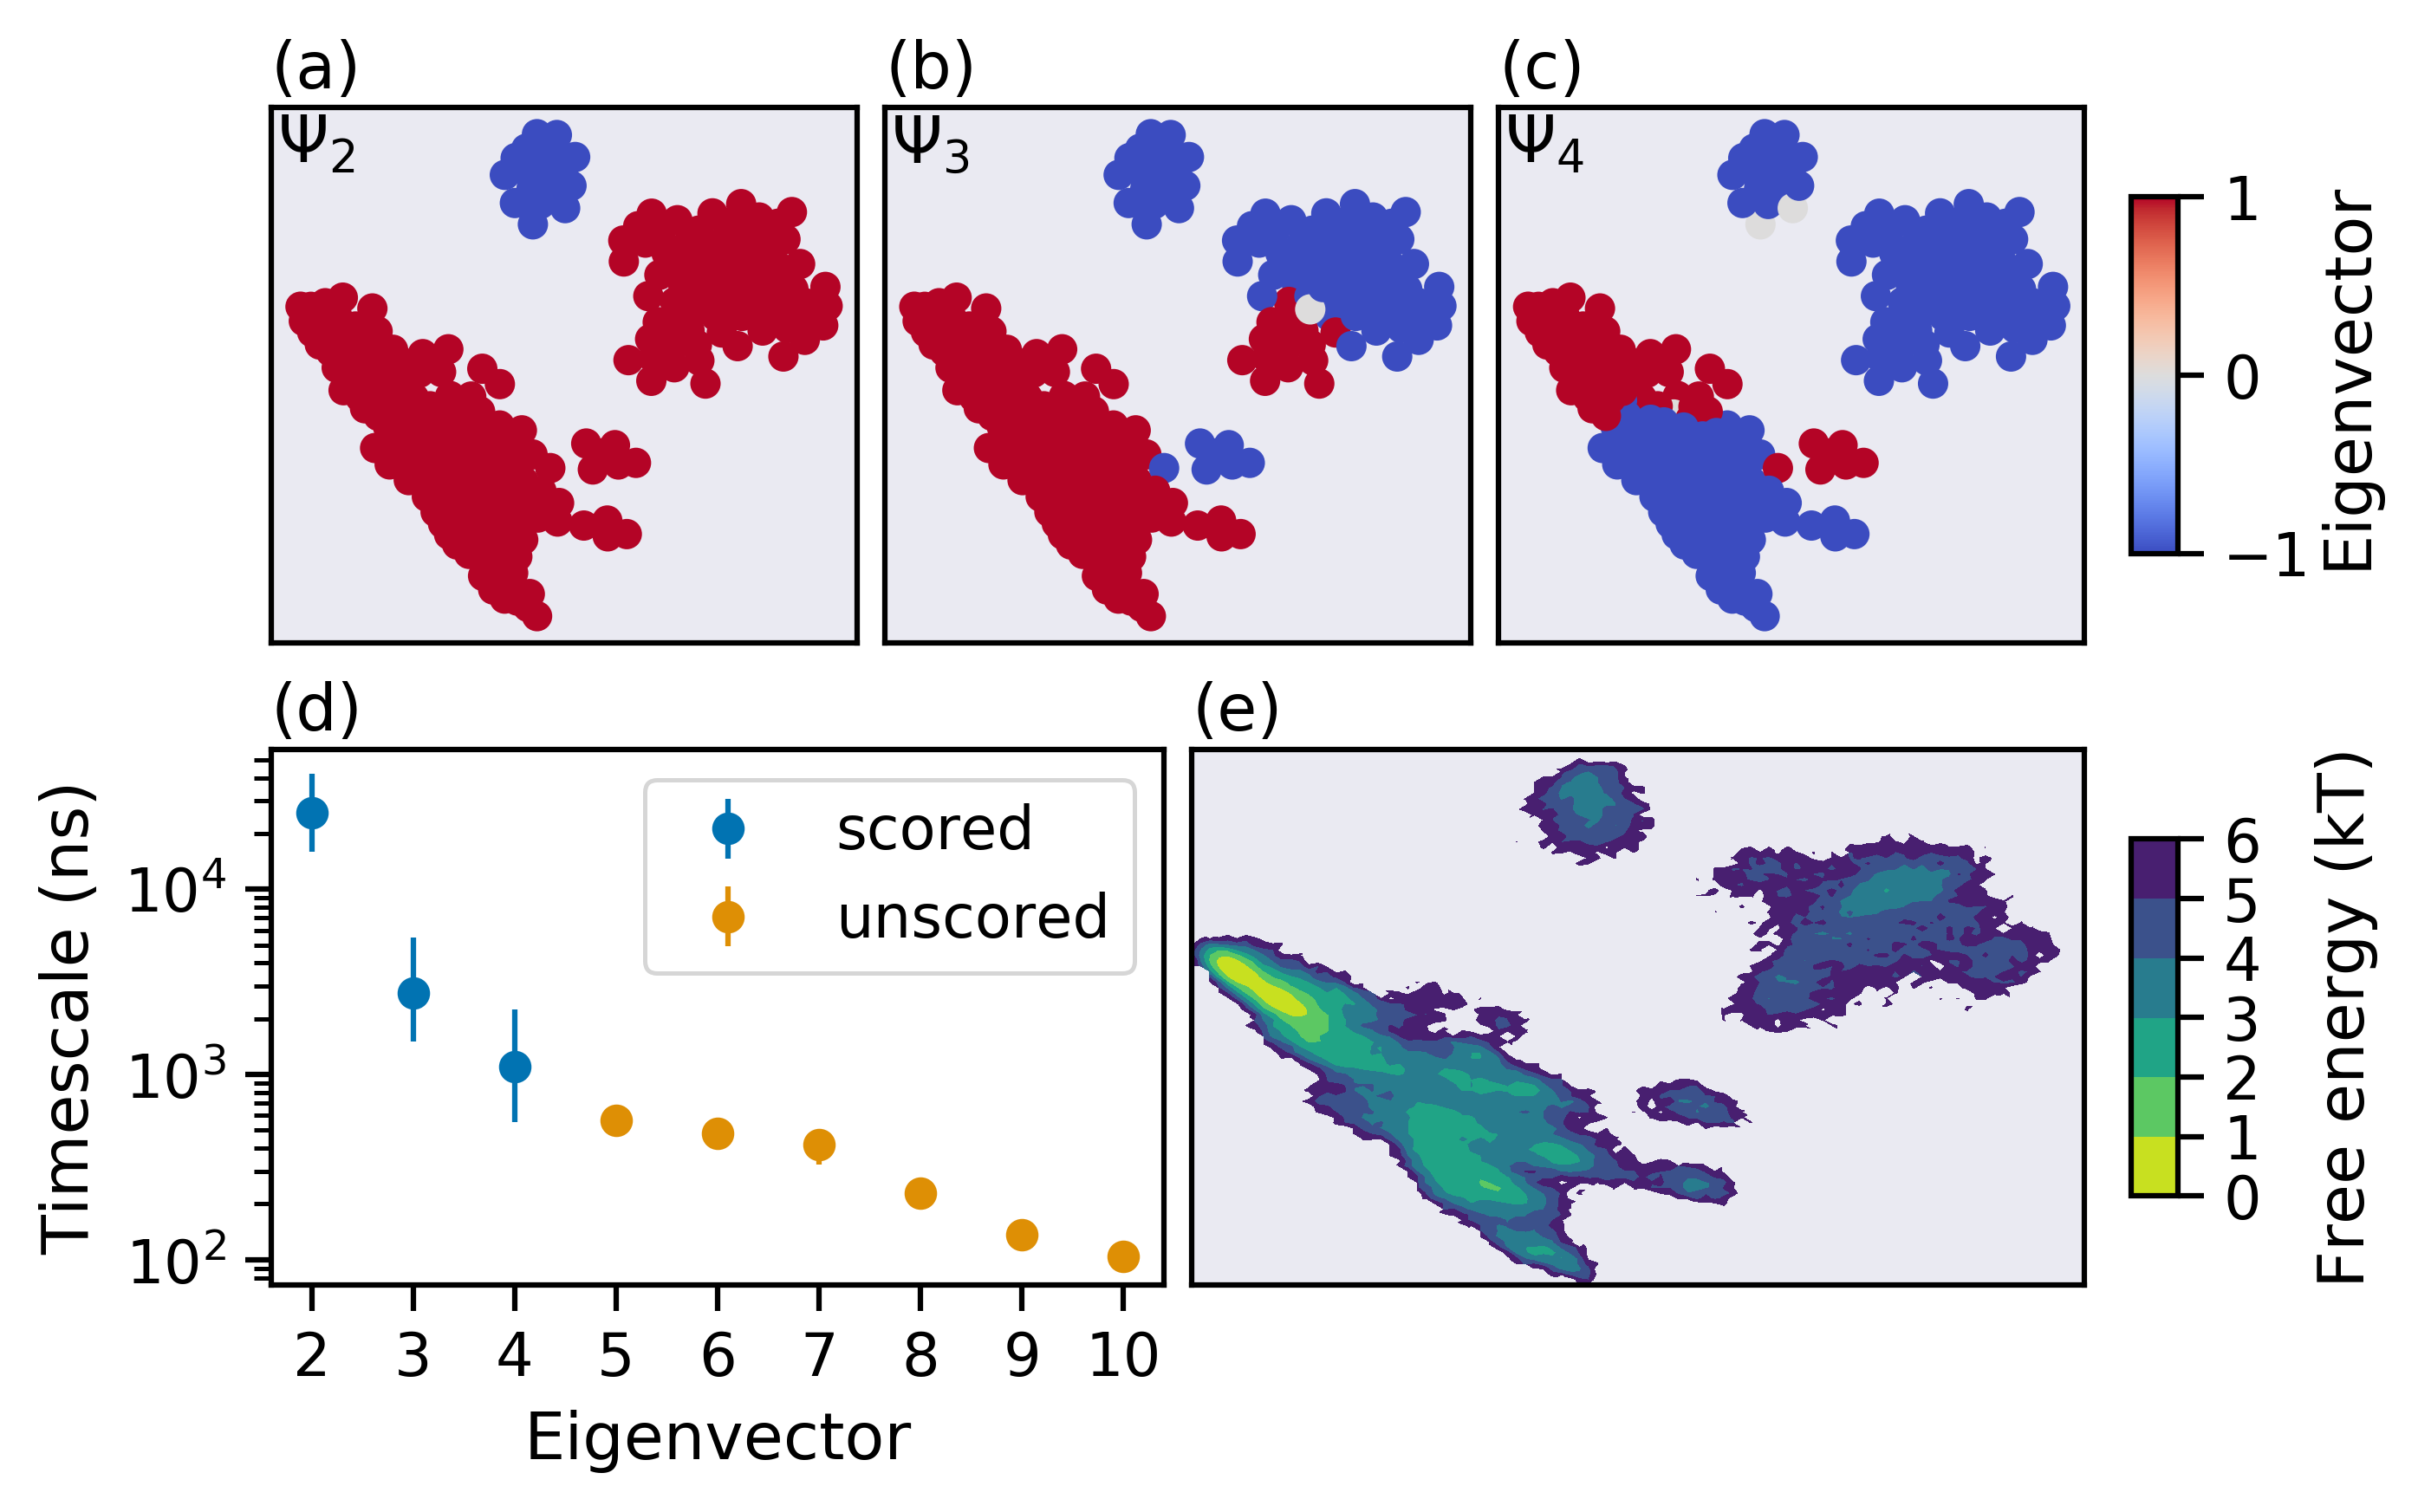
\includegraphics[width=0.7\textwidth]{chapters/msm_optimization/figures/aadh_msm_sens_1.png}
    \label{fig:aadh_msm_sens_1}
\end{figure}

Figure \ref{fig:aadh_msm_best} will serve as a base-case for a number of sensitivity analyses which are informed by the optimised response surface (figure \ref{fig:aadh_rsm_opt}) and eigenvalue spectrum (figure \ref{fig:aadh_its}).

Sensitivity 1 changed the MSM lag time from $\SI{2}{\nano\second}$ to $\SI{20}{\nano\second}$ and is shown in figure \ref{fig:aadh_msm_sens_1}. As expected the absolute values of the implied timescales have increased, as has the relative separation between $t_{2}$/$t_{3}$. The values of relaxation timescales are summarised in table \ref{tab:sens_ts}. The sign structure of the first and third relaxation process remains the same, but for the second and third relaxation process this has changed.  We can conclude that the first, definitely slow, relaxation process is robust with respect to it's sign structure. The second relaxation process which may or may not be dominant, changes its character as a function of the MSM lag time and so  $\tau(\mathrm{MSM}) = \SI{20}{\nano\second}$ will need to be included in the coarse graining analysis in chapter \ref{chap:hmm}. 

\begin{figure}
    \centering
    \caption{Sensitivity 2: MSM of AADH with the best hyper-parameters of with the interatomic distances feature ($\tau = \SI{1}{\nano\second}, m=2, n=110$) and $\tau(\mathrm{MSM}) \SI{2}{\nano\second}$. See caption of figure \ref{fig:aadh_msm_best} for details.}
    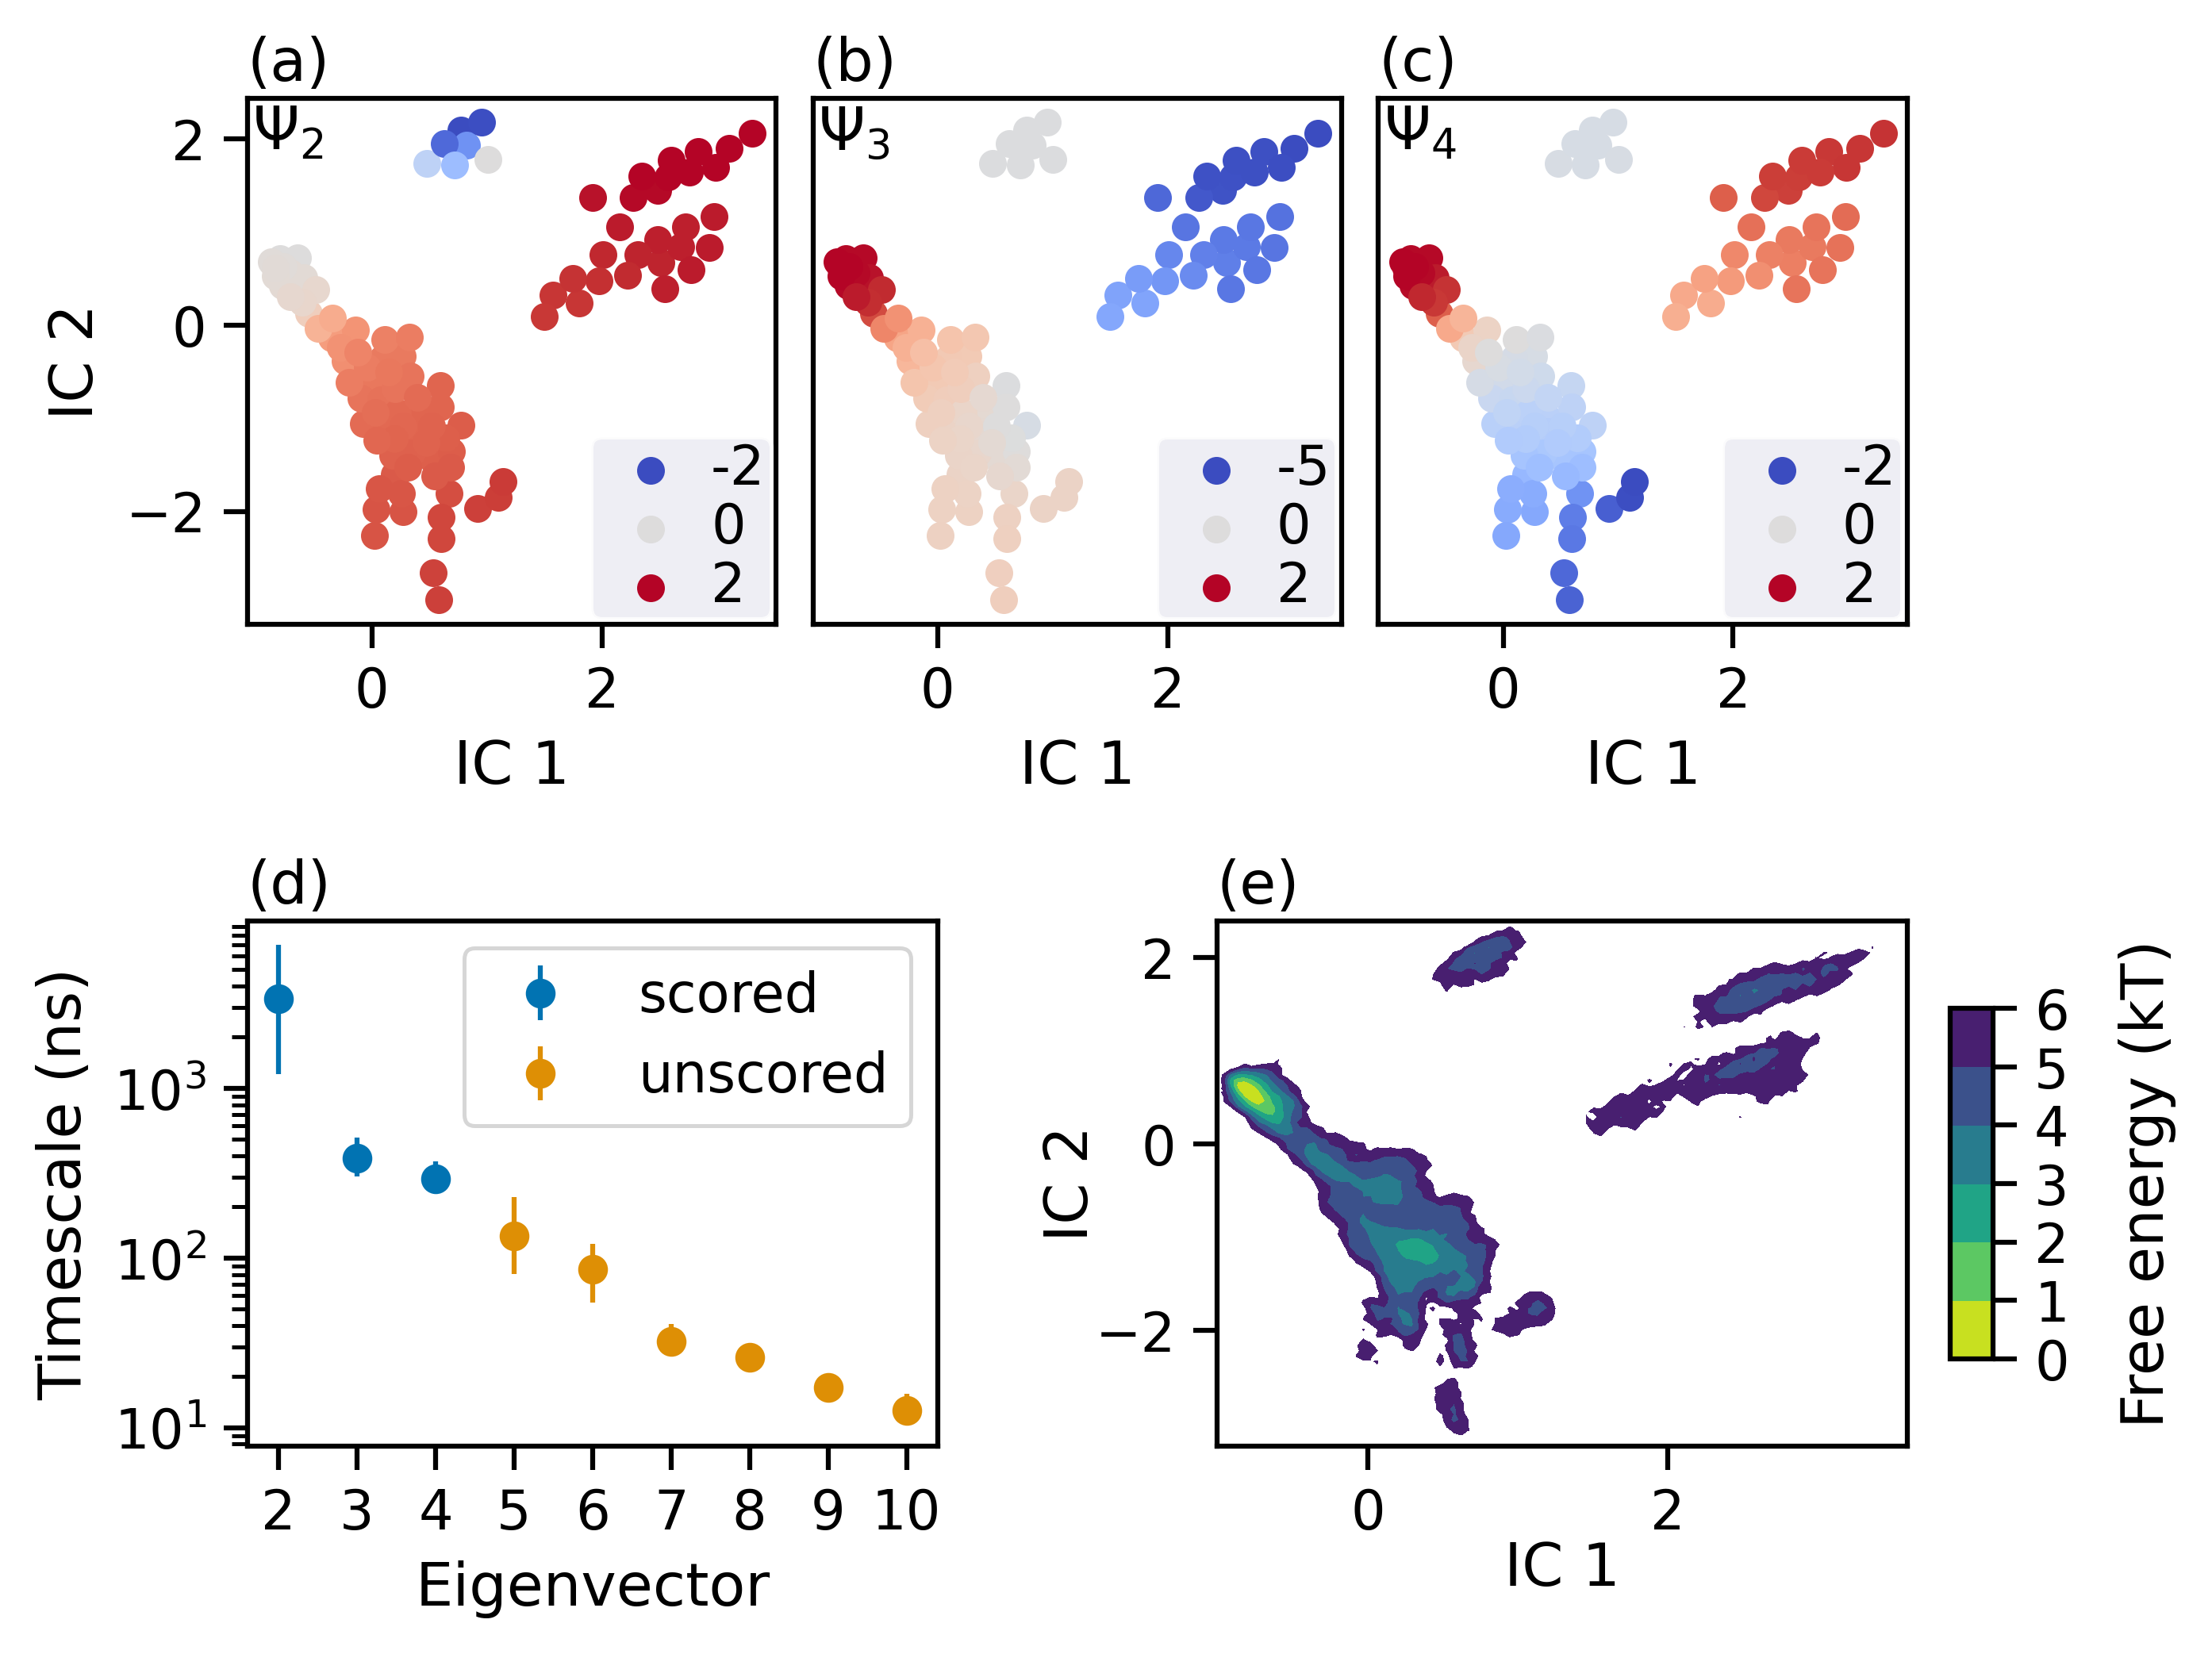
\includegraphics[width=0.8\textwidth]{chapters/msm_optimization/figures/aadh_msm_sens_2.png}
    \label{fig:aadh_msm_sens_2}
\end{figure}


Sensitivity 2 changed the hyper-parameters to the best performing set with the interatomic distances feature ($\tau = \SI{1}{\nano\second}, m=2, n=110$) and is shown in figure \ref{fig:aadh_msm_sens_2}.  This was justified because of the similarity in response values (incumbent: $\mu=3.56 \pm 0.18$, sensitivity 2: $\mu=3.44 \pm 0.35$). There is a clear similarity between sensitivity 2 and the base case in both the free energy surface and the first relaxation processes' timescale ($t_{2} = \SI{2.7}{\micro\second}$ cf.$t_{2} = \SI{2.2}{\micro\second}$ in the base case) and sign structure.  There is also a greater separation in timescales between $t_{2}$ and $t_{3}$ ($t_{2}/t_{3} \simeq 6$) than the base case ($t_{2}/t_{3} \simeq 2$). Taken together these two observations suggest that the interatomic distances resolve the first relaxation processes similarly but not the second relaxation process. 


\begin{figure}
    \centering
    \caption{Sensitivity 3: MSM of AADH with the same hyper-parameters of the MSM as the base case but a long TICA lag time $\tau = \SI{85}{\nano\second}$.  See caption of figure \ref{fig:aadh_msm_best} for details.}
    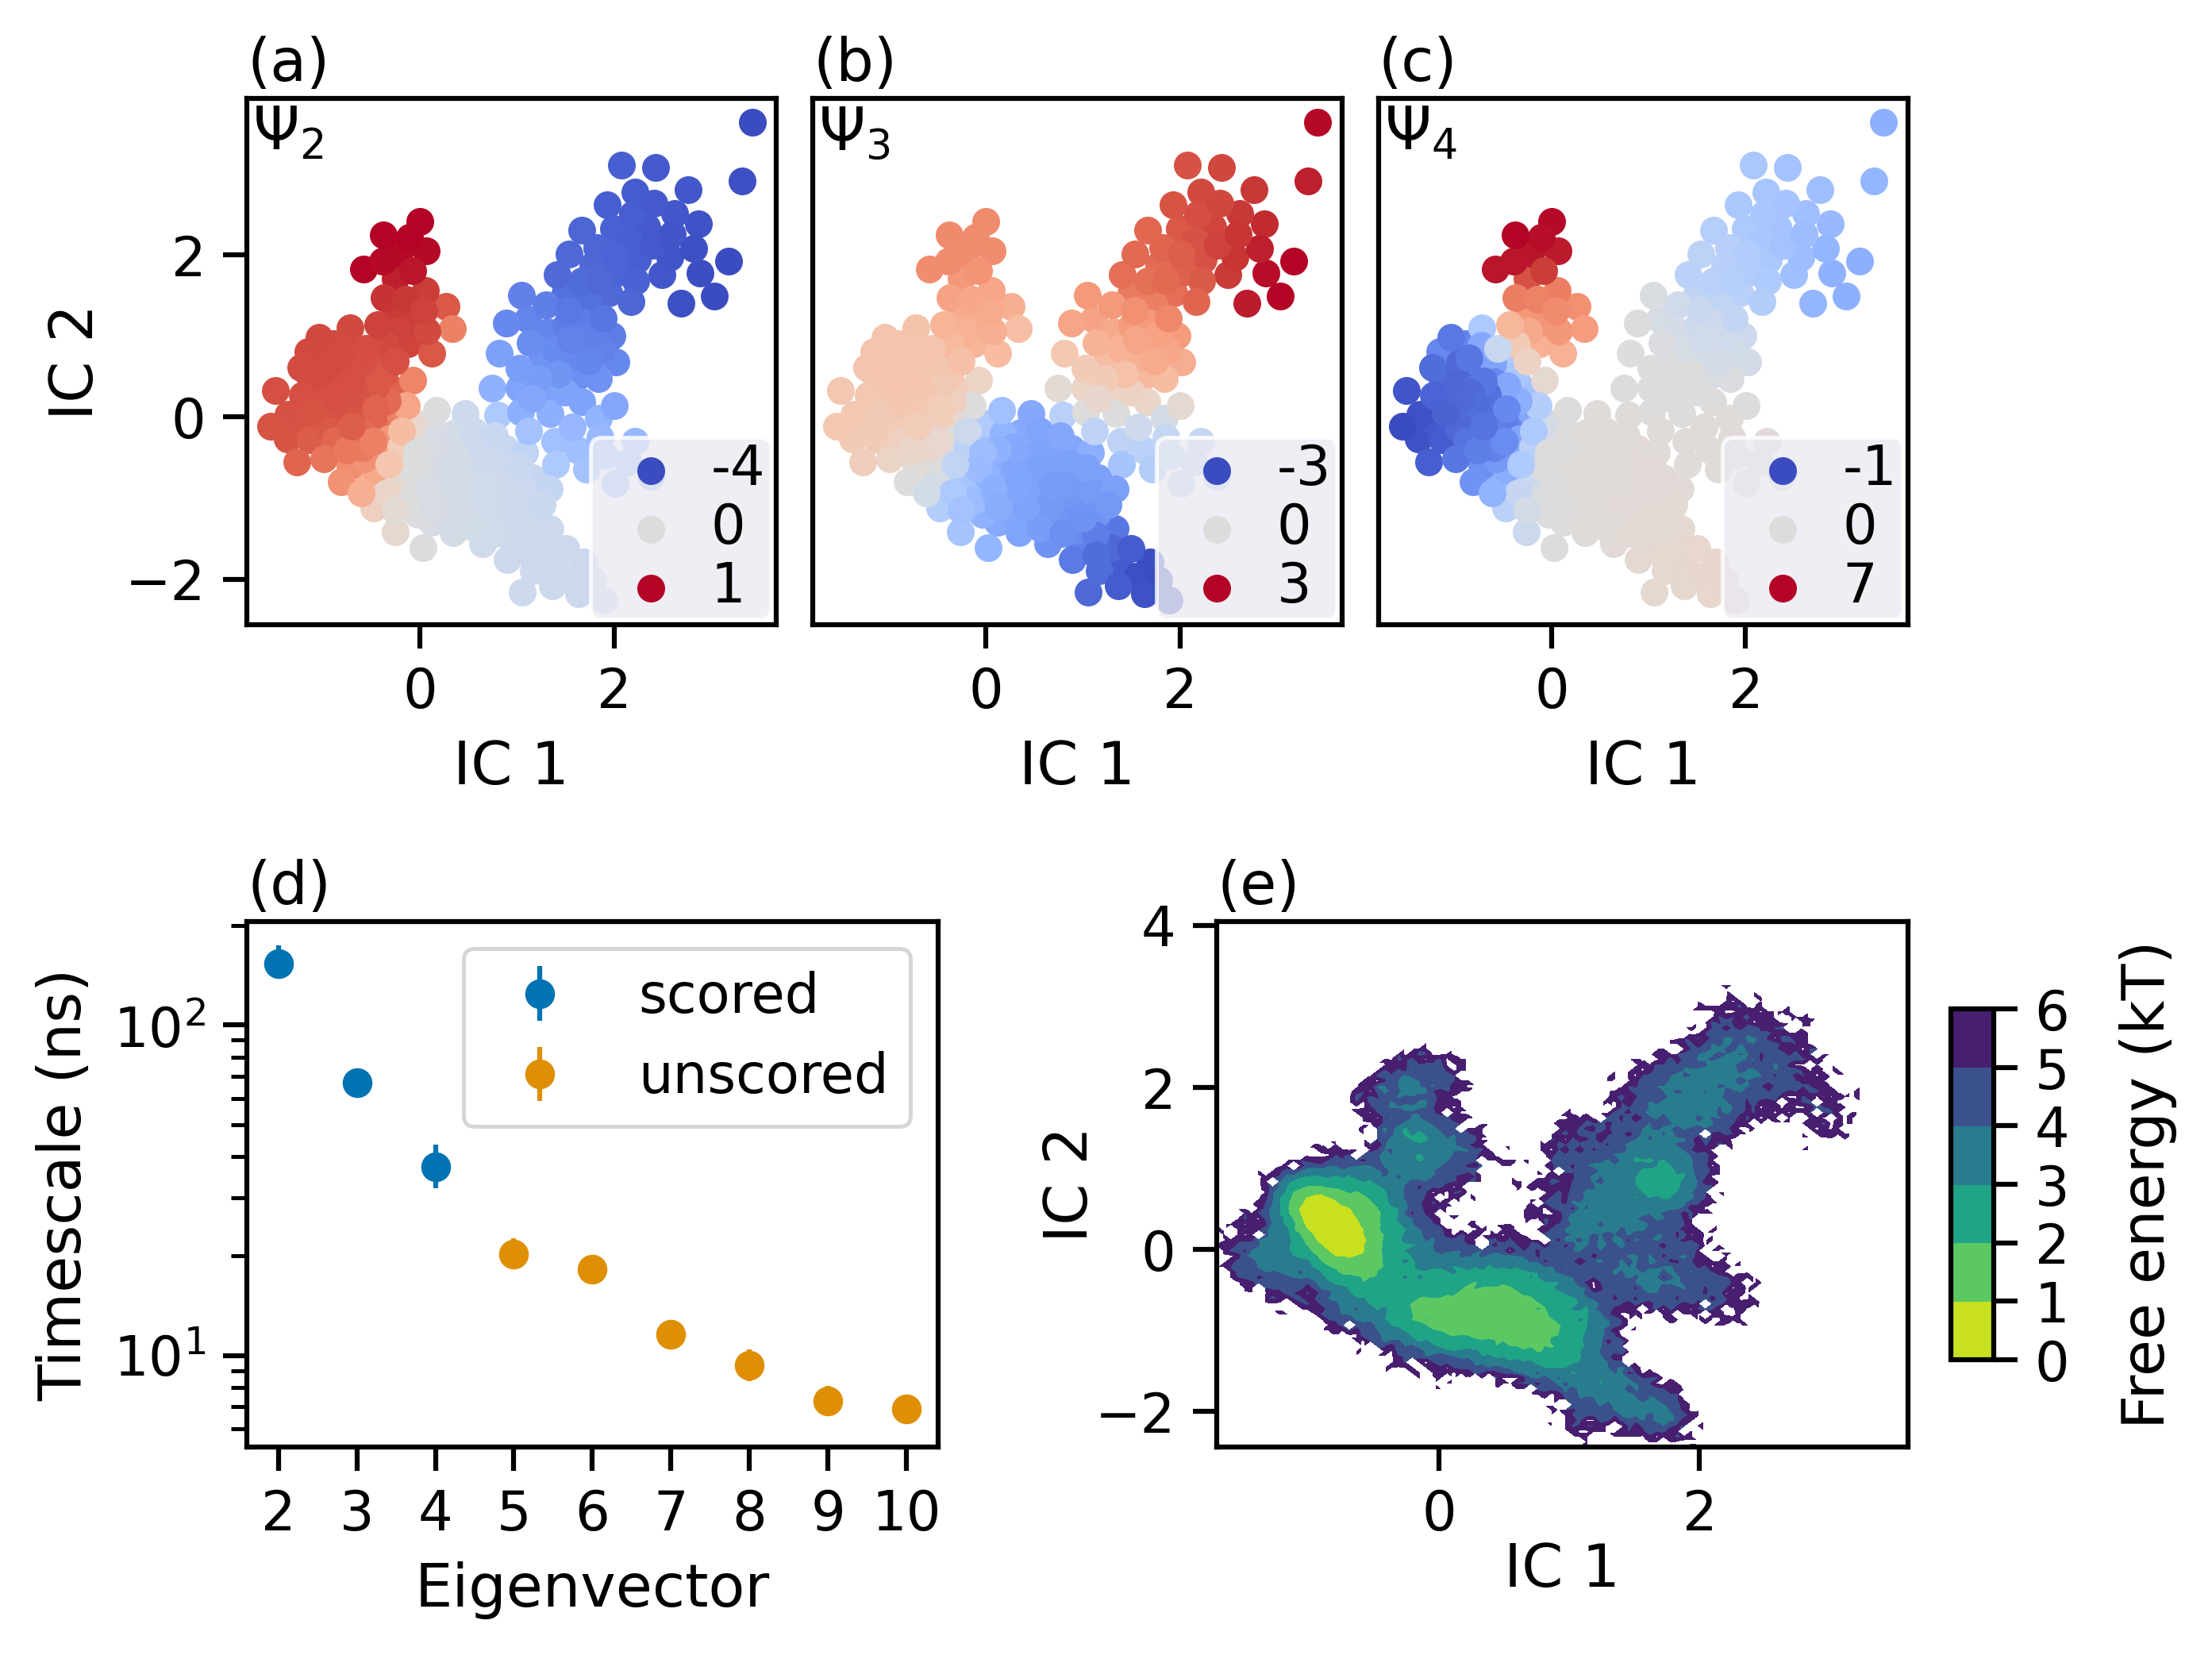
\includegraphics[width=0.8\textwidth]{chapters/msm_optimization/figures/aadh_msm_sens_3.png}
    \label{fig:aadh_msm_sens_3}
\end{figure}

\begin{figure}
    \centering
    \mycaption{Comparison of the first two TICA eigenvectors between base case, $\tau=\SI{10}{\nano\second}$ (blue) and sensitivity three $\tau=\SI{85}{\nano\second}$ (orange). The individual elements correspond to the weights associated with each of the $116$ dihedral features. Only the absolute values are shown. The elements were ordered according to the absolute value of the elements in the base case for each TICA component. The normalized overlap between the base case ($\mathbf{v}_{1}$) and sensitivity three ($\mathbf{v}_{2}$) is calculated as $\mathbf{v}_{1}\cdot\mathbf{v}_{2}/|\mathbf{v}_{1}||\mathbf{v}_{2}|$.}
    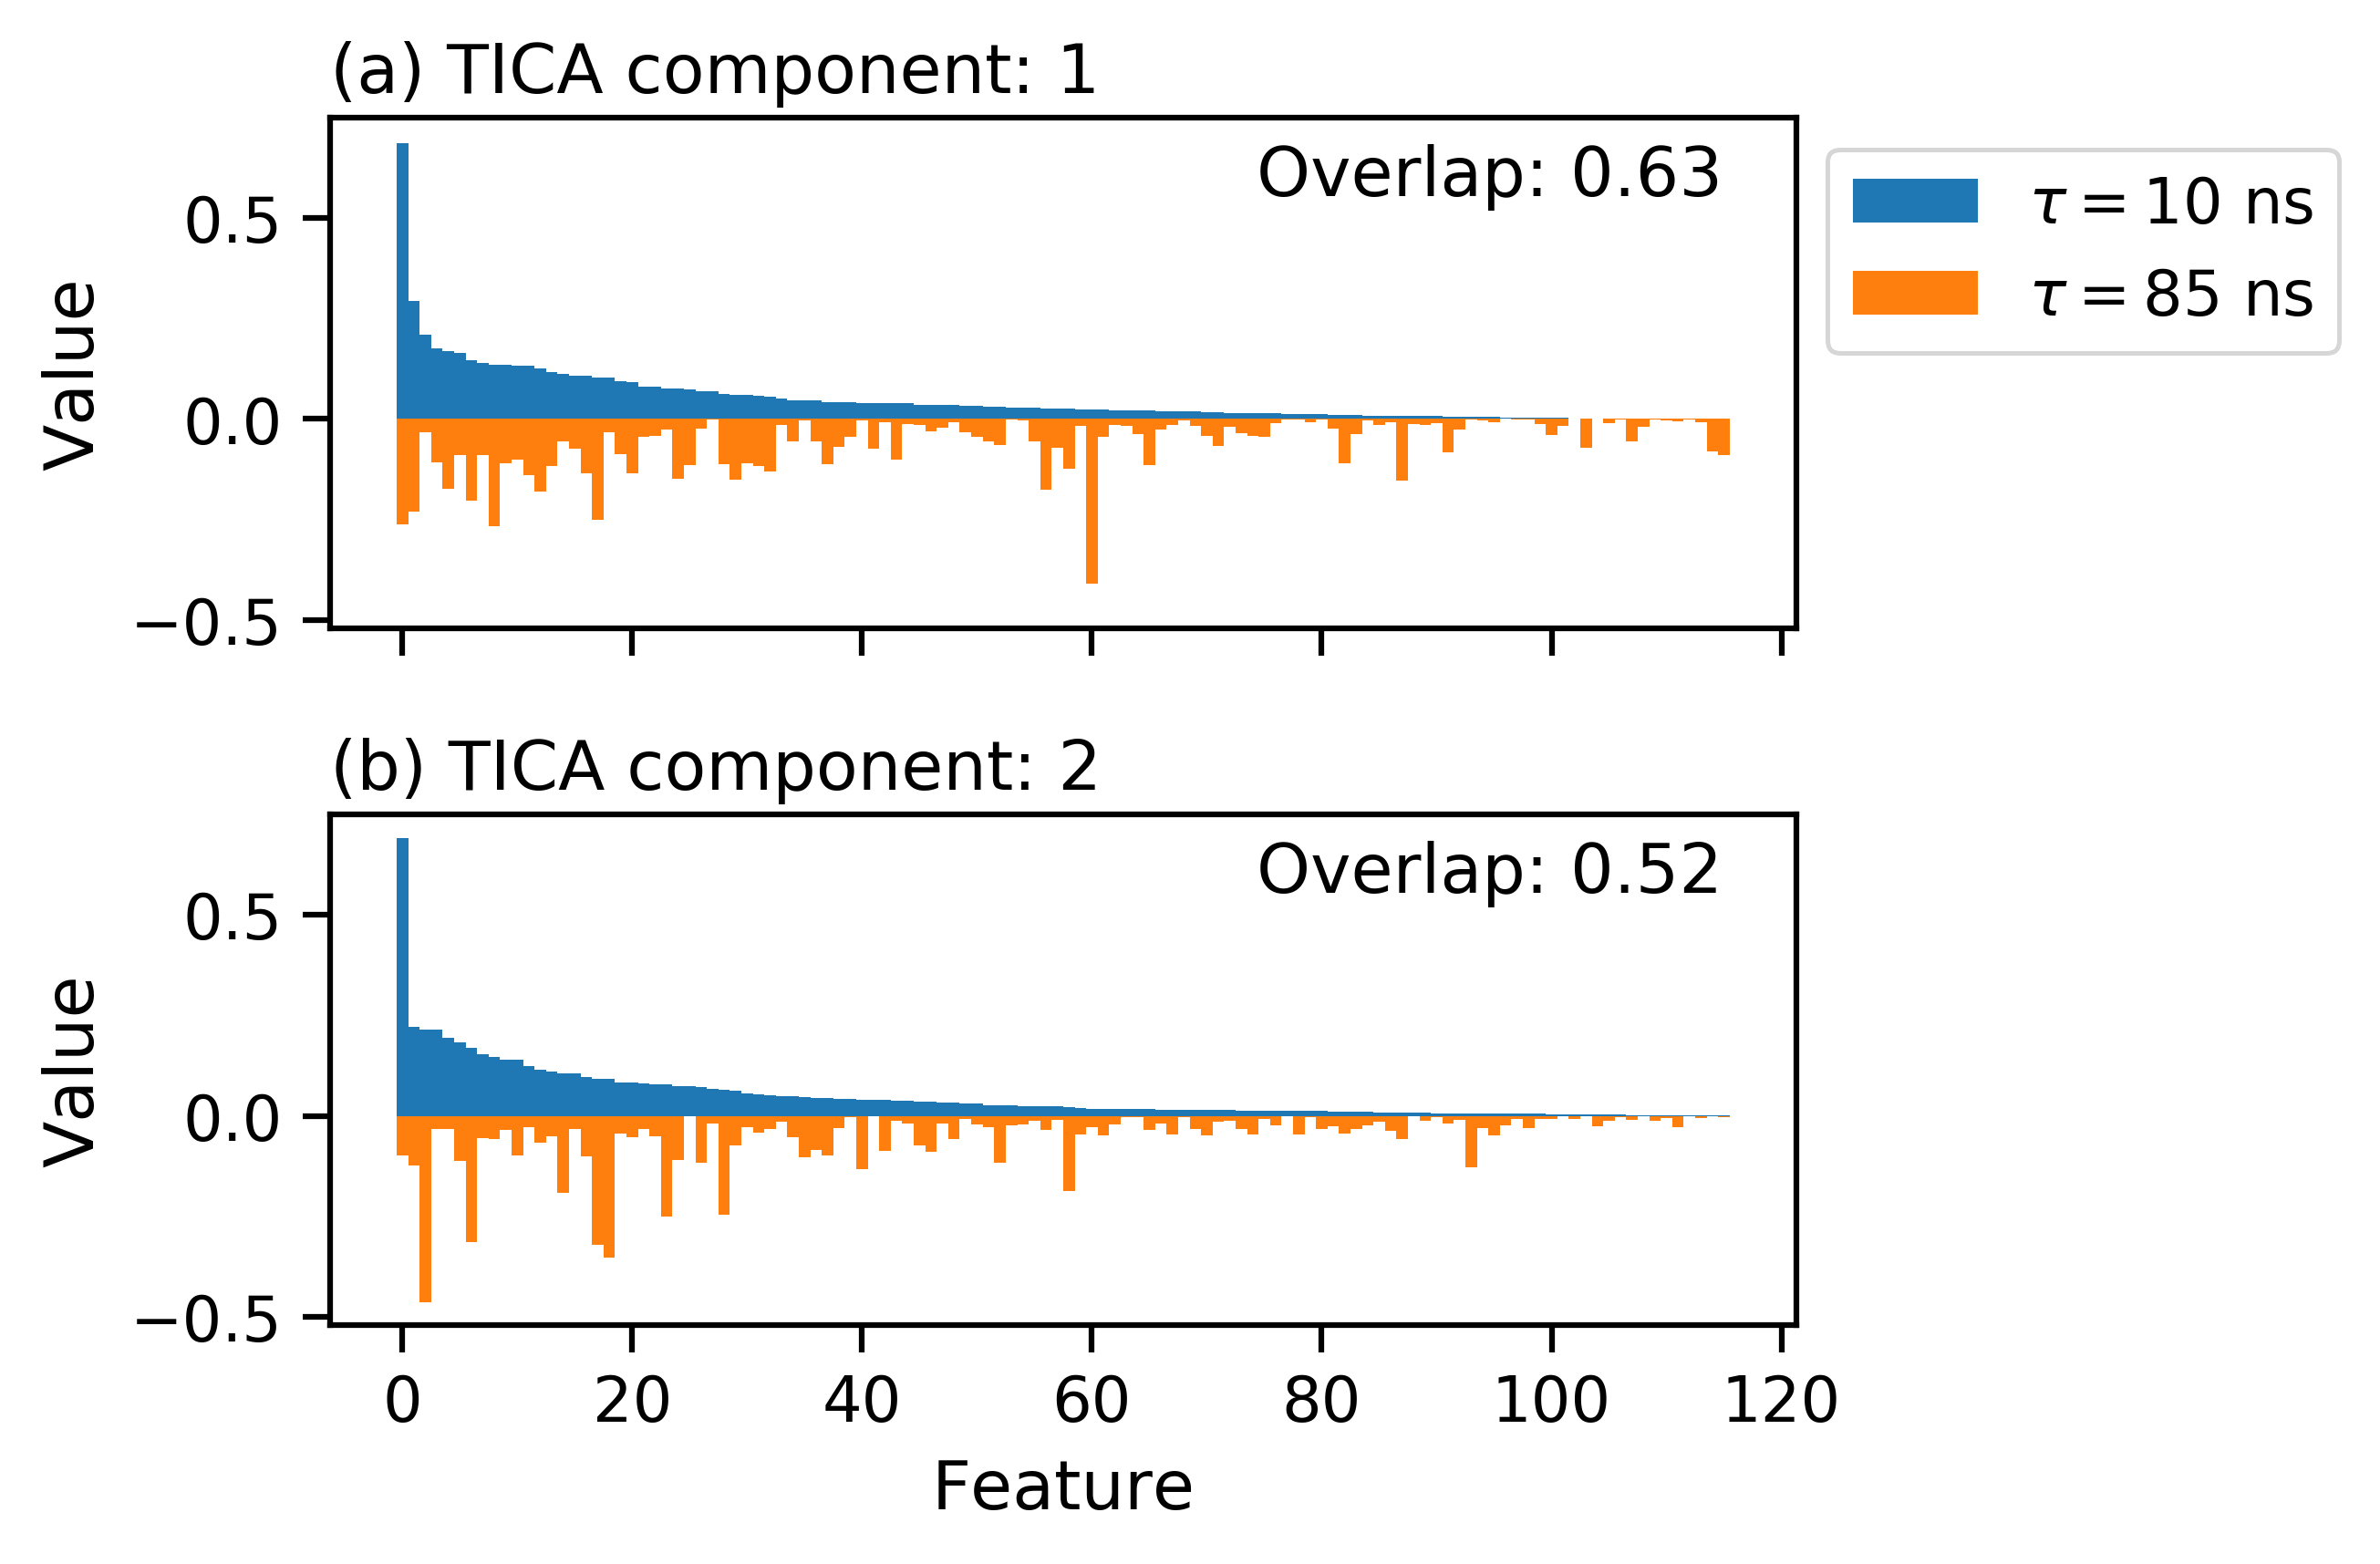
\includegraphics[width=0.8\textwidth]{chapters/msm_optimization/figures/aadh_msm_sens_3_tica.png}
    \label{fig:aadh_msm_sens_3_tica}
\end{figure}

Sensitivity 3, changed the value of $\tau$ to $\SI{85}{\nano\second}$ compared to the base case and is shown in figure \ref{fig:aadh_msm_sens_3}.   This value of $\tau$ was chosen because the response value at this point had the smallest  overlap with the incumbent (incumbent: $\mu=3.56 \pm 0.18$, sensitivity 3: $\mu=3.30 \pm 0.24$).  Here there is a distinct difference in the absolute values of the timescales and the free energy surface compared to the base case. To further delineate the difference between the two TICA representations, figure \ref{fig:aadh_msm_sens_3_tica} shows the difference between the first two TICA components. The  TICA components of the base case are shown in blue with the magnitude of the individual elements (corresponding to the $116$ dihedral features) ordered in decreasing value. The corresponding elements for this sensitivity are shown in orange with the sign flipped. The normalized overlap between the two TICA components of the base case and this sensitivity are $0.63$ and $0.56$  for the first and second TICA components respectively. This is due to the different weights attached to each dihedral feature. It is highly likely therefor that this represents a qualitatively and quantitatively different model. Where this change come in the response surface and and what the corresponding values of the response are will determine whether this an example of the Roshomon effect. 

\begin{table}
    \centering
    \mycaption{Mean implied timescales and $\SI{95}{\percent}$ credible intervals (in nanoseconds) of the relaxation processes 2 - 10 for the base case and three sensitivities.}

    \begin{tabular}{|l|l|l|l|l|}
    \hline
     &             Base Case &            Sensitivity 1 &         Sensitivity 2 &      Sensitivity 3 \\
    Process &                       &                          &                       &                    \\
    \hline\hline
    2       &  2,117 (1,033, 5,214) &  25,843 (15,913, 41,797) &  2,694 (1,352, 4,606) &   152 ( 138,  169) \\
    3       &     988 ( 479, 1,669) &     2,748 (1,510, 5,458) &      408 ( 312,  716) &    67 (  64,   71) \\
    4       &      231 ( 195,  276) &      1,101 ( 553, 2,256) &      304 ( 234,  397) &    36 (  31,   43) \\
    5       &      138 ( 129,  149) &         563 ( 497,  668) &      155 (  79,  252) &    20 (  19,   23) \\
    6       &       54 (  43,   73) &         482 ( 412,  566) &       80 (  52,  115) &    18 (  17,   20) \\
    7       &       38 (  33,   43) &         418 ( 327,  463) &       30 (  26,   38) &    12 (  11,   13) \\
    8       &       23 (  21,   26) &         228 ( 205,  249) &       25 (  22,   29) &     9 (   8,   10) \\
    9       &       21 (  18,   23) &         137 ( 115,  163) &       17 (  15,   18) &     7 (   7,    8) \\
    10      &       16 (  15,   19) &         105 (  99,  110) &       12 (  11,   15) &     7 (   6,    7) \\
    \hline
    \end{tabular}
    \label{tab:sens_ts}
\end{table}


\section{Conclusions}\label{sec:msm_opt_conc}

This chapter introduced the use of response surfaces and Bayesian optimisation for understanding and optimizing the hyper-parameters of an MSMs. A GP model proved a satisfactory statistical model for estimating the response surface of alanine dipeptide with two predictors $\chi$ and $n$. Model selection, using standard GP metrics, selected the logarithmic input warping over the hyper-parameter $n$ to make the stationary assumption of the GP more plausible.  While GPs are usually used with continuous predictors the use of dummy coding  was demonstrated to be effective in incorporating the protein feature, $\chi$, as a categorical predictor. The relevance, a GP kernel hyper-parameter corresponding to each predictor,  was shown to reflect the importance of each  MSM hyper-parameter. For the non-categorical hyper-parameter, $n$, the low relevance was a reflection of the near flat response of the MSM to changes in $n$. For the categorical predictor, the protein feature $\chi$, the low relevances of each feature was a reflection of how similar the response surfaces were \emph{conditional} on the value of $\chi$, in other words, how much information sharing there was between the different features. 

The response surface for AADH, with four predictors ($\chi$, $\tau$, $m$ and $n$) was also fit with a GP. The conditional structure of the predictor space meant that the RMSD feature was not able to be incorporated into the response surface. This is a problem for GPs in this setting. In future work more flexible models, such as Random Forests or Tree Pazen Estimators could be used to model this conditional structure more effectively. Model selection was used to select the most appropriate GP kernel and input warping. The final selected model fit the model with varying success. Overall the model fit the data well, but for the best performing feature, $(\phi, \psi, \chi)$ dihedrals, the fit was less satisfactory. 

The relevance of the hyper-parameters revealed once again that $n$ was not important in determining the response, while the TICA hyper-parameters were the most relevant. While the $(\phi, \psi, \chi)$ dihedrals and interatomic distances features were the best performing, each of the features did not have high relevance. This indicated that the response surfaces conditional on the features were similar.  The relative relevance of the hyper-parameters was shown to be useful in visualising the high dimensional surface.

Bayesian optimisation was used to in an attempt to optimise the AADH response surface. After fitting the response surface with $361$ randomly sampled hyper-parameters, further Bayesian optimisation did not increase the value of the maximum of the response surface or change significantly the optimal hyper-parameters. Bayesian optimisation was also used on subsets of the data and the resulting optimum hyper-parameters, determined from a total of $150$ trials, were similar to those determined from the full hyper-parameter trial data set. This suggests the Bayesian optimisation could be used seeded with $25$ random observations per MSM hyper-parameter. Further work is needed to determine the most efficient combination of random sampling and Bayesian optimisation. 

Once the response surface was optimised and the best performing MSM hyper-parameters determined,  inspection of resulting MSM eigenvalue spectrum and the response surface suggested a number of sensitivity tests to be performed.  These tests revealed a fairly robust single dominant relaxation process with associated time-scale of $\SI{2.12}{\micro\second} (\SIrange{1.0}{5.2}{\micro\second})$. A second dominant relaxation process was not ruled out. The most relevant parameters, the TICA lag time, was also associated with changing both the qualitative and quantitative nature of the MSM. This could be an example of the Rashomon effect, something described in the MSM literature. 


% The response of an MSM to a randomly selected set of hyper-paraImeters was measured using standard the MSM metric, VAMP-2. These data were used with Gaussian process regression (GPR) to model the response surface of the MSM. Input warping and the type of kernel used in the  GPR were chosen using cross-validation of the standardised log loss and squared error metrics.  Bayesian optimisation was used to find the optimum of the response surface using the expected improvement as a hyper-parameter selection policy. Once the optimum had been found and the corresponding MSM was estimated, the response surface and eigenvalue spectrum was used to explore the robustness of the optimum hyper-parameters with a series of sensitivity tests. 






\section{Appendix}\label{app:msm_opt}

